A detailed description of the SNO+ detector has been implemented in the \texttt{RAT} software package for Monte Carlo (MC) simulations, as mentioned in Chapter 3. However, when the simulations are compared to the real world, there always exist discrepancies. To make precise measurements, calibration sources were implemented in the SNO+ detector during the water phase and the partial-fill phase. During the water phase, the $^{16}$N source (described in Sect.~\ref{sect:n16}) was used for the primary detector calibration. The $^{16}$N calibration data ($^{16}$N runs) were mainly used to check the performance of the reconstruction algorithms for event position, direction, and energy. 

In this chapter, the \texttt{MPW fitter} (described in Sect.~\ref{sect:mpw}) was applied on both the experimental data from, and simulations of, the $^{16}$N runs in the water phase. By analyzing the differences between the $^{16}$N data and corresponding MC simulations, systematics of the position and direction reconstruction were extracted, and these were used in the solar neutrino analysis of Chapter 6. The event energy was reconstructed by the SNO+ energy fitter for the water phase (described in Sect.~\ref{sect:energyFitter}), which utilizes the \texttt{MPW fitter}'s event vertex and direction. Also, based on the \texttt{MPW fitter}'s reconstructed vertex and direction other parameters, such as the in-time-ratio (ITR) and the isotropy parameter ($\beta_{14}$) were calculated.

\section{$^{16}${N} Calibration Scans in the Water Phase}\label{sect:n16_water}

During the water phase, in June and in November 2017 the $^{16}$N source was deployed at different positions inside the AV to perform internal calibration scans, and in March 2018 it was deployed at various positions in the external water region between the AV and the PSUP to perform external scans. For each $^{16}$N run, the source was placed at a fixed position, and data were collected for about 20 minutes (with the exception of run 107055 with the source at PSUP centre, for which run time was 1 hour). For some of the internal scans the source was moved along $(x,y,z)$-axes (these scans being named ``X, Y, Z scans'' in this thesis), and in others it was moved diagonally across the AV and placed at the corners of the inner AV (``corner scans''). For the external scans, the source was placed in the external water region outside the AV. The source was moved along the $z$-axis with a fixed $(x,y)$ position close to the AV, at (-5861.0,-2524.0)~mm. Fig.~\ref{N16_3Dscan} shows the different positions of the source deployment. In this thesis, 79 internal scan runs were used. Details of the calibration runs are listed in the tables in Appendix.~\ref{appendix:calibration}. %%%%%% and 19 external runs

\begin{figure}[!htb]
	\centering
	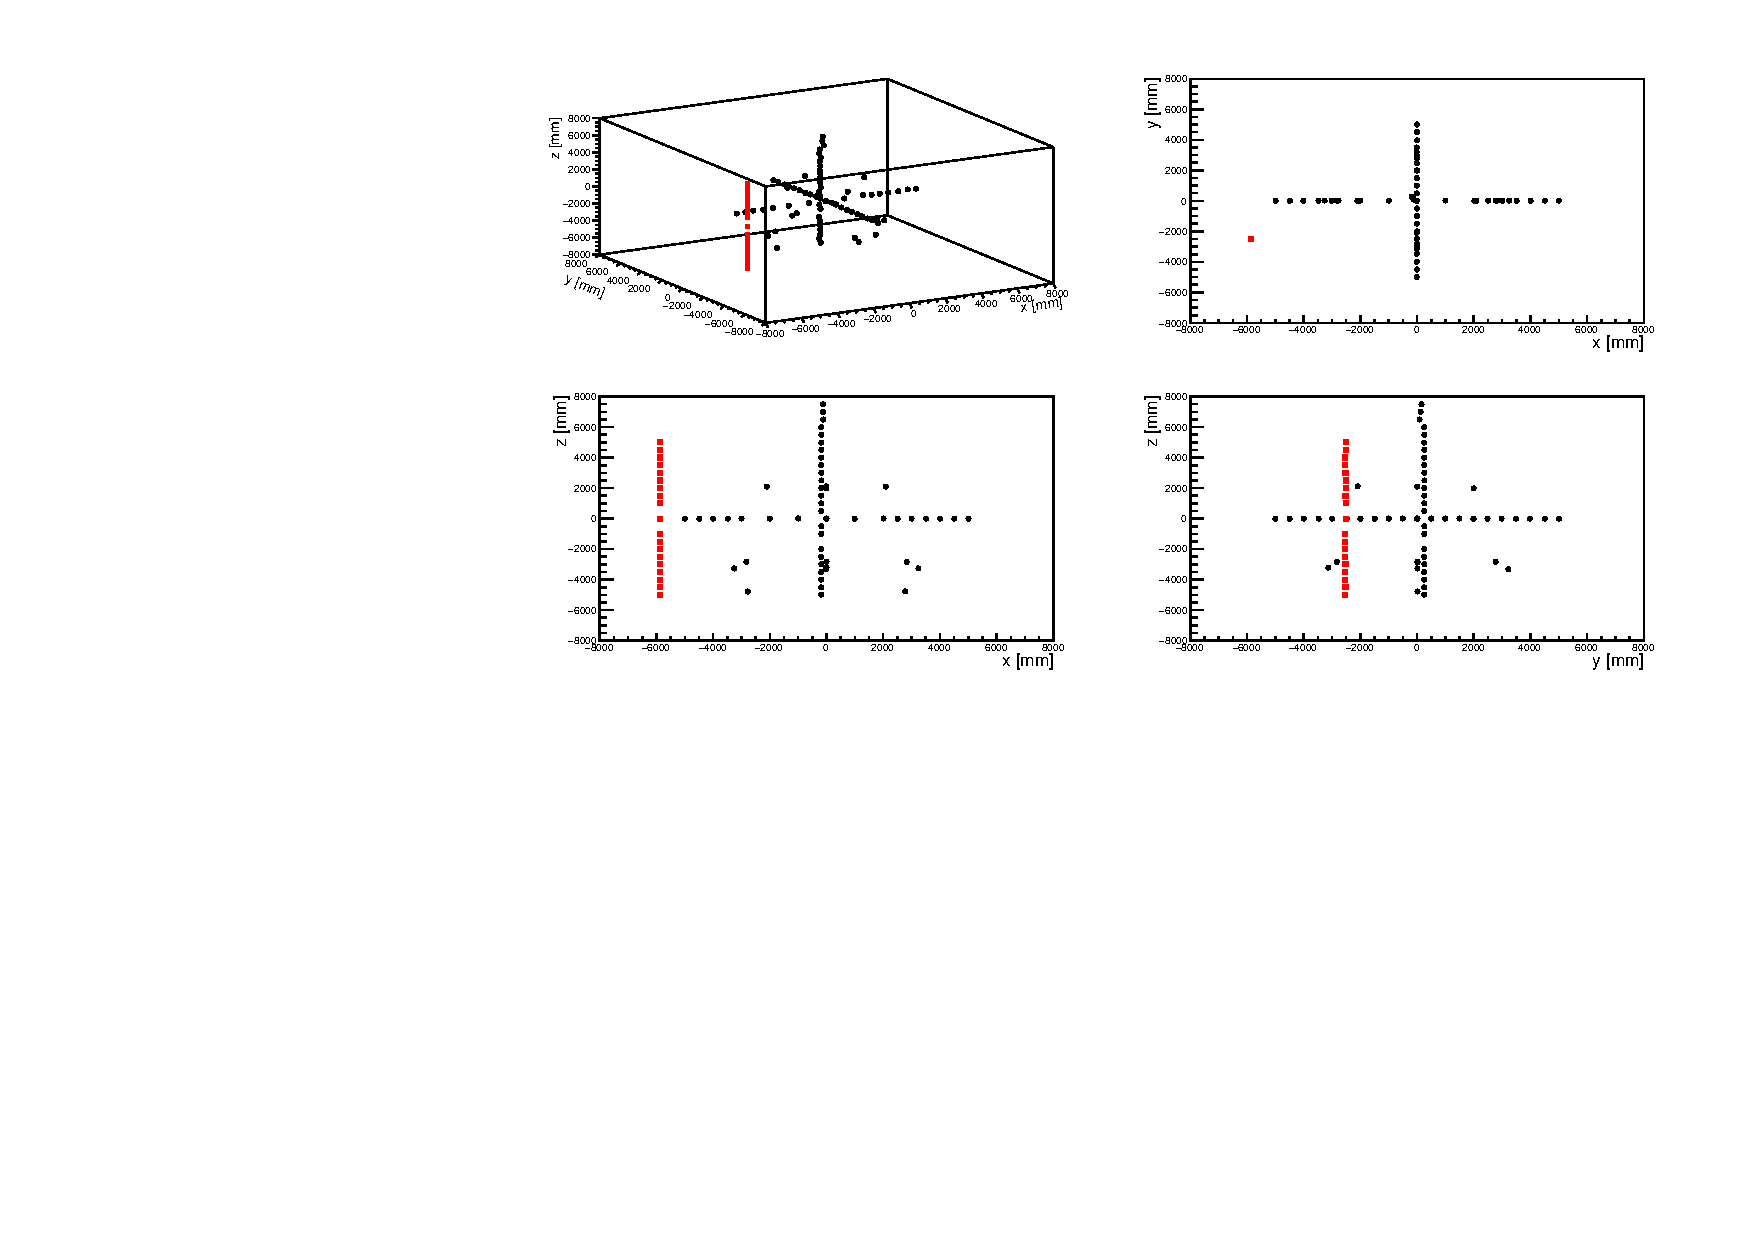
\includegraphics[width=15cm]{N16_3Dscan.pdf}
	\caption[The deployed source positions of the $^{16}$N scan runs.]{The deployed source positions of the $^{16}$N scan runs used by this thesis. The black dots are internal runs while the red squares are external runs.	\label{N16_3Dscan}}
\end{figure}

The $^{16}$N calibration runs provide an ideal test of fitter performance. From a comparison of reconstructions for data and MC, we can extract the resolution and bias of the fitter. Here I determined the performance of both the \texttt{RAT water fitter} and the \texttt{MPW fitter} for vertex and direction reconstruction, characterizing that performance in terms of statistics pertaining to vertex shift (or offset), and uncertainty. 

When analyzing $^{16}$N run data and simulations, an FECD tag cut (FECD$==9188$) was applied during data processing, to save the events only when the source trigger fired. A reconstruction threshold ($\mathrm{NHits}>5$) was applied to the MC and data. In addition to these cuts, high-level cuts based on classifiers were used. 

\section{High Level Cuts for the Water Phase}\label{sect:high_level_cuts}

A set of (event-) classifiers, developed originally for the SNO analysis, have been adjusted and optimized for the SNO+ water phase analysis\cite{highlevel}. These event classifiers utilize reconstructed quantities, so they always require a valid reconstruction.

\begin{itemize}
	\item[$\bullet$] In time ratio (ITR) classifier
	
	For each event, this classifier loops through the triggered PMTs (hits), calculates $t_{res}$ for each, and determines the fraction of hit PMTs for which $t_{res}$ falls within an optimized `prompt time window'. In the water phase, the time window was $[-2.5,5.0]$~ns. If the ITR ratio is too low for an event, a large proportion of the hit PMTs were not triggered prompt light, suggesting that the event probably did not originate from Cherenkov light; it could be instrumental noise, or caused by a large amount of light reflecting off detector components (called ``late light''). 
	
	\item[$\bullet$] $\theta_{ij}$ isotropy classifier

	This classifier describes the angle subtended at an event vertex by PMT \#i and PMT \#j, as defined by:
	\begin{equation}
	\cos\theta_{ij}=\frac{(\vec{X}_{PMT\#i}- \vec{X}_\mathrm{event})\cdot (\vec{X}_{PMT\#j}- \vec{X}_\mathrm{event})}{|\vec{X}_{PMT\#i}- \vec{X}_\mathrm{event}||\vec{X}_{PMT\#j}- \vec{X}_\mathrm{event}|}\;.
	\end{equation}
	%% John: Jie, is this number, or rather, set of numbers, really an event classifier? There are, what, $N^2$ values of this property for EACH event? So it is not a single number for a given event. I wonder whether actually it is just needed as an input for $\beta_{14}$? Maybe I'm wrong, but it seems out of place, it doesn't have the same character as ITR and beta14 John
	\item[$\bullet$] $\beta_{14}$ isotropy classifier
	
	This classifier is derived from the event's {\em set} of angles $\theta_{ij}$. The first ($\beta_1$) and the fourth ($\beta_4$) spherical harmonics of an event are determined from
	\begin{equation}
	\beta_l = \frac{2}{N(N-1)}\sum_{i=1}^{N-1}\sum_{j=i+1}^N P_l(\cos\theta_{ij}) \; ,
	\end{equation}
	where $N$ is the selected NHit used by the reconstruction (see Sect.~\ref{sect:positionFoM}), and the $P_l(\cos\theta_{ij})$ are Legendre polynomials, and (following the precedent of the SNO collaboration) the linear combination $\beta_{14}=\beta_1+4\beta_4$ is taken. For a set of events produced by Cherenkov light, the corresponding set of values of $\beta_{14}$ has a Gaussian-like distribution \cite{dunmore2004separation}. In principle, any systematic deviation of $\beta_{14}$ from zero suggests some polarity or a deviation from a totally isotropic pattern.
	
\end{itemize}

\subsection{Effects of the High-level Cuts}

As described above, the classifiers can help to distinguish the physical events from Cherenkov events and nonphysical events from non-Cherenkov events, such as instrumental noises. To remove the non-Cherenkov background events such as instrumental noises, cuts of $\mathrm{ITR}>0.55$ and $-0.12<\beta_{14}<0.95$ (termed ``high-level cuts'') were suggested by the collaboration\cite{waterunidoc}. These cuts are based on the analysis of simulated physics events, as well as the experience gathered by the SNO collaboration \cite{waterunidoc,marzec2019measurement,dunmore2004separation}. %John: {red}(Jie it was not clear to me what you meant by ``analyses of data cleaning'' so I took it out. If the idea you were expressing is important, it needs to be expressed more clearly.){red}

The $^{16}$N central run 107055 data and (corresponding) MC simulation were used to check the effects of the high-level cuts. For the MC (data), the cut ITR$>0.55$ removed 0.69\% (0.79\%) of the total events and the cut $-0.12<\beta_{14}<0.95$ removed 1.11\% (0.93\%) of the total events. Combining the ITR and $\beta_{14}$ cuts, 1.69\% (1.62\%) of the total events were removed.

Poorly reconstructed events with large position bias ($>6000~$mm) were counted. For the MC case, the position biases were taken as the distance between the reconstructed position and the true (MC) position, $|\vec{X}_{fit}-\vec{X}_{MC}|$. For the data however, the bias was taken as the difference between the reconstructed position and the source manipulator position, $|\vec{X}_{fit}-\vec{X}_{src}|$\footnote{The source manipulator position is mainly measured by the ropes in the source manipulator system described in Sect.~\ref{sect:calibr}.}. Events with (so-defined) bias exceeding 6000 mm made up 0.13\% of the total event count, both in the MC and experimental calibration data. The high-level cuts removed 73.12\% (66.82\%) of these from the population of MC (data) events. In summary, the high-level cuts remove more than half of the events having large (reconstructed) position offset, while removing only about 1.6\% of the total events. 

Fig.~\ref{n16_highLevelCut} shows the relations between the position biases and the ITR, $\beta_{14}$ respectively, for the data and MC.
\begin{figure}
	\centering
	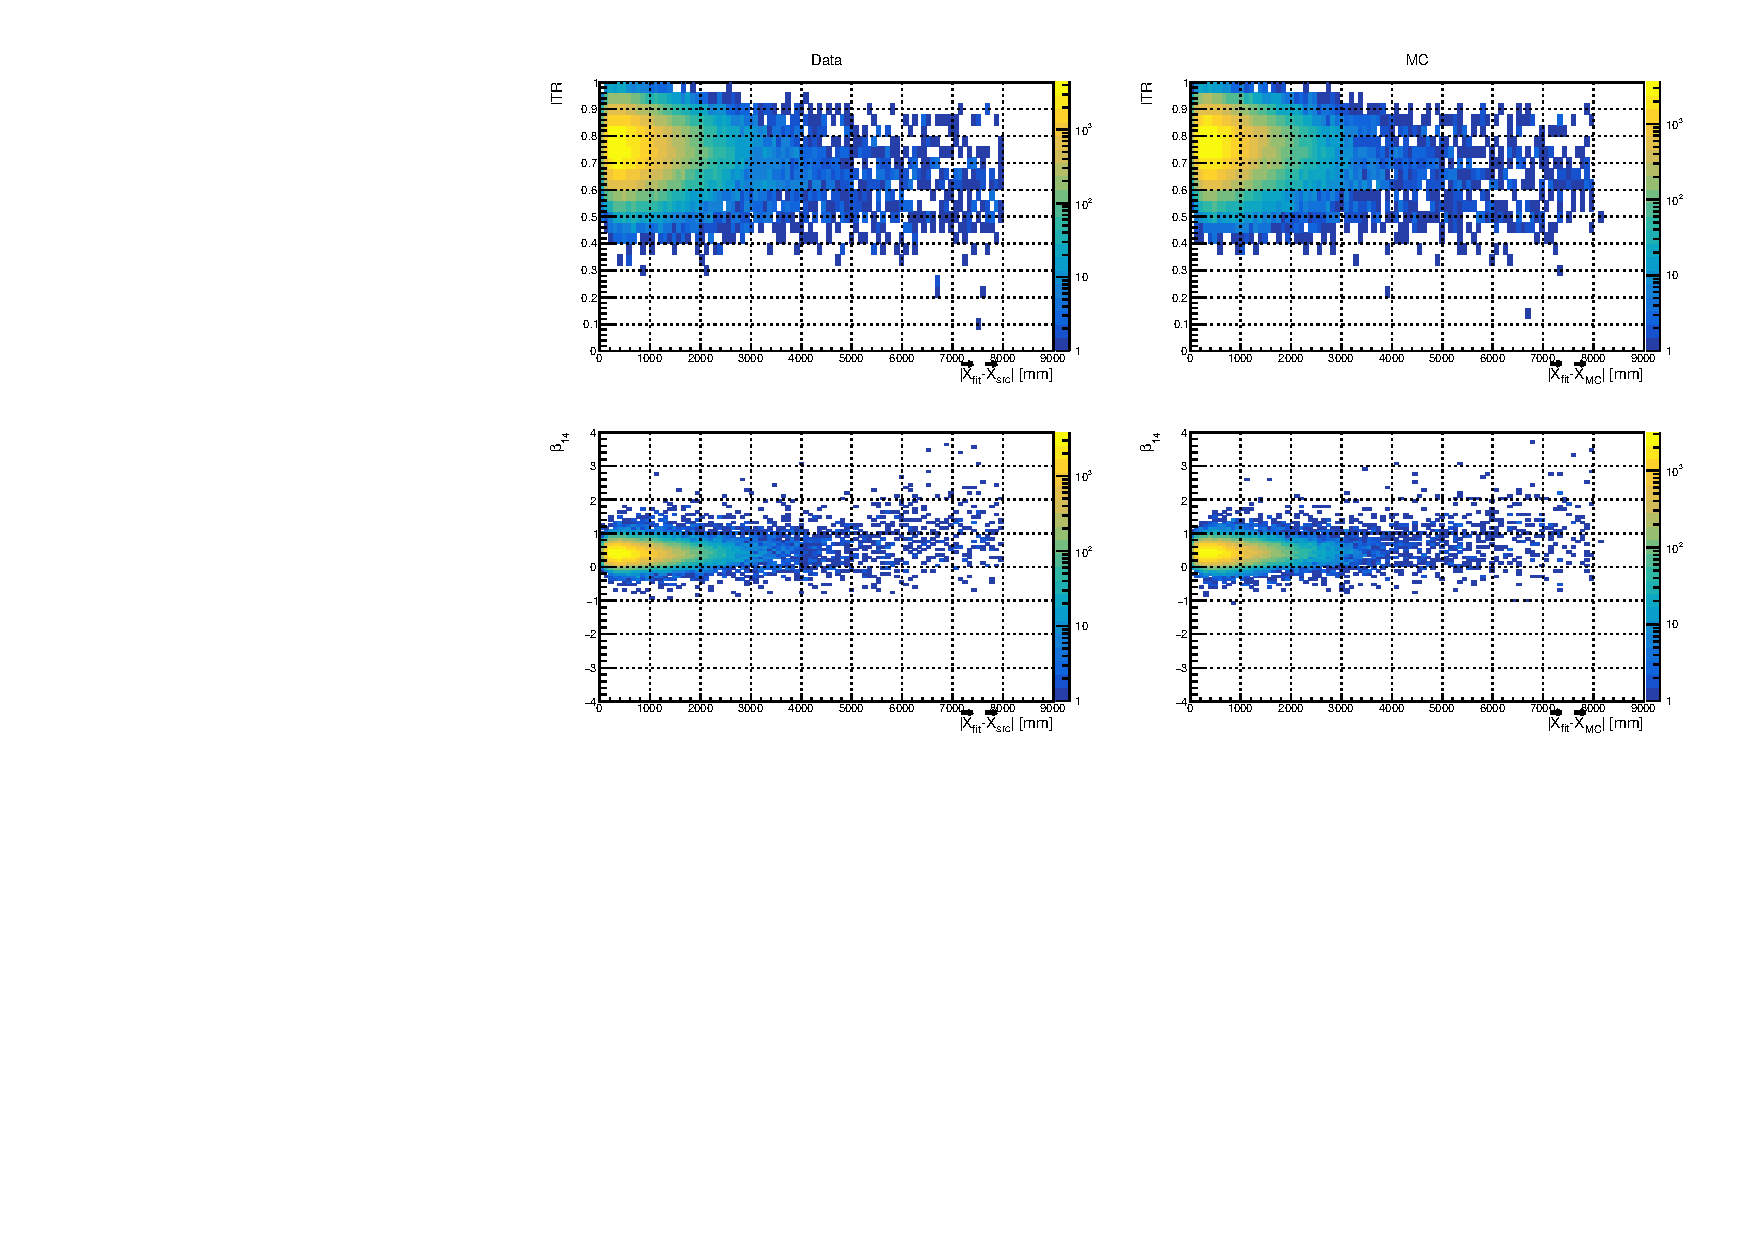
\includegraphics[width=14cm]{N16_107055_highLevelCuts.pdf}
	\caption[Position biases vs ITR and $\beta_{14}$ for the $^{16}$N central run 107055.]{Position biases vs ITR (top) and $\beta_{14}$ (bottom) for the $^{16}$N central run 107055. Left is MC and right is data. For the data, the offset of a reconstructed vertex was defined relative to the source position ($\vec{X}_{src}$). \label{n16_highLevelCut}}
\end{figure}


\section{Quality of Event Reconstruction Judged by $^{16}$N Calibration Scans in the Water Phase}

In this section, by analyzing the $^{16}$N data and corresponding simulations in the water phase, I extracted the resolution of the reconstruction algorithm for event position, direction, and energy. Then by comparing the data with the MC, the reconstruction systematics were evaluated.

To do these evaluations, a few cuts were applied to both the data and MC. Firstly, the level cuts (ITR$>0.55$, $-0.12<\beta_{14}<0.95$) were applied. For events having valid position, direction and energy reconstructions, further cuts on the reconstruction figure of merit (FoM) and source geometry (to be described in detail below) were applied, to ensure that the analyzed events were nicely reconstructed physics events caused by $\gamma$ particles (that originated in the source) interacting with the detector water.

\subsection{Position Reconstruction Evaluation}

The position figure of merit (posFoM) cuts mentioned in Sect.~\ref{sect:positionFoM} were applied on the reconstruction results. Fig.~\ref{posBiasVsFOM} shows the $scaleLogL$ with the position biases for the reconstructed events in the $^{16}$N central calibration run 107055. Results from both the data and the MC simulations are shown. For the MC case, the position biases are between the reconstructed positions and the true positions generated by the MC, $|\vec{X}_{fit}-\vec{X}_{MC}|$, while for the data, the biases are between the reconstructed positions and the source manipulator position, $|\vec{X}_{fit}-\vec{X}_{src}|$.

\begin{figure}
	\centering
	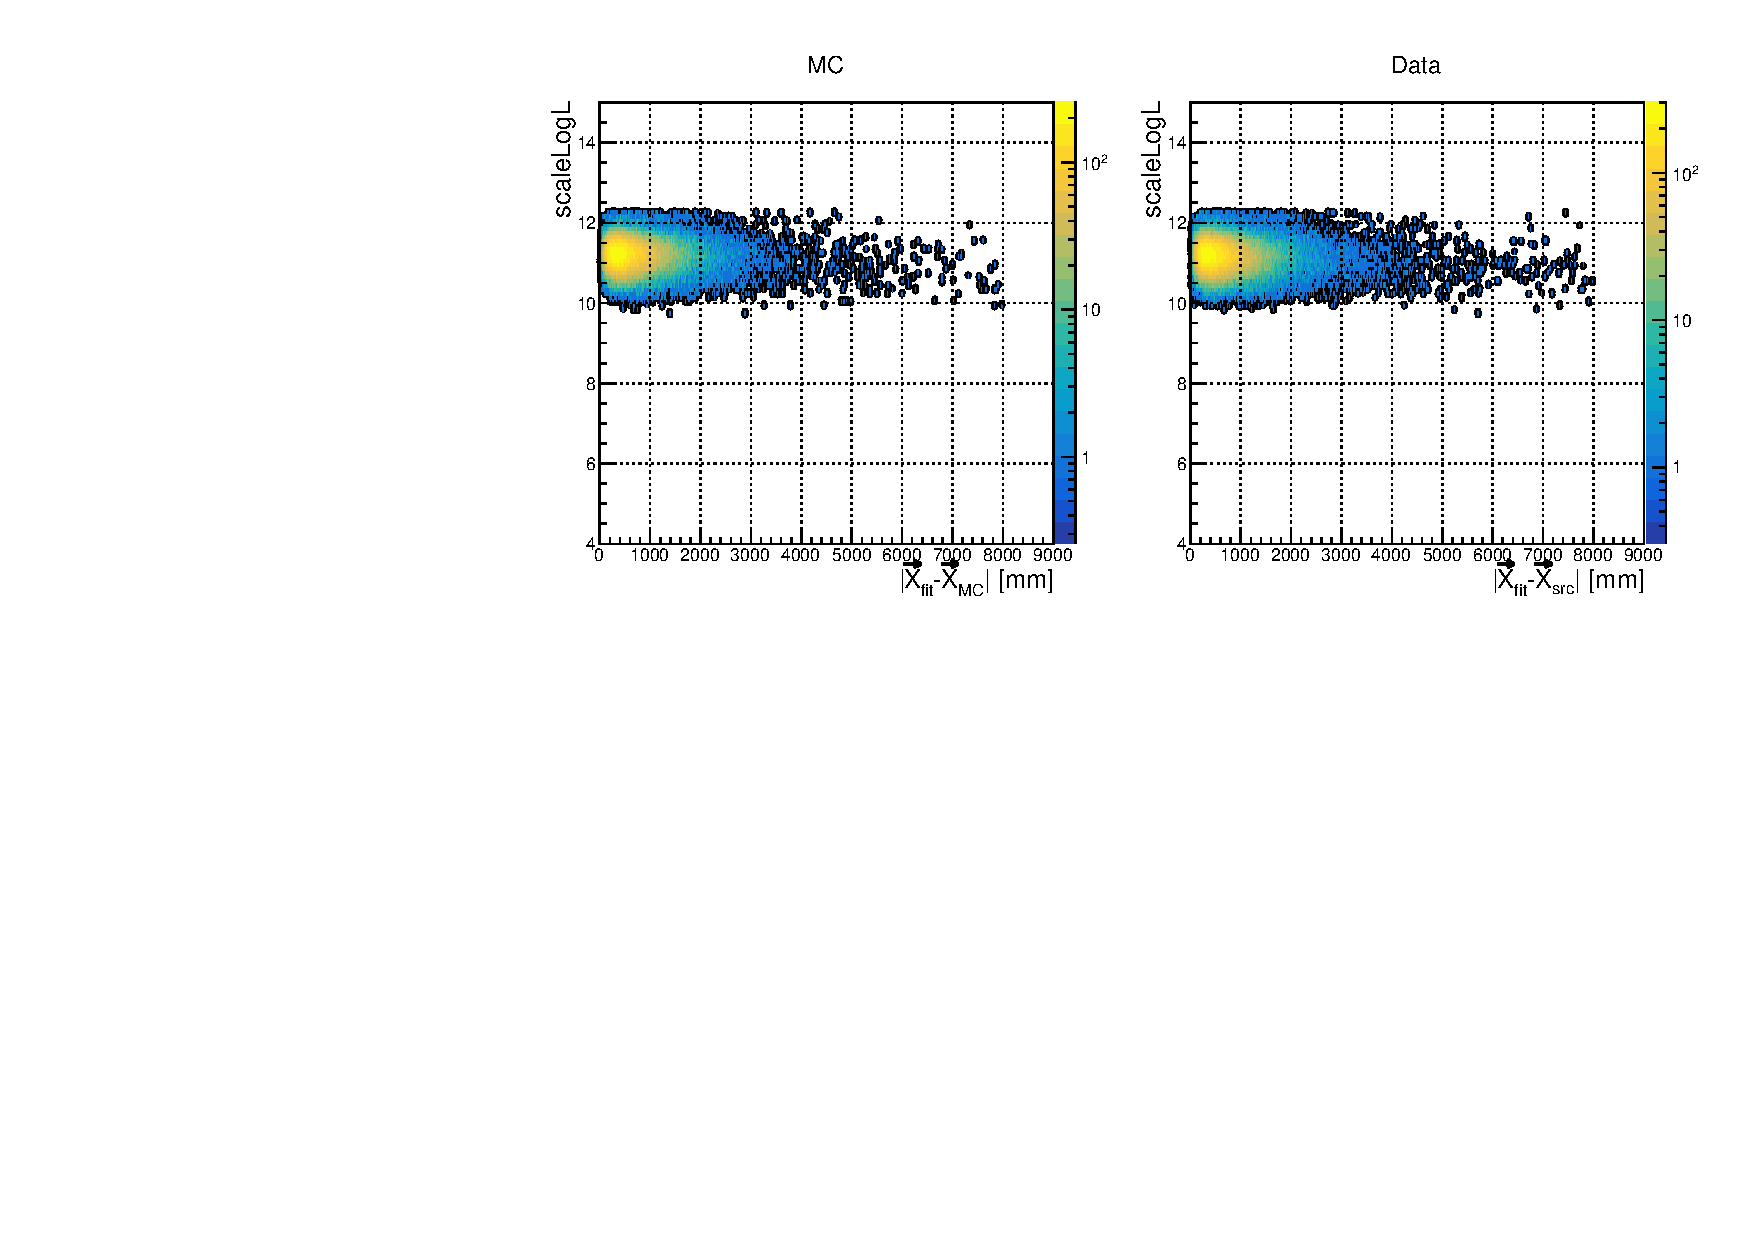
\includegraphics[width=13cm]{N16_107055_scaleLogLvsPosBias.pdf}
	\caption[Position biases vs $scaleLogL$ for the $^{16}$N central run 107055.]{Position biases ($|\vec{X}_{fit}-\vec{X}_{MC}|$) vs $scaleLogL$ for the $^{16}$N central run 107055. Left is MC and right is data. For the data, the offset of a reconstructed vertex was defined relative to the source position ($\vec{X}_{src}$).\label{posBiasVsFOM}}
\end{figure}

For the MC (data) case, about 0.035\% (0.043\%) of the total reconstructed events have large biases ($|\vec{X}_{fit}-\vec{X}_{MC}|>6000$ mm). A cut of $scaleLogL>10$ removes 96.0\% (97.3\%) of the events which have biases over 6000 mm, with a sacrifice of removing 0.012\% (0.016\%) of the total events.

Fig.~\ref{energyVsFOM} shows a relation between the $scaleLogL$ and the reconstructed energy ($E_{fit}$). Events with reconstructed energies below the water solar neutrino analysis threshold of 3.5~MeV ($E_{fit}<3.5~$MeV) are mostly coming from the U/Th isotopes, decays of Potassium and instrument noise \cite{waterunidoc}. Their lower energy (or NHits) negatively impacts the quality of position reconstruction because there are fewer hit PMTs providing information, so it is not unexpected that their $posFoM$ would be worse. In the MC (data) case, about 13.04 \% (12.89\%) of the events had $E_{fit}<3.5$~MeV. By applying a $scaleLogL>10$ cut, proportions of 0.10\% (0.09\%) of such events were removed.

\begin{figure}[!htb]
	\centering
	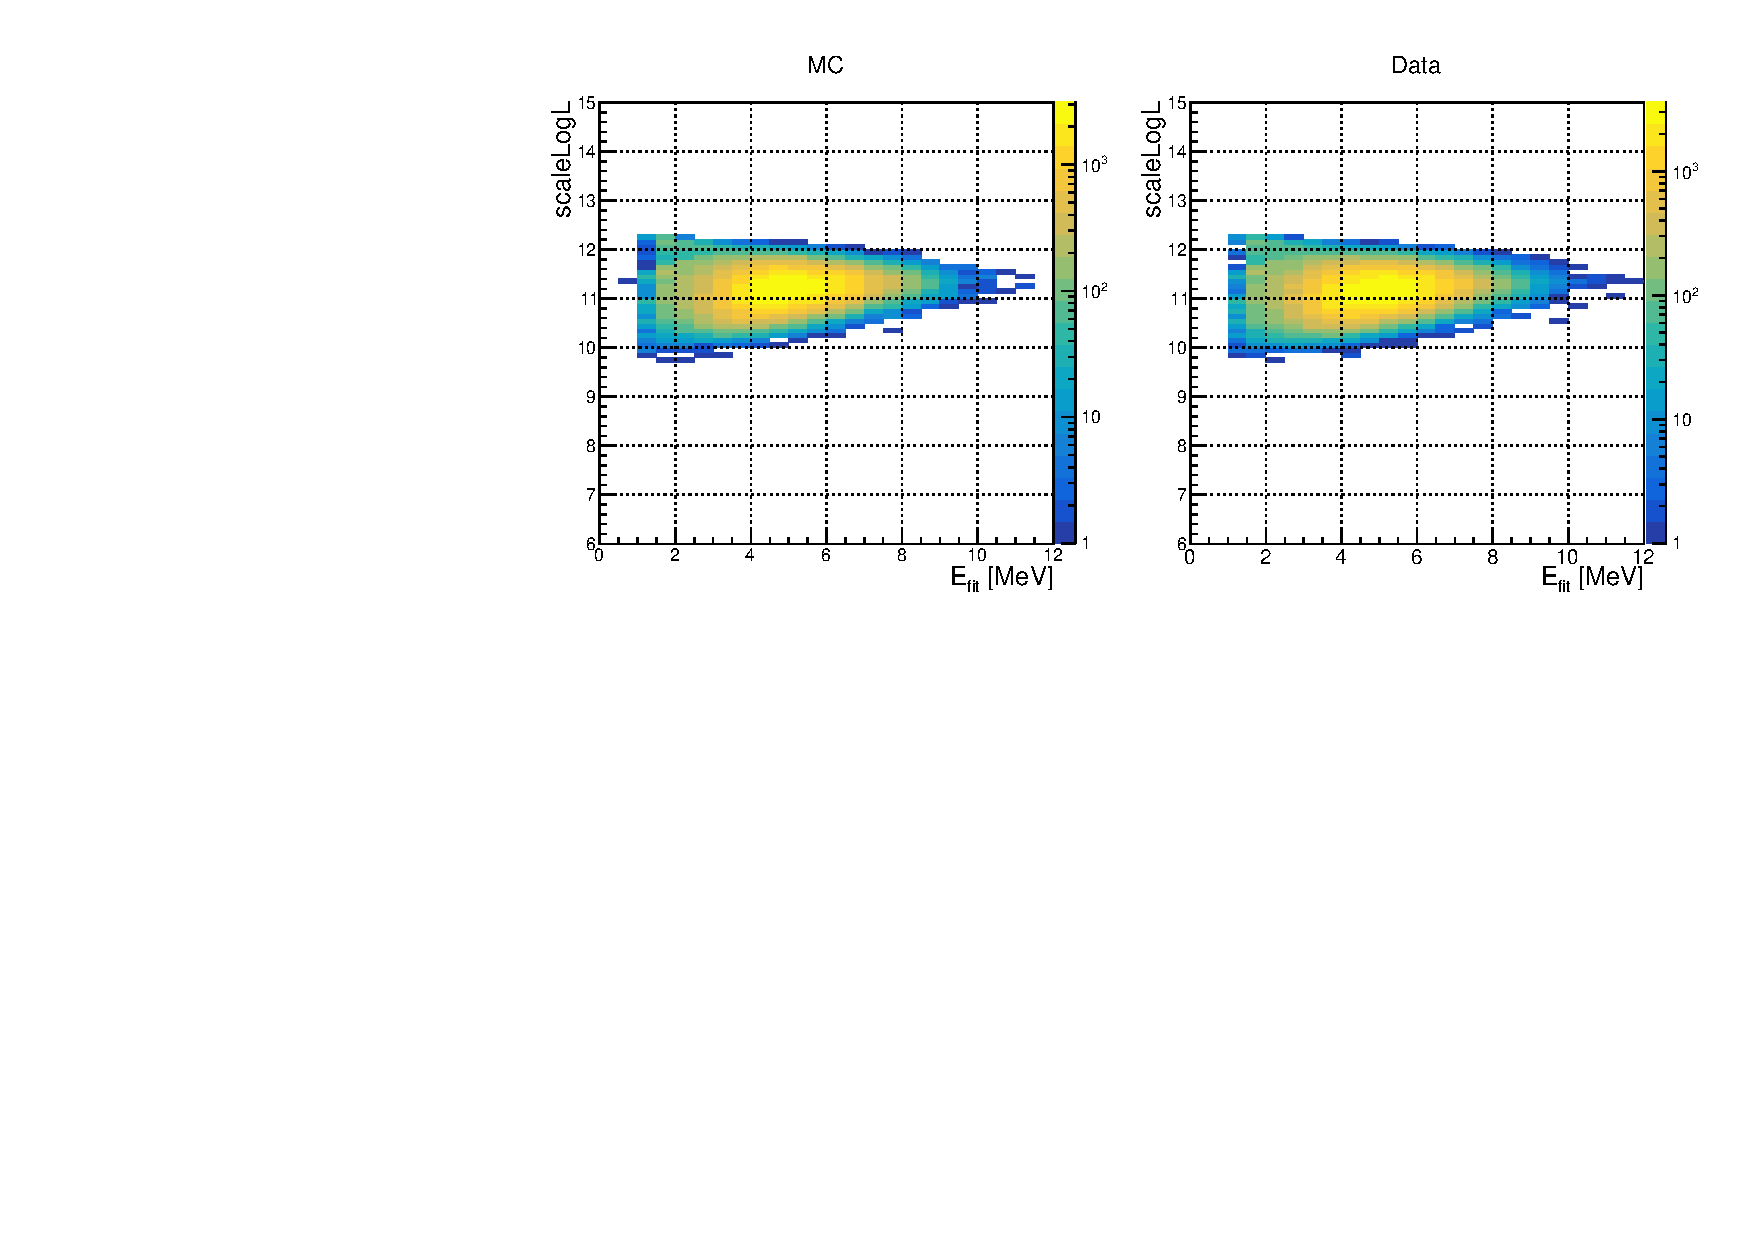
\includegraphics[width=13cm]{N16_107055_scaleLogLvsEnergy.pdf}
	\caption[Reconstructed energy vs $scaleLogL$ for the $^{16}$N central run 107055.]{Reconstructed energy vs $scaleLogL$ for the $^{16}$N central run 107055. Left is MC and right is data.\label{energyVsFOM}}

\end{figure}

As a summary, about 0.04\% of the events were poorly reconstructed (i.e. were mis-reconstructed) by the \texttt{MPW fitter}, resulting in a position error of over 6 meters. Applying a cut in $posFoM$ with $scaleLogL>10$ can remove over 96\% mis-reconstructed events. This $posFoM$ cut was used in the following direction and energy reconstruction evaluations.

\subsubsection{Position Resolution}\label{sect:positionResol}

A position resolution function is defined for the reconstructed electron position distribution \cite{boulay2004direct}:
\begin{equation}
R(x)=\frac{1-\alpha_e}{\sqrt{2\pi}\sigma_p}\exp{[-\frac{1}{2}(\frac{x-\mu_p}{\sigma_p})^2]+\frac{\alpha_e}{2\tau_p}\exp{[\frac{-|x-\mu_p|}{\tau_p}]}}\;,
\end{equation}
where $\alpha_e$ is the fractional exponential component, $\sigma_p$ is the Gaussian width (corresponding to the position resolution), $\mu_p$ is the Gaussian shift (corresponding to the position bias) and $\tau_p$ is the exponential slope (corresponding to the position distributions in tails).

The $\gamma$-rays emitted from the $^{16}$N source interact with the water in the detector mainly via Compton scattering, as shown in Fig.~\ref{N16centralDiagram}. The position distribution of the $\gamma$ interaction vertices (i.e. locations where electrons undergo scattering and are set in motion, producing Cherenkov light) encircles the source container, and extends out to a radius of about 2 meters. Fig.~\ref{hsx}, obtained from MC simulation, shows the spatial distribution $S(x)$ of the {\em first} $\gamma$-ray interaction positions (first Compton scatter) projected onto the $x$-axis. Therefore, the $^{16}$N source can be treated as an {\em electron} source having a known spatial distribution \cite{boulay2004direct}. For simplicity, in the following we always discuss the $x$ component of the position vector $\vec{X}$. 

\begin{figure}[!htb]
	\centering
	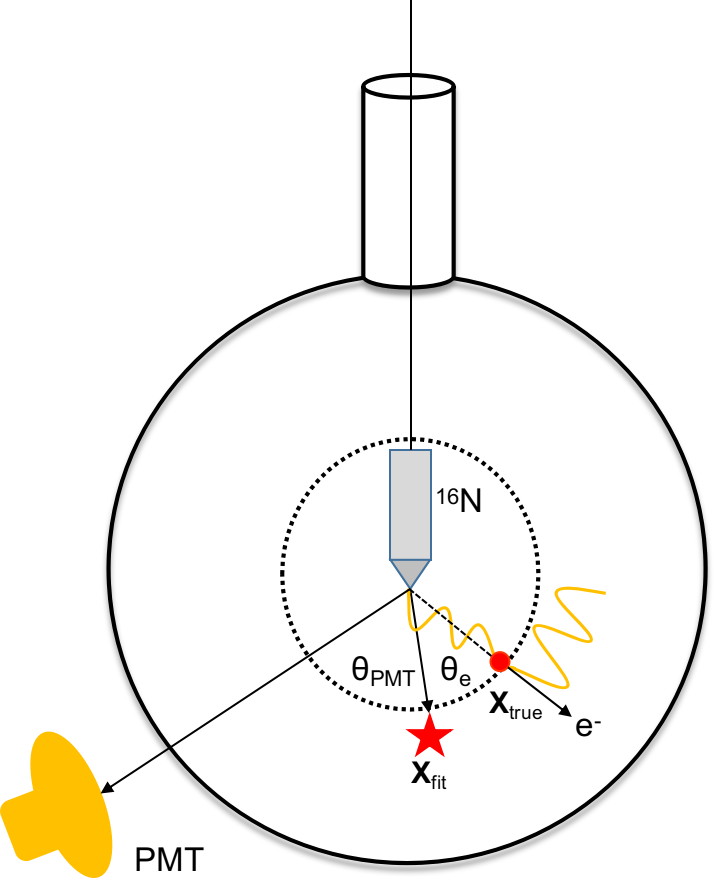
\includegraphics[width=8cm]{N16centralDiagram.png}
	\caption[Schematic of the $^{16}$N source.]{Schematic of the $^{16}$N source (not drawn to scale), showing the Compton scattering of a $\gamma$ emanating from the source. The radius of the dashed circle is about 2 m.	\label{N16centralDiagram}}
\end{figure}

\begin{figure}[!htb]
	\centering
	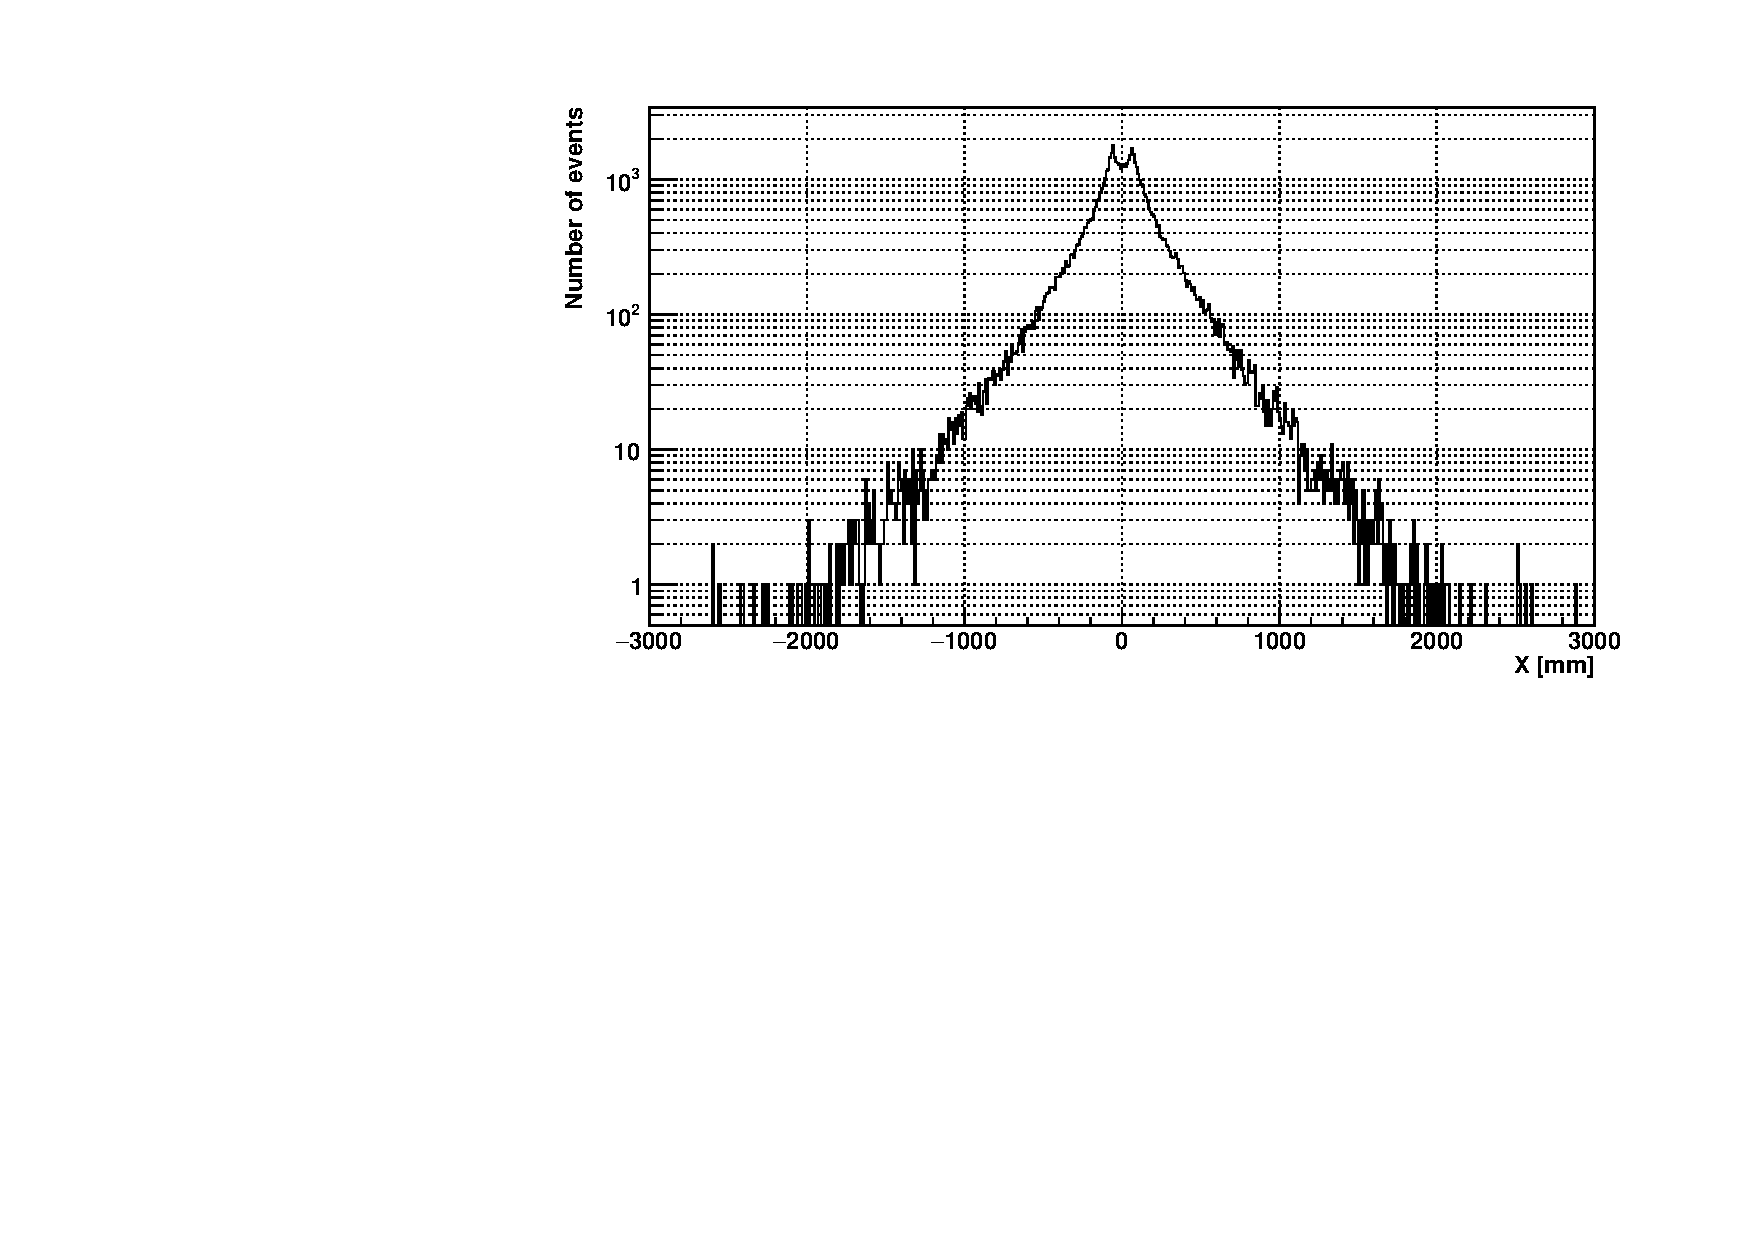
\includegraphics[width=12cm]{sx.pdf}
	\caption[Spatial distribution of {$^{16}$}N $\gamma$-ray's first interaction positions, projected onto the $x$-axis.]{Spatial distributions of {$^{16}$}N $\gamma$-ray's first interaction position, projected onto the $x$-axis, obtained from the \texttt{RAT} simulations. The double-peak structure is due to the wall of the stainless steel container of the $^{16}$N source.\label{hsx}}
\end{figure}

The spatial distribution function $N_{R}(x)$ for electrons from the $^{16}$N calibration source can be described by the convolution of the position resolution function with $S(x)$ \cite{boulay2004direct},
\begin{equation}
N_{R}(x)=\int^{+\infty}_{-\infty} S(x) \, R(x_{fit} - x) \, dx \; .
\end{equation}

The values of $N_{R}(x)$ can be calculated bin by bin from histograms of $S(x)$ and $R(x)$ extracted from the MC or data, 
\begin{equation}
N_R(x_i)=\sum_{x_i=-\infty}^{+\infty}S(x_i) \, R(x_{fit}^i-x_i) \; .
\end{equation}

Then the $\chi^2$ statistic is calculated, 
\begin{equation}
\chi^2=\sum^{N_{bins}}_{i=0}[\frac{N_R(x_{fit}^i)-N_R^{fit}(x_{fit}^i)}{\sigma_i}]^2 \; ,
\end{equation}
where $N_R^{fit}$ is a trial fit to the $N_R$ obtained by tuning $(\alpha_e,\mu_p,\sigma_p,\tau_p)$, and $\sigma_i$ is obtained from the bin width of the histograms. By minimizing $\chi^2$, the parameters $(\alpha_e,\mu_p,\sigma_p,\tau_p)$ of the resolution function, and a best $N_R^{fit}$, were obtained. Fig.~\ref{fig:posresol} shows a comparison of the reconstructed $x$ position of {$^{16}$}N events between data and MC. The reconstructed position distributions were fitted with $N_R^{fit}$.

\begin{figure}
	\centering
	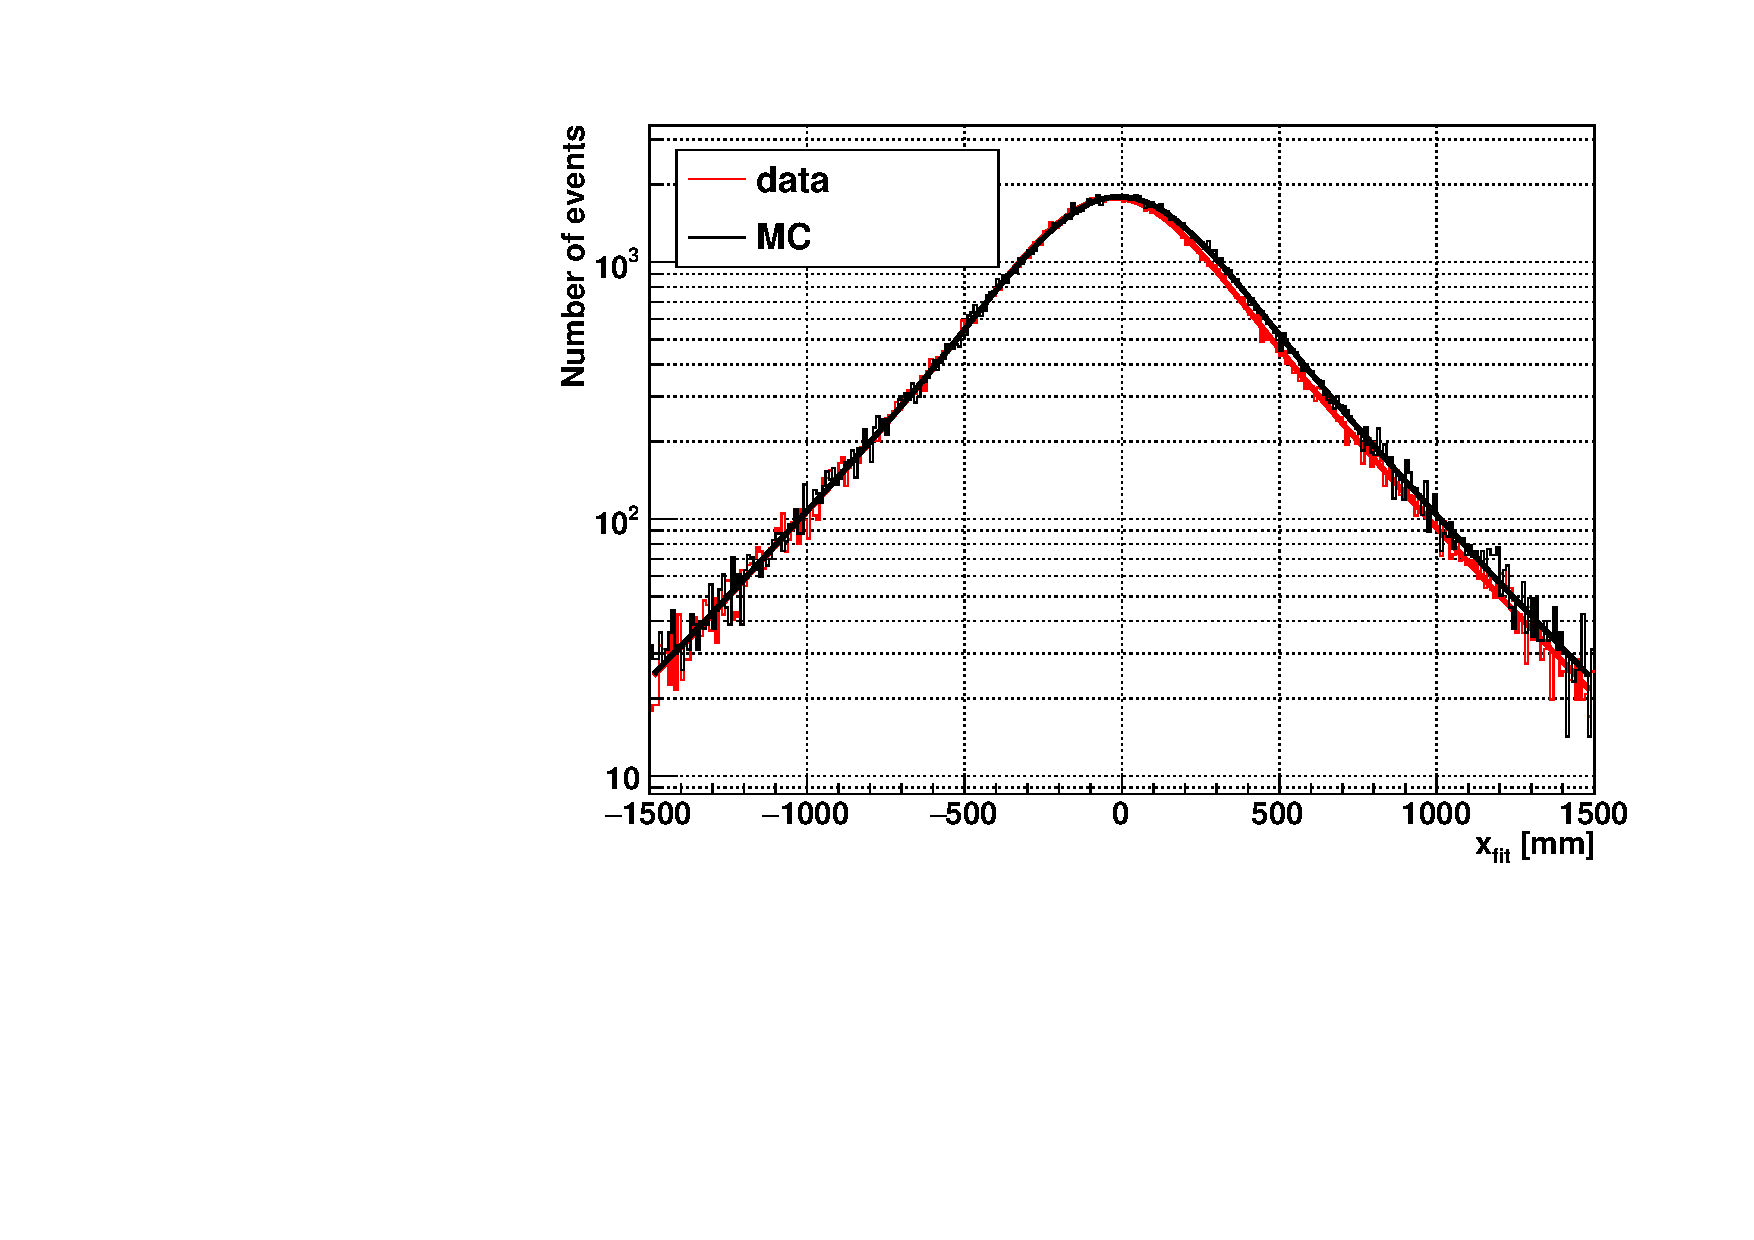
\includegraphics[width=140mm]{posResol.pdf}
	\caption[Distributions of the reconstructed position projected onto the $x$-axis.]{Distributions of the reconstructed position projected onto the $x$-axis, obtained from the SNO+ {$^{16}$}N central run data (red) and MC (black). The distributions are fitted with $N_R^{fit}$ (red and black lines).	\label{fig:posresol}}
\end{figure}

Table~\ref{tab:posresol} summarizes the values of position resolution parameters (for the $x$-axis) obtained from data and MC of {$^{16}$}N calibration runs at the detector center.
\vspace{1mm}
\begin{table}[ht]
	\centering
	\caption{Position resolution parameters for the \texttt{MPW fitter} ($x$-axis).}
	\label{tab:posresol}
	\begin{tabular}{ccccc}
		\toprule
		MPW fitter & $\alpha_e$ & $\sigma_P$ (mm) & $\tau_P$ (mm)& $\mu_P$ (mm)\\
		\hline 
		data& 0.58$\pm$0.04 & 175.8$\pm$3.8 & 288.0$\pm$5.7 & -28.8$\pm$1.0\\
		\hline 
		MC & 0.51$\pm$0.05 & 195.2$\pm$3.3 & 298.4$\pm$6.1 & -10.9$\pm$1.0\\
		\bottomrule
	\end{tabular}
\end{table}
\vspace{1mm}

\subsubsection{Position Systematics}

To evaluate the position uncertainties, the MC and data runs of the $^{16}$N internal scans along ($x, y, z$) axes were taken to evaluate the $(x, y, z)$ position uncertainties respectively (the runs are listed in Table~\ref{table:n16scanTable_zscan} to ~\ref{table:n16scanTable_xscan}. Three neck runs in the $z$-scan were not used). The high-level cuts mentioned earlier, as well as the $E_{fit}>3.5$~MeV and $scaleLogL>10$ cuts, were applied. The fit range was set as $[X_\mathrm{source}-2000, X_\mathrm{source}+2000]$~mm, where $X=(x,y,z)$ for the scans along $(x,y,z)$ axes respectively. This is because, recall, most of the source $\gamma$'s have their first Compton scatter -- knocking an $e^{-}$ into motion -- within that distance from the source. If the value of $(X-2000)~$mm was smaller than -6000~mm, it was set to -6000~mm; if the $(X+2000)~$mm was larger than 6000~mm, it was set to +6000~mm. This was used to remove the AV effects, mainly the AV lensing and the material boundaries which distort the reconstruction performances, as mentioned in Chapter 4.

The position resolution function was first fitted with four free parameters, $(\alpha_e,\mu_p$, $\sigma_p$, $\tau_p$). The average values of $\alpha_e$ and $\tau_p$ were calculated from all the scan runs used here and then, to simplify the calculation in propagating systematics, those average values\footnote{Using fixed values for ($\alpha_e$, $\tau_p$) is justified by the fact that these parameters in principle can be viewed as corrections to the spatial distribution of the $\gamma$'s ($S(x)$) that would not depend on position \cite{waterunidoc}.} were assigned as constant values: $\alpha_e=0.5288$ (0.5375) for the MC (data) and $\tau_p=271.738$ (263.735) for the MC (data). With the fixed values of $\alpha_e$ and $\tau_p$, both the data and the MC were refitted to optimize $\mu_p$ and $\sigma_p$ only. 

Fig.~\ref{MPWscanXYZResols} shows the fitted results for $\mu_P$ and $\sigma_P$ along the $(x, y, z)$-axes scans respectively. For the sake of simplicity, for the $x$-scan case, only the $x$-axis results ($\mu_{P,x},\sigma_{P,x}$) are shown here. Similarly, only the $\mu_{P,y}$ and $\sigma_{P,y}$ ($\mu_{P,z}$ and $\sigma_{P,z}$) are shown for the $y$-scan ($z$-scan). The relative differences discussed later consider all three axes.

\begin{figure}
	\centering
	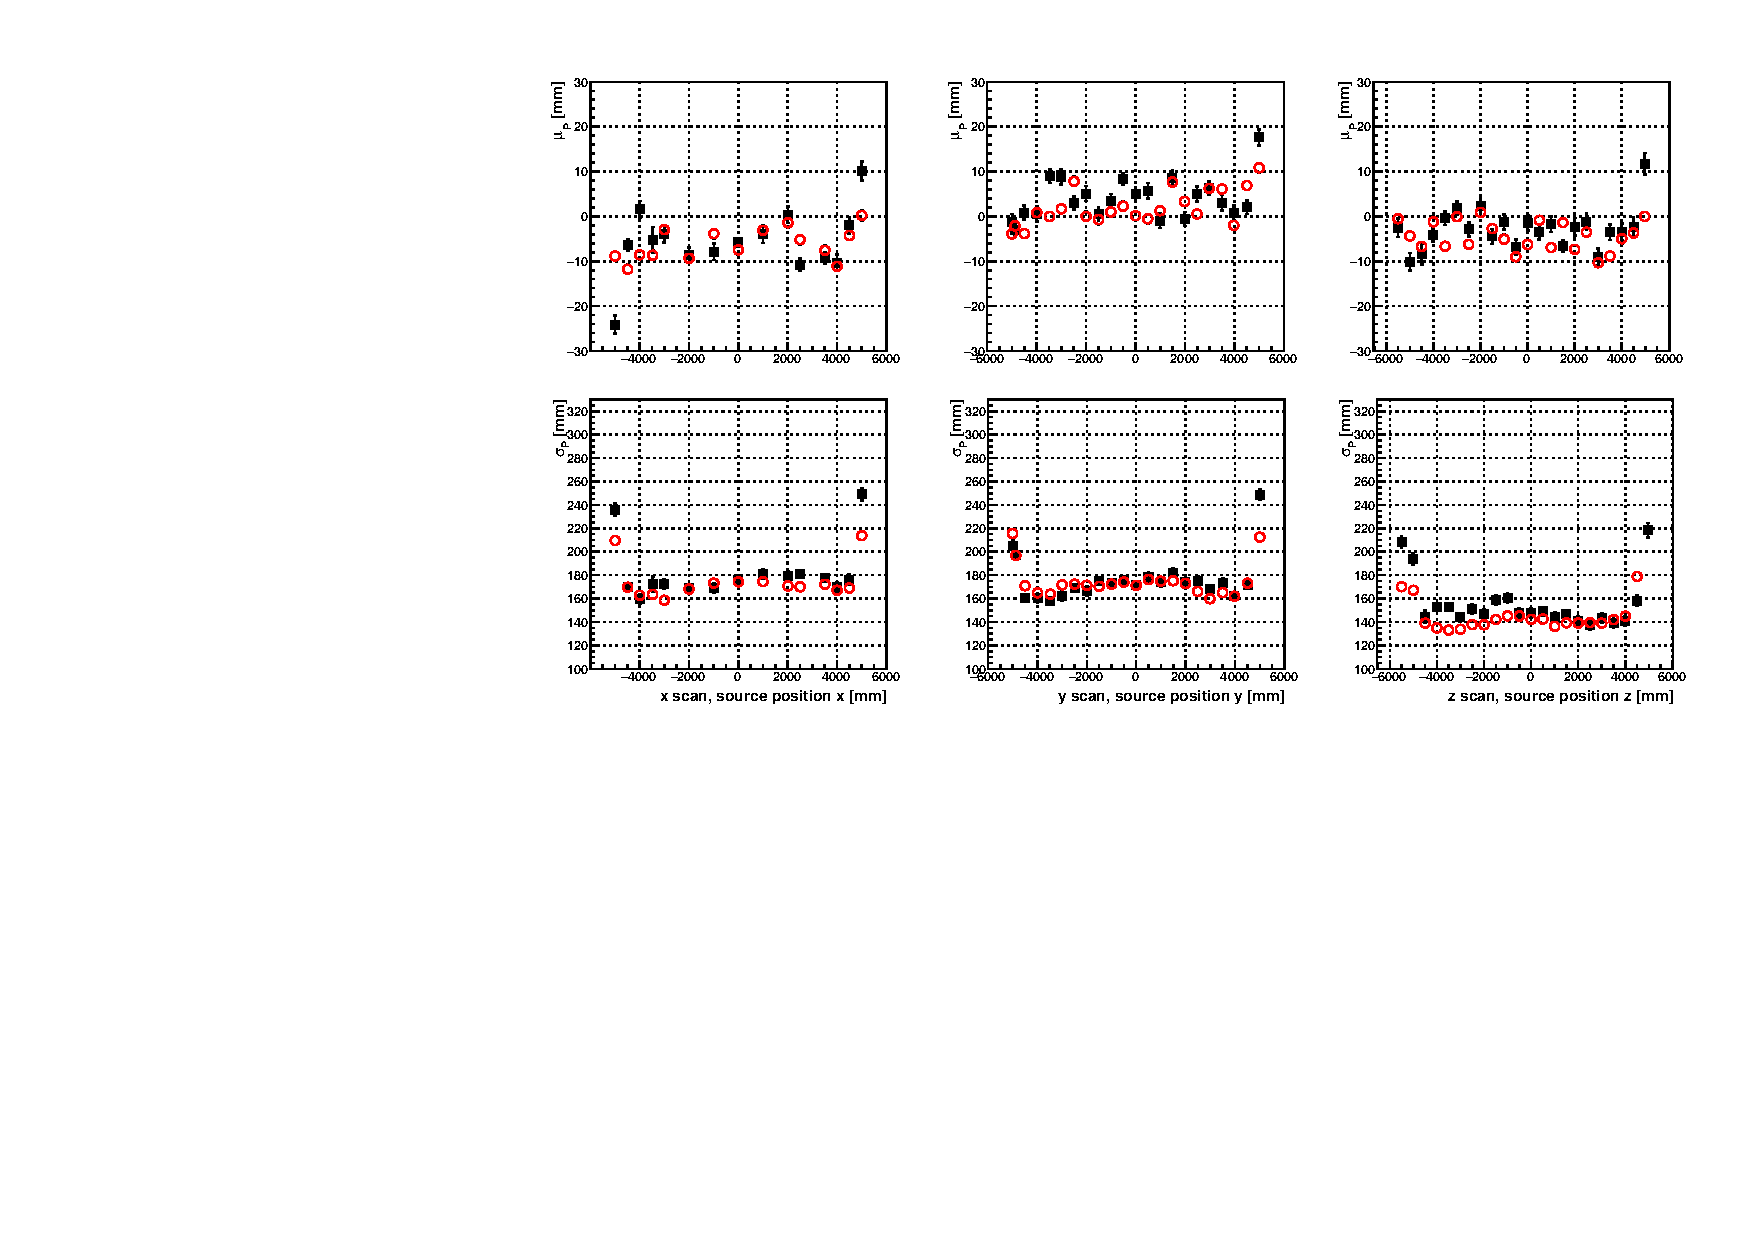
\includegraphics[width=16cm]{N16_rat6176_muPandSigmaP_xyzScans.pdf}
	\caption[The fitted values of $\mu_P$ and $\sigma_P$ along $x$, $y$ and $z$-scans.]{The fitted values of $\mu_P$ (top) and $\sigma_P$ (bottom) along $x$ (left), $y$ (middle) and $z$ (right) scans. The source positions in each set of scans are projected onto $(x, y, z)$ axes respectively. The MC results (red circles) are compared with the data (black boxes).	\label{MPWscanXYZResols}}
\end{figure}

Fig.~\ref{MPWscanXYZResols} shows that the resolution for vertex reconstruction is generally better for the MC simulations than for the detector data. This is not unexpected, because of the non-uniformities of the detector in realistic situations (as opposed to the idealizations inherent in the MC simulation) \cite{waterunidoc}. Also, when the source is close to the AV or at the ends of the axes, the Gaussian shift $\mu_P$ becomes large and the resolution worsens, which causes the difference between the MC and data to become large.

To quantify the discrepancies between the MC and data, a relative difference of $\sigma_p$ between the MC and data is defined as \cite{waterunidoc}

\begin{equation}
\sigma_{p,\delta}\equiv\sqrt{\sum_i|(\sigma^{data}_{P,i})^2-(\sigma^{MC}_{P,i})^2|}~~(i=x,y,z)\; ,
\end{equation}

Fig.~\ref{pos_relative_sigma_biasesVsPositions} shows that $\sigma_{p,\delta}$ varies along the internal ($x, y, z$)-axis scans. All the $\sigma_p$ values are smaller than $190~$mm, except for that with the source at $z=4973.567~$mm (run 106979) and (therefore) in proximity to the neck of the AV, whose presence probably is responsible for the anomaly. Looking at the pattern on Fig.~\ref{pos_relative_sigma_biasesVsPositions} we see that $\sigma_p$ is larger (worse) when the source is close to the AV (i.e. at the end of the position axes) and that when the source is close to the {\em center} of the AV, the differences are below $100~$mm.

\begin{figure}[!htb]
	\centering
	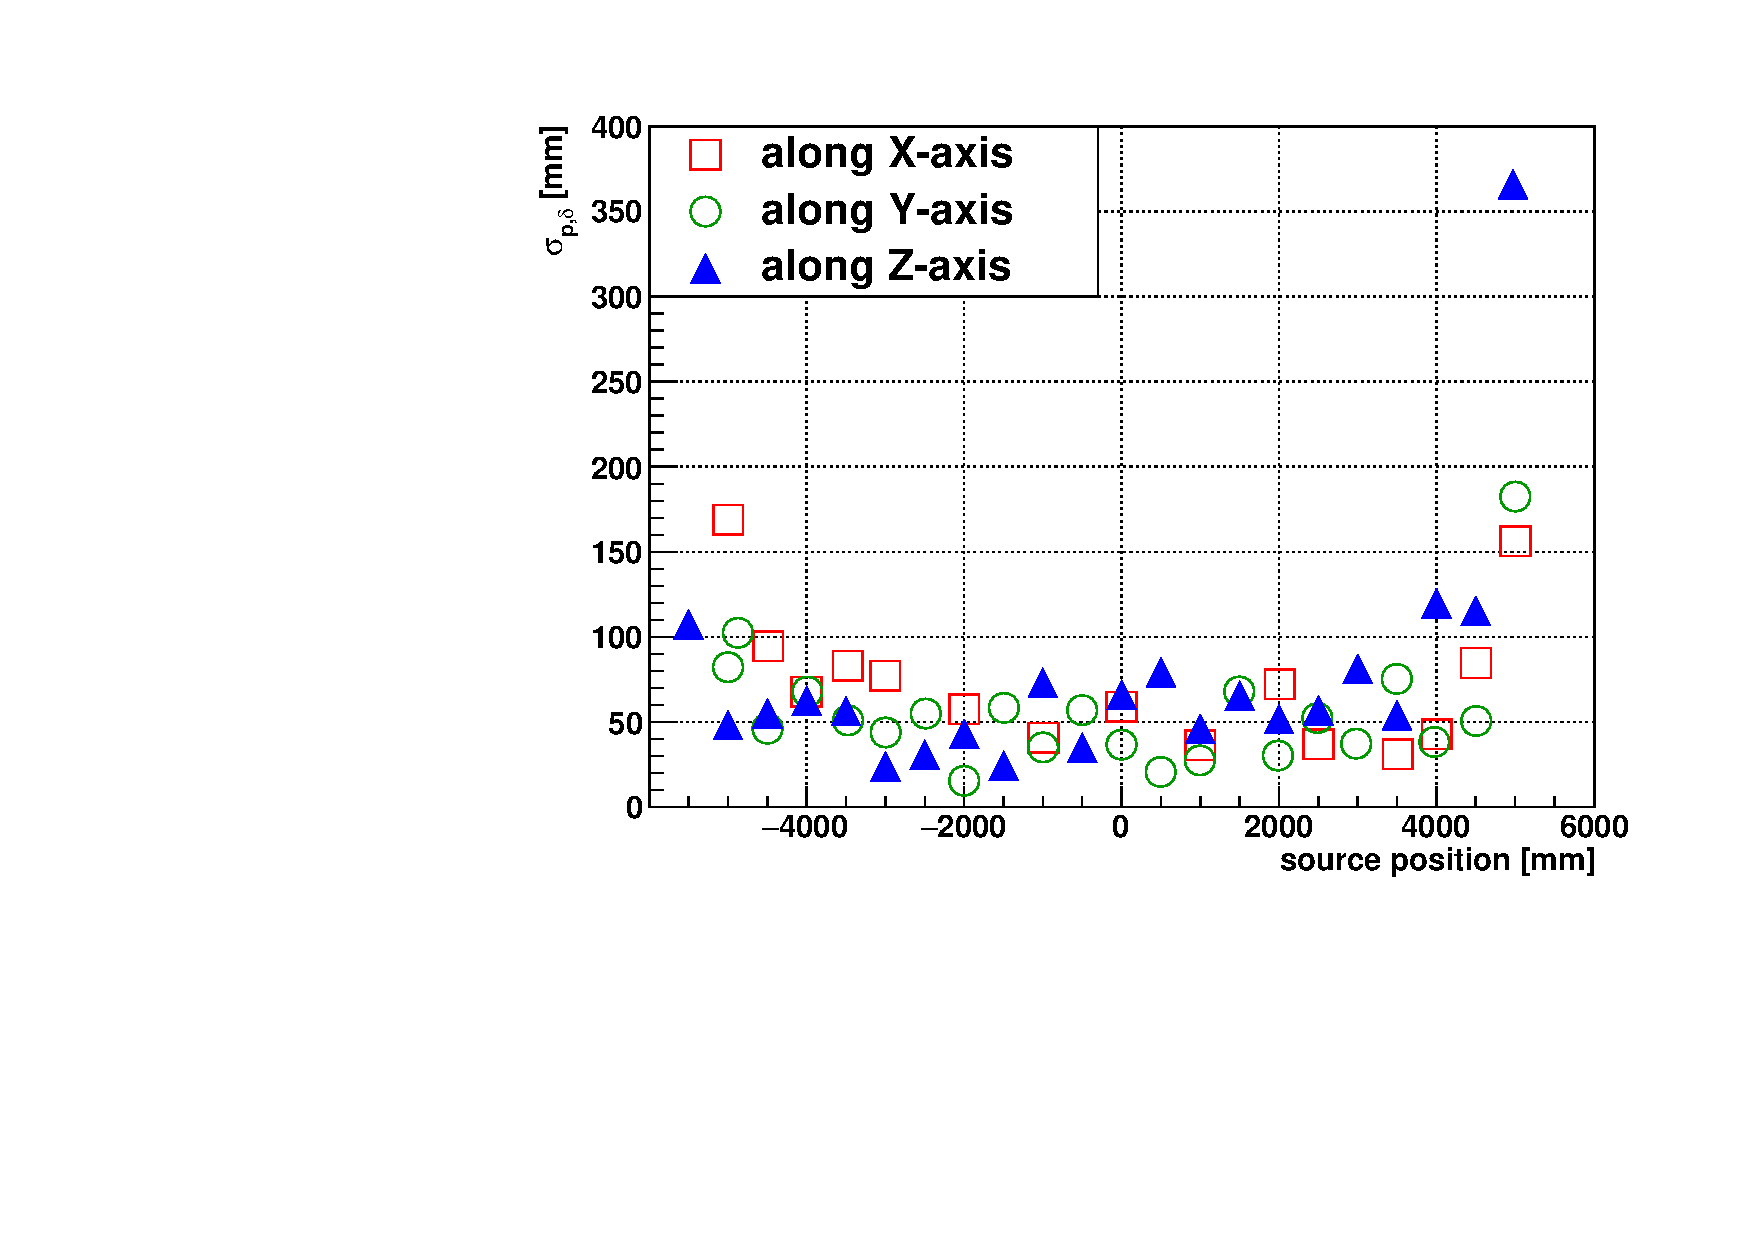
\includegraphics[width=15cm]{N16_6176_pos_sigmaP_data_mc.pdf}
	\caption[Relative differences of $\sigma_P$ ($\sigma_{p,\delta}$) as a function of the $^{16}$N source position.]{Relative differences of $\sigma_P$ ($\sigma_{p,\delta}$) as a function of the $^{16}$N source position. For simplicity, the corner scans are not shown in this figure. The red squares represent the results from the $x$-scan runs; green circles represent the $y$-scan runs and the blue triangles represent the $z$-scan runs.	\label{pos_relative_sigma_biasesVsPositions}}

\end{figure}

As listed in Table~\ref{vertexResolsSys}, the averages and the standard deviations of $\sigma_{p,\delta}$ were taken as the resolution systematics for the $(x, y, z$)-axes respectively. To smear the position results, a Gaussian distribution $\mathcal{N}(0,\delta)$ was convolved with positions. The listed values for the standard deviation ($\delta$) of this Gaussian were used to smear the positions.
\begin{table}[ht]
	\centering
	\caption[Systematic uncertainties of the \texttt{MPW fitter} for position on $(x,y,z)$-axes.]{Systematic uncertainties of the \texttt{MPW fitter} for position on $(x,y,z)$-axes.	Unit: mm.\label{vertexResolsSys}}
	\vspace{3mm}
	\begin{tabular*}{140mm}{c@{\extracolsep{\fill}}ccc}
		\toprule
		axis & systematic uncertainties & systematic to be applied ($\delta$) &smearing\\
		\hline 
		$x$  & $73.89\pm39.71$ & 113.6 & $x+\mathcal{N}(0,\delta)$\\
		$y$  &  $56.03\pm34.96$ & 90.99 & $y+\mathcal{N}(0,\delta)$\\
		$z$   & $75.47\pm70.09$ & 145.56& $z+\mathcal{N}(0,\delta)$\\
		\bottomrule
	\end{tabular*}
\end{table}

To quantify the vertex shifts between the MC and data, values of vertex shifts: $\mu_{P,\delta}\equiv\mu_P(data)-\mu_P(MC)$ were calculated for the ($x, y, z$) scans. Fig.~\ref{fig:verteshitfs} shows these results.
\begin{figure}[!htb]
	\centering
	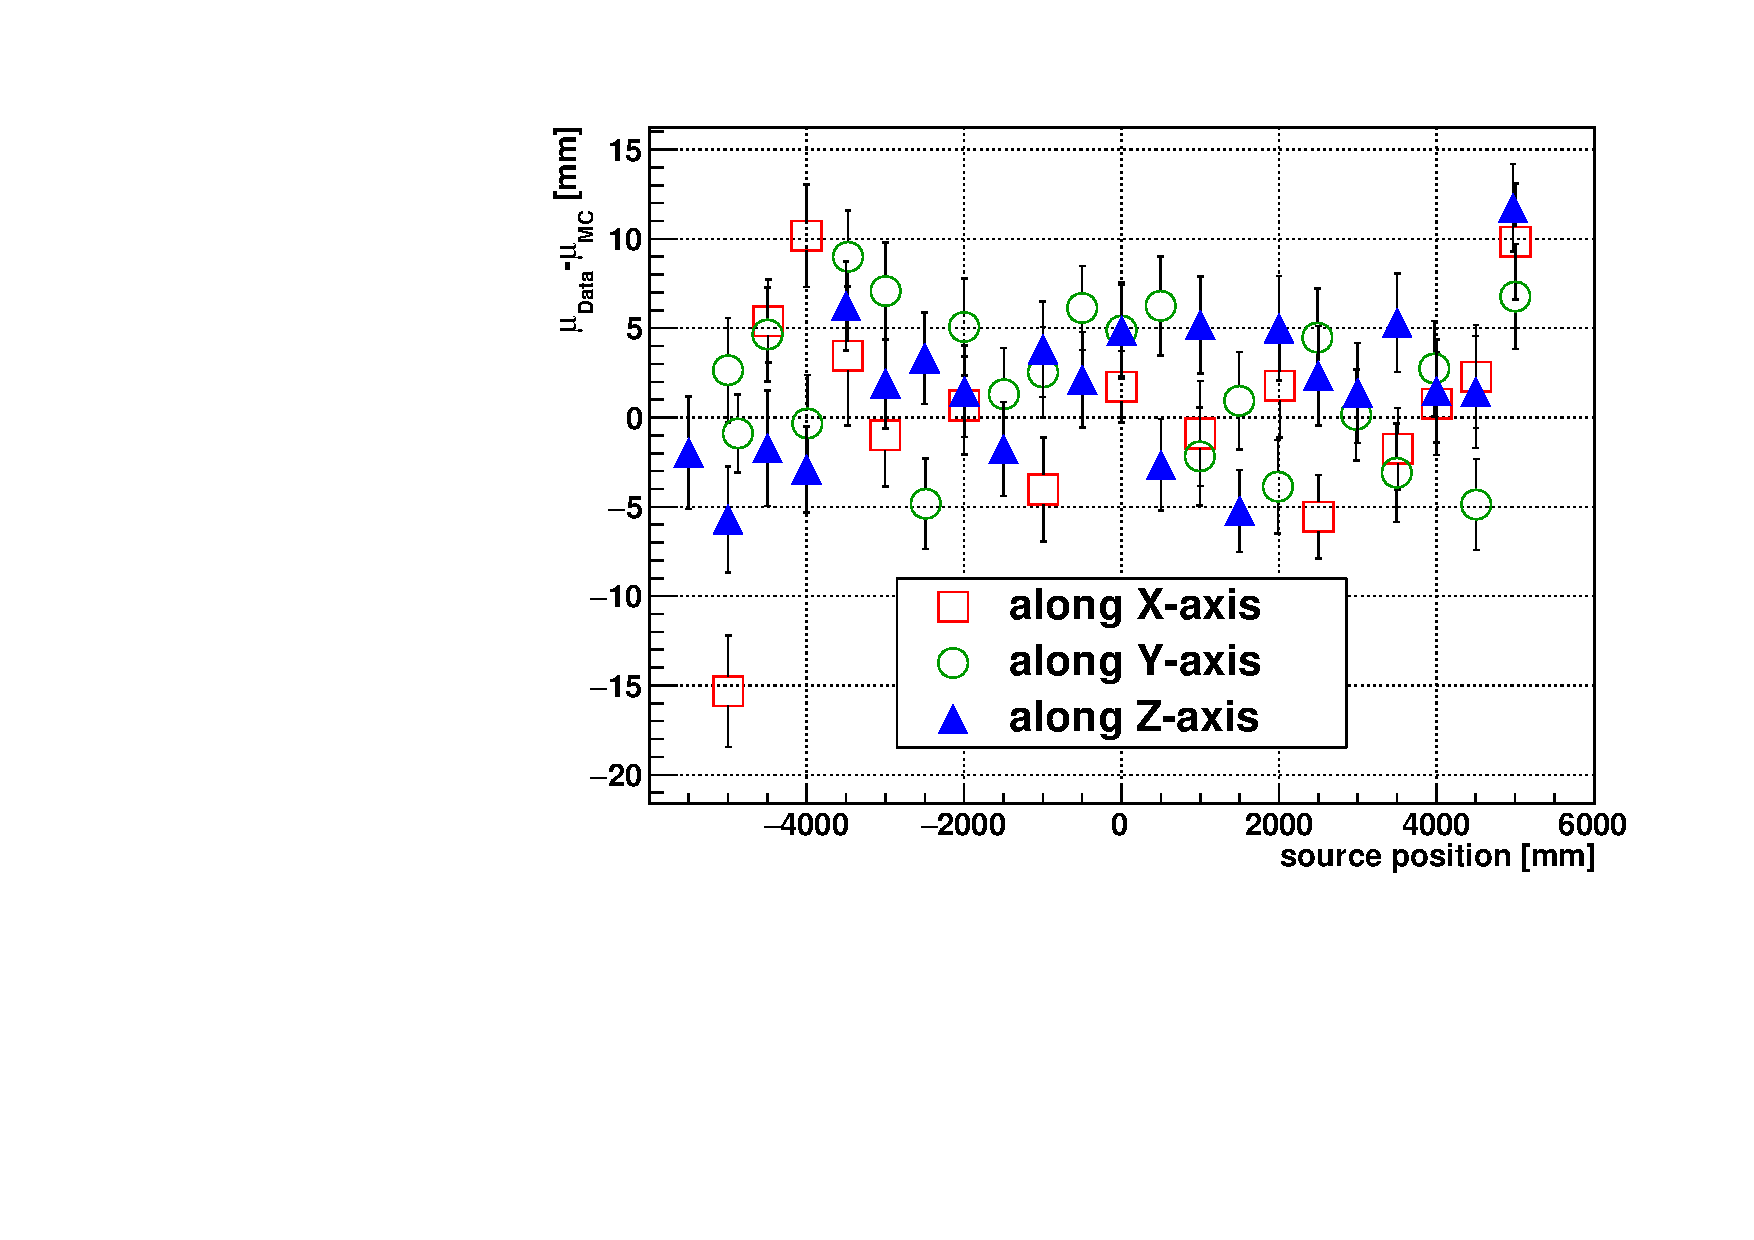
\includegraphics[width=15cm]{N16_rat6176_vertexShift_xyzScans.pdf}
	\caption[Vertex shifts of $\mu_P$ ($\mu_{p,\delta}$) as a function of the $^{16}$N source position.]{Vertex shifts of $\mu_P$ ($\mu_{p,\delta}$) as a function of the $^{16}$N source position. For simplicity, the corner scans are not shown in this figure. The red squares represent the results from the $x$-scan runs; green circles represent the $y$-scan runs and the blue triangles represent the $z$-scan runs.\label{fig:verteshitfs}}
\end{figure}

In Table~\ref{vertexShifts}, the averages and the standard deviations of $\mu_{P,\delta}$ were taken as the vertex shifts for ($x, y, z$)-axes. To smear the position results, the $(x,y,z)$ values were shifted up or down by adding positive or negative values. The values on each axis were shifted independently. For example, the x shift-up is $(x,y,z)\to(x+6.48,y,z)$ mm; the z shift-down is $(x,y,z)\to (x,y,z-4.82)$ mm.

\begin{table}[ht]
	\centering
	\caption{Vertex shifts for the reconstructed positions on ($x, y, z$) axes. Unit: mm. \label{vertexShifts}}
	\vspace{3mm}

	\begin{tabular*}{120mm}{c@{\extracolsep{\fill}}cccc}
		\toprule
		axis & vertex shift  & systematic to be applied ($\delta$) &smearing\\
		\hline 
		$x$ shift &  0.50$\pm$5.98 & +6.48/-5.98 & $x+\delta$\\	
		$y$ shift  & 2.02$\pm$4.11 & +6.13/-4.11 & $y+\delta$\\
		$z$ shift & 1.89$\pm$4.82 & +6.71/-4.82 & $z+\delta$\\
		\bottomrule
	\end{tabular*}
\end{table}

\subsubsection{Vertex Scale Uncertainties}

In addition to the vertex shifts mentioned previously, the vertex scale is defined as a linear scale factor between the fitted positions of the data and the MC,
\begin{equation}
x^{data}_{fit}-x^{MC}_{fit}=\mu^{data}_{P,x}-\mu^{MC}_{P,x}=\Delta + \beta \; x^{MC}_{fit} \; .
\end{equation}
Since $x^{data}_{fit}=\Delta + (1+\beta) \; x^{MC}_{fit}$, if the vertex scale factor is defined $\alpha\equiv 1+\beta$ then $x_{data}=\alpha x_{MC}$. %%%% needs to be clearified

To obtain $\alpha$, the results in Fig.~\ref{fig:verteshitfs} were fitted with linear functions: $shifts = p_0+p_1 \; x_\mathrm{src}$ (where $x_\mathrm{src}$ is the source position), as shown in Fig.~\ref{fig:vertexScale}. %John: {red}(What do you mean by `shifts'? If it is a specific variable, please give the variable's name. If it is a new variable, can a nicer symbol be used?){red}

\begin{figure}
	\centering
	\subfigure[$^{16}$N x-scan runs.]{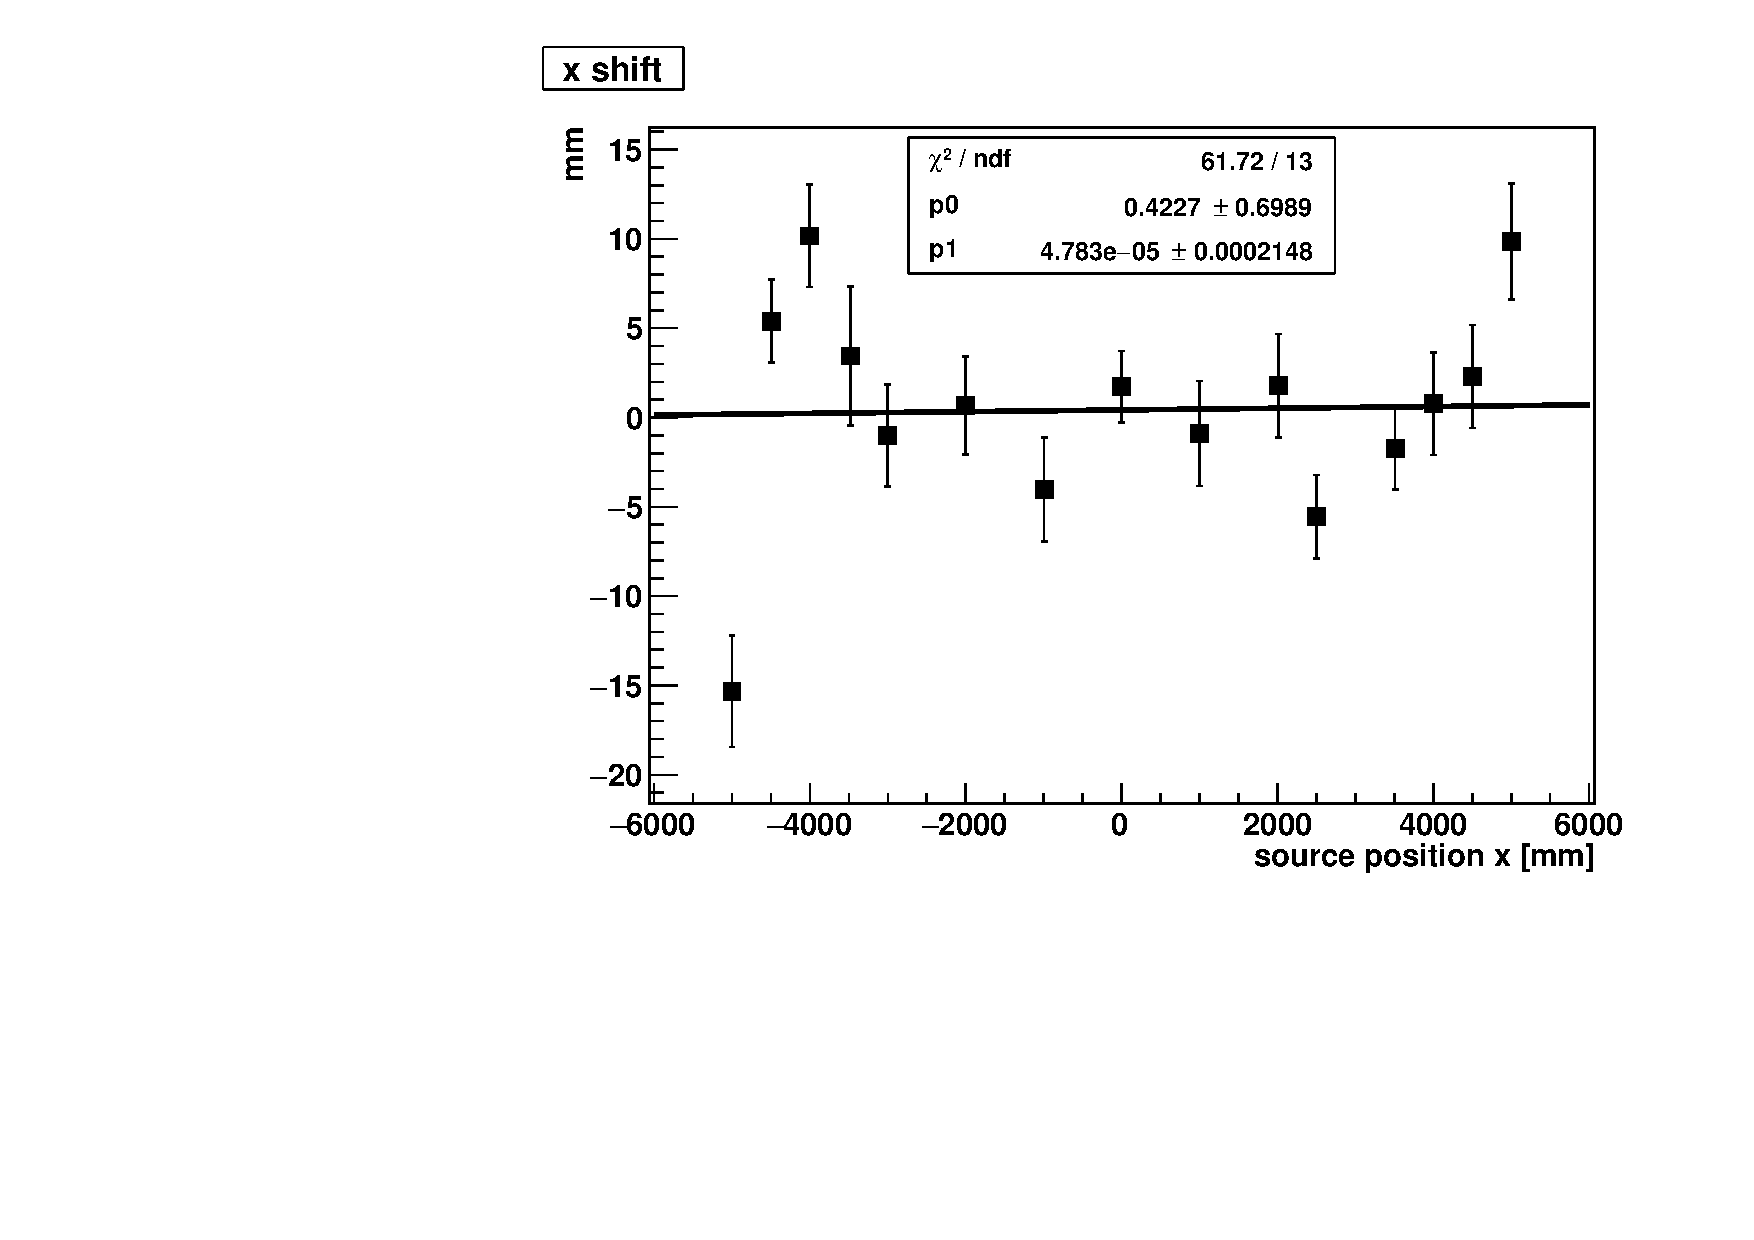
\includegraphics[width=8cm]{vertexScaleSysX.pdf}}
	\subfigure[$^{16}$N y-scan runs.]{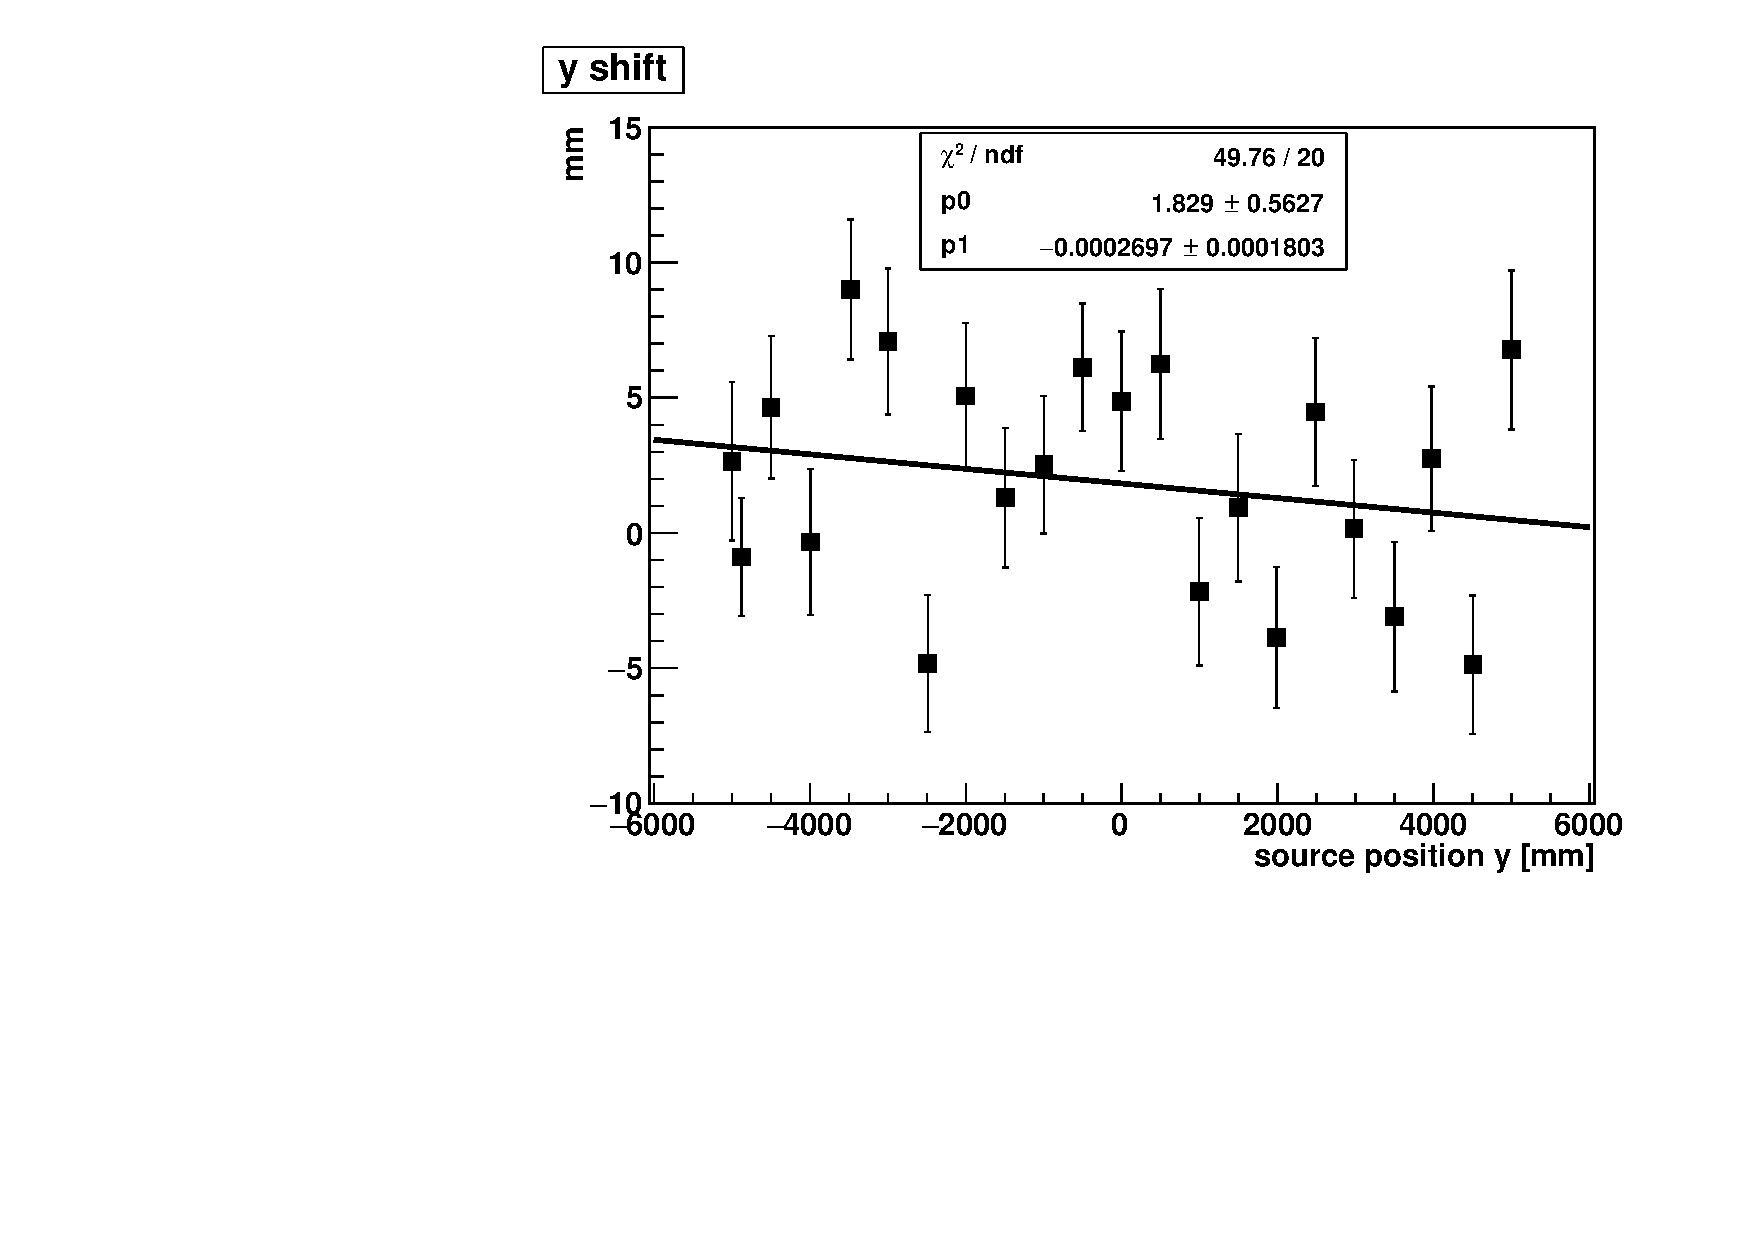
\includegraphics[width=8cm]{vertexScaleSysY.pdf}}
	\subfigure[$^{16}$N z-scan runs.]{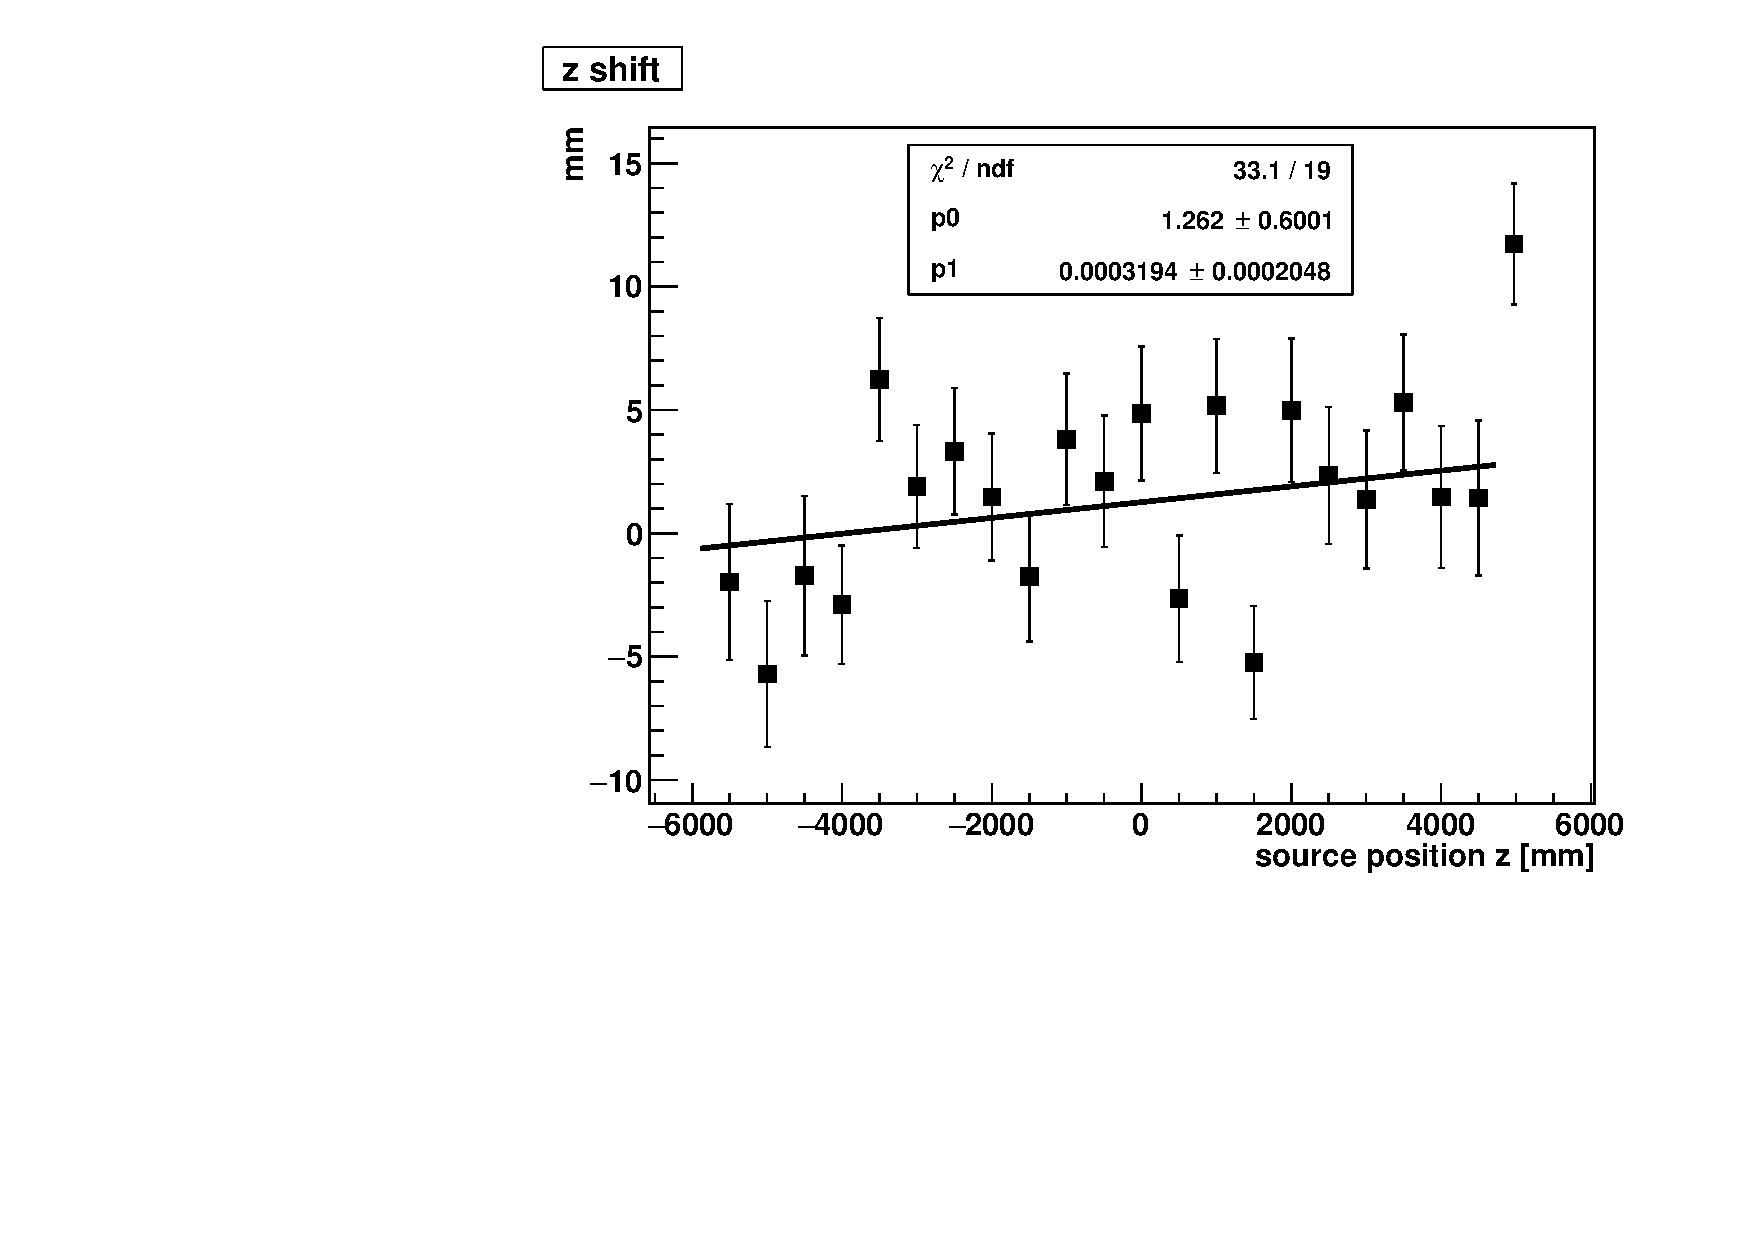
\includegraphics[width=8cm]{vertexScaleSysZ.pdf}}
	\caption{Vertex shifts along x, y, z axes and fitted with linear functions.\label{fig:vertexScale}}

\end{figure}

From the linear fits, the values of vertex shifts were obtained and listed in Table~\ref{tab:vertexScale}. Since the $\chi^2/\mathrm{ndf}$ values here were large, according to Refs.~\cite{pdg2020,waterunidoc}, inflated errors were calculated as $S\times$(slope errors), where the error scale factor $S=\sqrt{\chi^2/(\mathrm{ndf}-1)}$. The downward systematic was calculated as the slope minus the slope error as well as the inflated error. In contrast, the upward systematic was taken as the positive inflated error, as suggested by \cite{waterunidoc}. For the $z$ scan, the position at $(-185.037,247.24,4973.567)$ mm pulls the slope results to the positive, possibly due to the bias in simulation from the neck geometry effects. This point was not used in the linear fit.
%%%\footnote{John: {red}Here `ndf' means `number of degrees of freedom.' See ?? for background on this measure of goodness of fit.{red}}
\begin{table}[ht]
	\centering
	\caption{Vertex scales for the reconstructed positions on ($x, y, z$) axes.\label{tab:vertexScale}}
	\vspace{2mm}
	\begin{tabular*}{130mm}{c@{\extracolsep{\fill}}cccc}
		\toprule
		axis & fitted slope (\%)  & inflated error &systematic ($\delta^+/\delta^-$) (\%)\\
		\hline 
		$x$ scale &  0.005$\pm$0.021 & 0.048 & +0.07/-0.06\\	
		$y$ scale  & -0.027$\pm$0.018 & 0.030&  +0.02/-0.07\\
		$z$ scale & 0.032$\pm$0.020 & 0.027&  +0.08/-0.01\\
		\bottomrule
	\end{tabular*}
\end{table}

The vertex scale systematics were then transformed, e.g. $x'=(1+\delta_x/100)x$ with equivalent formulae for the $(y,z)$ axes.

The scale systematics also depend on the radius $r=\sqrt{x^2+y^2+z^2}$ \cite{waterunidoc}. By the usual logic for calculating error propagation, for an event position $(x,y,z)$, $\delta_r$ is calculated as\cite{waterunidoc}:
\begin{equation}
\delta_r =\sqrt{\sum_{i=1}^3(\frac{\partial r}{\partial x_i})^2 \; \delta^2_{x_i}}= \sqrt{\frac{x^2\delta_x^2+y^2\delta_y^2+z^2\delta_z^2}{r^2}}\; .
\end{equation}
Using the $\delta^+$ and $\delta^-$ for $(x,y,z)$ scales in Table~\ref{tab:vertexScale}, the $\delta_r^+$ and $\delta_r^-$ are calculated, respectively. Then the two-sided bounds for the confidence interval of reconstructed radius $r$ are calculated by as $r^+=(1+\delta^+_r/100) \; r$ and $r^-=(1+\delta^-_r/100) \; r$.

%Uncertainties from the source manipulator positions are assumed to be 50~mm.

\subsection{Direction Reconstruction Evaluation}

\subsubsection{Direction Resolution}

For reconstructed $^{16}$N calibration events, on the assumption that a $\gamma$ photon emitted by the source interacted with an electron at the reconstructed position, the ``true'' direction of an event is defined as the direction pointing from the source manipulator position to the reconstructed position,
\begin{equation}
\vec{u}_{\mathrm{true}} = \frac{\vec{X}_{\mathrm{fit}}-\vec{X}_{\mathrm{src}}}{|\vec{X}_{\mathrm{fit}}-\vec{X}_\mathrm{src}|} \; .
\end{equation}
Now define $\theta$ as the angular difference between the ``true'' and the reconstructed event orientations, viz. $\cos\theta= \vec{u}_{\mathrm{true}} \cdot \vec{u}_{\mathrm{fit}}$.

The distribution of $\cos\theta$ was fitted with the direction resolution function (Eqn.~\ref{eq:directResol}) mentioned in Sect.~\ref{sect:directResol}. Before the fitting, a few cuts relating to the position and energy reconstructions were applied to the data or simulation results. As mentioned in Chapter 4, the direction reconstruction relies on the position. Therefore, the $posFoM$ cut ($scaleLogL>10$) was applied before evaluating the direction reconstruction. Other cuts were suggested by the SNO+ collaboration to remove instrumental backgrounds, and poor reconstructions for events close to the source container or far away from the source. To remove instrumental backgrounds, the cuts
\begin{itemize}
\item $E_{fit} > 3.5$ MeV\;,
\item ITR$>0.55$\;,
\item $-0.12<\beta_{14}<0.95$\;,
\end{itemize}
were used. To remove poorly reconstructed events which were close to the source container due to its shadow effect, and also the events far away from the source, a distance cut, $1000<|\vec{X}_{fit}-\vec{X}_{src}|<2300$ mm, was applied. For the internal scans, a radius cut $R'<5850$ mm was also applied. This radial cut was not applied on the external and neck scans \cite{waterunidoc}.

Fig.~\ref{angularResolMPW} shows the fitted results of the angular distributions over a fit range (in $\cos \theta_e$) of [0.3,1], after the cuts mentioned, and the resolution parameters are shown in Table~\ref{tab:angularResolValuesUpdated}. Direction resolution for the MC is better than for the data, due to the idealized (simpler) configuration modelled in the simulations. The reconstruction performances of the \texttt{MPW fitter} and the \texttt{RAT water fitter} are similar, while for both the detector data and MC, $\beta_M$ values yielded by \texttt{MPW} are about 10\% higher than those from \texttt{RAT}. In short, direction resolution of the \texttt{MPW} is slightly better than that of the \texttt{RAT}.

\begin{figure}
	\centering
	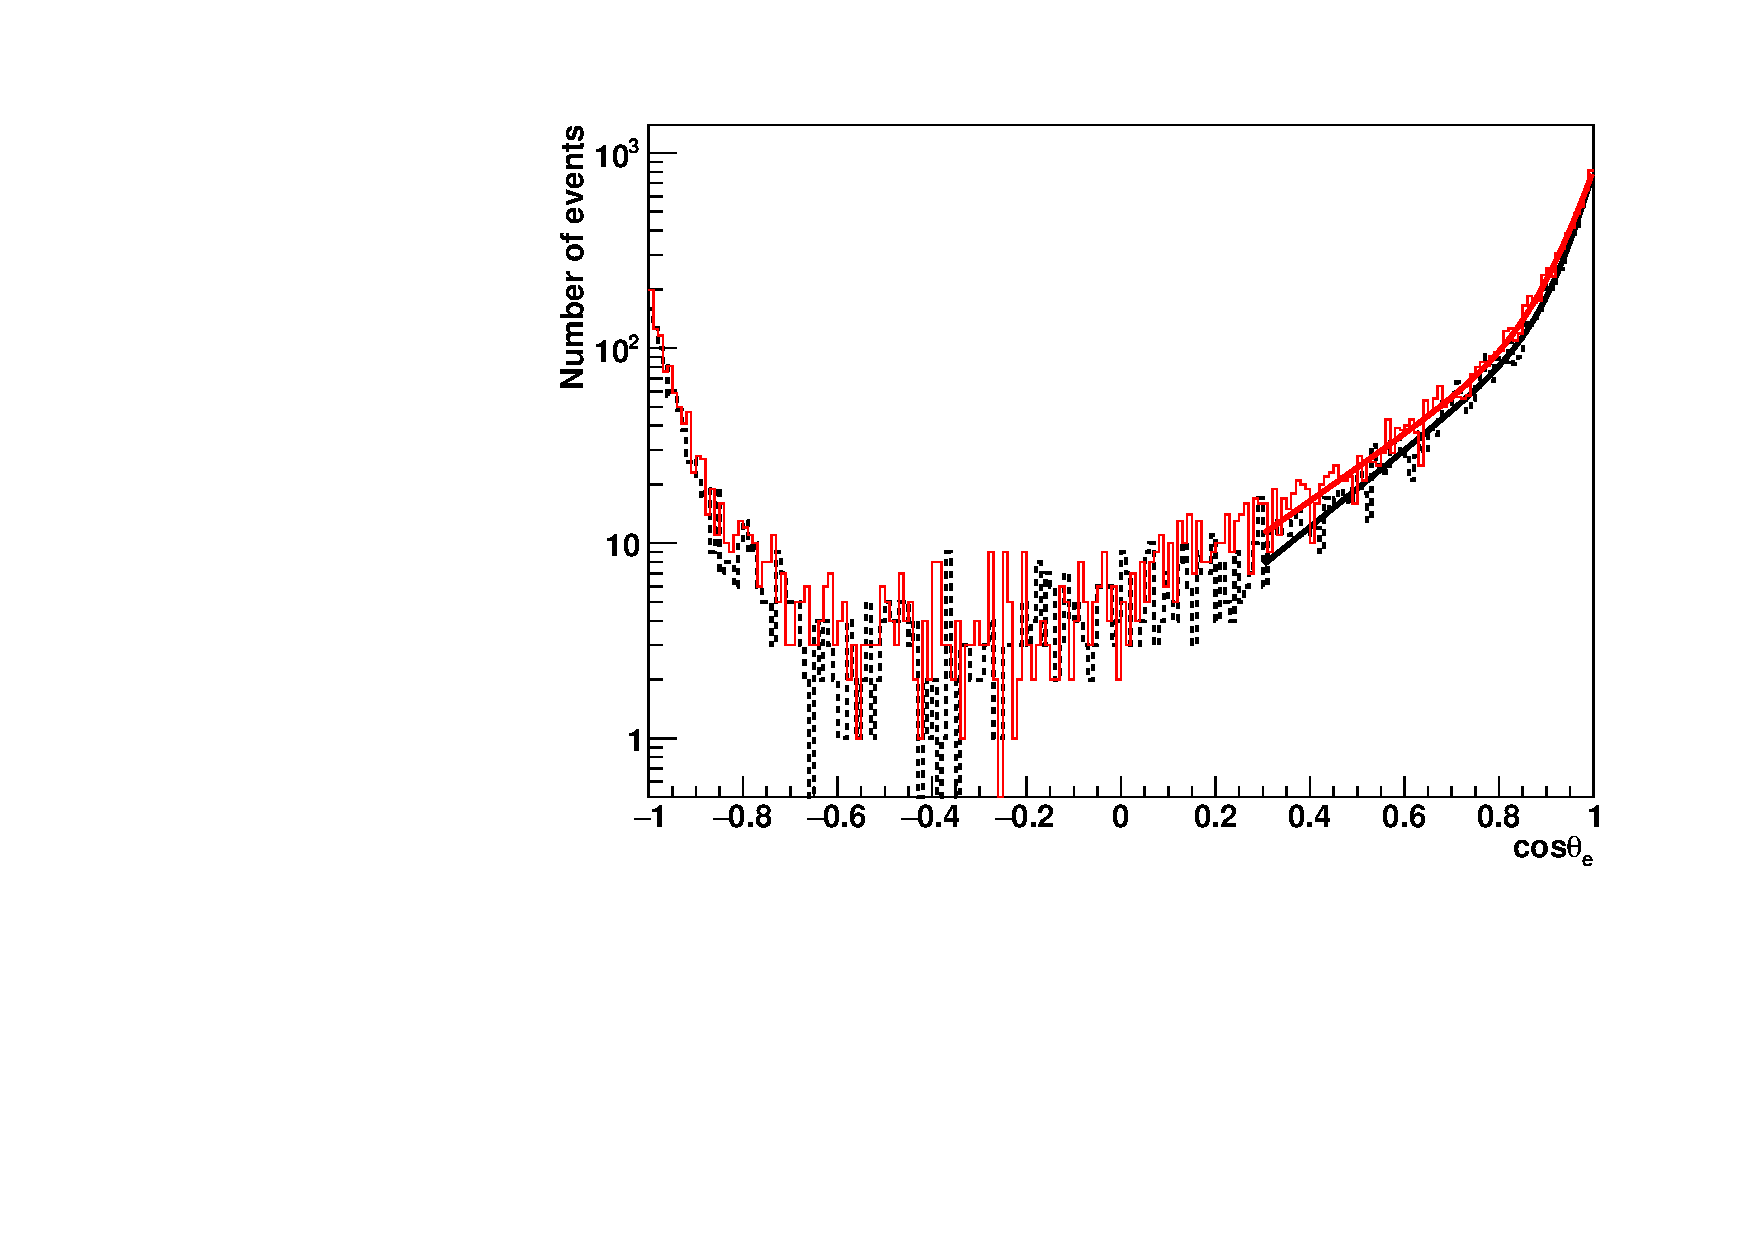
\includegraphics[width=10cm]{16NangularResol.pdf}
	\caption[Distributions of the angular error in direction reconstruction, from the data and from MC.]{Distributions of the angular error in direction reconstruction, from the data (red solid line) and MC (black dashed line); both are reconstructed by the \texttt{MPW fitter}. These distributions are fitted with the angular resolution functions over the range [0.3,1].\label{angularResolMPW}}

\end{figure}

\begin{table}[ht]
	\caption[Direction resolution of the \texttt{MPW} and \texttt{RAT} fitters.]{Direction resolution of the \texttt{MPW} and \texttt{RAT} fitters, when applied to $^{16}$N calibration data and when applied to MC simulations of the calibration process.\label{tab:angularResolValuesUpdated}}
	\begin{tabular}{cccccccc}%{|p{2.2cm}|p{1.8cm}|p{2cm}|p{2cm}|p{1.8cm}|p{1.1cm}|p{1.1cm}|p{1.1cm}| }
		\toprule
	107055& $\beta_M$ &  $\beta_S$ & $\alpha_M$ & $\chi^2$/ndf & $\cos\theta_{0.5}$ & $\cos\theta_{0.8}$& $\cos\theta_{0.9}$\\
	\hline
	\texttt{MPW} data & 4.15$\pm$0.18 & 19.08$\pm$0.94 & 0.58$\pm$0.02 & 77.1/66 & 0.964 & 0.744 & 0.410 \\
	\texttt{MPW} MC & 4.42$\pm$0.19 & 20.41$\pm$1.01 & 0.56$\pm$0.02 & 83.8/66 & 0.974 & 0.768 & 0.454	 \\	
\hline
	\texttt{RAT} data & 3.76$\pm$0.18 & 17.90$\pm$0.82 & 0.55$\pm$0.02 & 70.5/66 & 0.974 & 0.731 & 0.364 \\
	\texttt{RAT} MC & 4.02$\pm$0.18 & 20.89$\pm$0.92 & 0.54$\pm$0.03 & 94.9/66 & 0.979 & 0.753 & 0.409	\\
		\bottomrule
	\end{tabular}
\end{table}

\subsubsection{Direction Systematics}

For all the internal $^{16}$N scans, the cuts mentioned in the previous section were applied on both the data and simulations. In a manner similar to that when evaluating the positional uncertainties, the angular resolution function was first fitted with three free parameters: $\alpha_M$, $\beta_S$, and $\beta_M$. To simplify the calculation in propagating systematics, an average value of the fitted $\alpha_M$ was calculated from all the internal scans (except the three neck scans), namely $\alpha_M =  0.613$ for data and $\alpha_M = 0.585$ for MC. With these fixed values for $\alpha_M$, both the data and the MC were refitted to extract $\beta_S$ and $\beta_M$ only. The default fit range (in $\cos \theta_e$) was [0.3,1], however for some scans when the source was close to the AV the event count, after the cuts, was too low. For those situations, to ensure more than 5000 events were fitted, the fit range was enlarged by moving a 0.1 step leftward, until the negative-most value reached -0.5: $[0.3-0.1 \cdot step, 1]$.

Fig.~\ref{angularResolScan} shows the results for the fitted $\beta_M$ and $\beta_S$ values for the internal $^{16}$N $(x,y,z)$-axis scans. For {\em most} scans, the MC results are better than the data. The three $Z$ scans in the neck provided the least satisfactory direction resolutions, due to the asymmetry of the detector geometry.

\begin{figure}
	\centering
	\subfigure[$^{16}$N $x$-scan runs.]{\label{angular:xscan}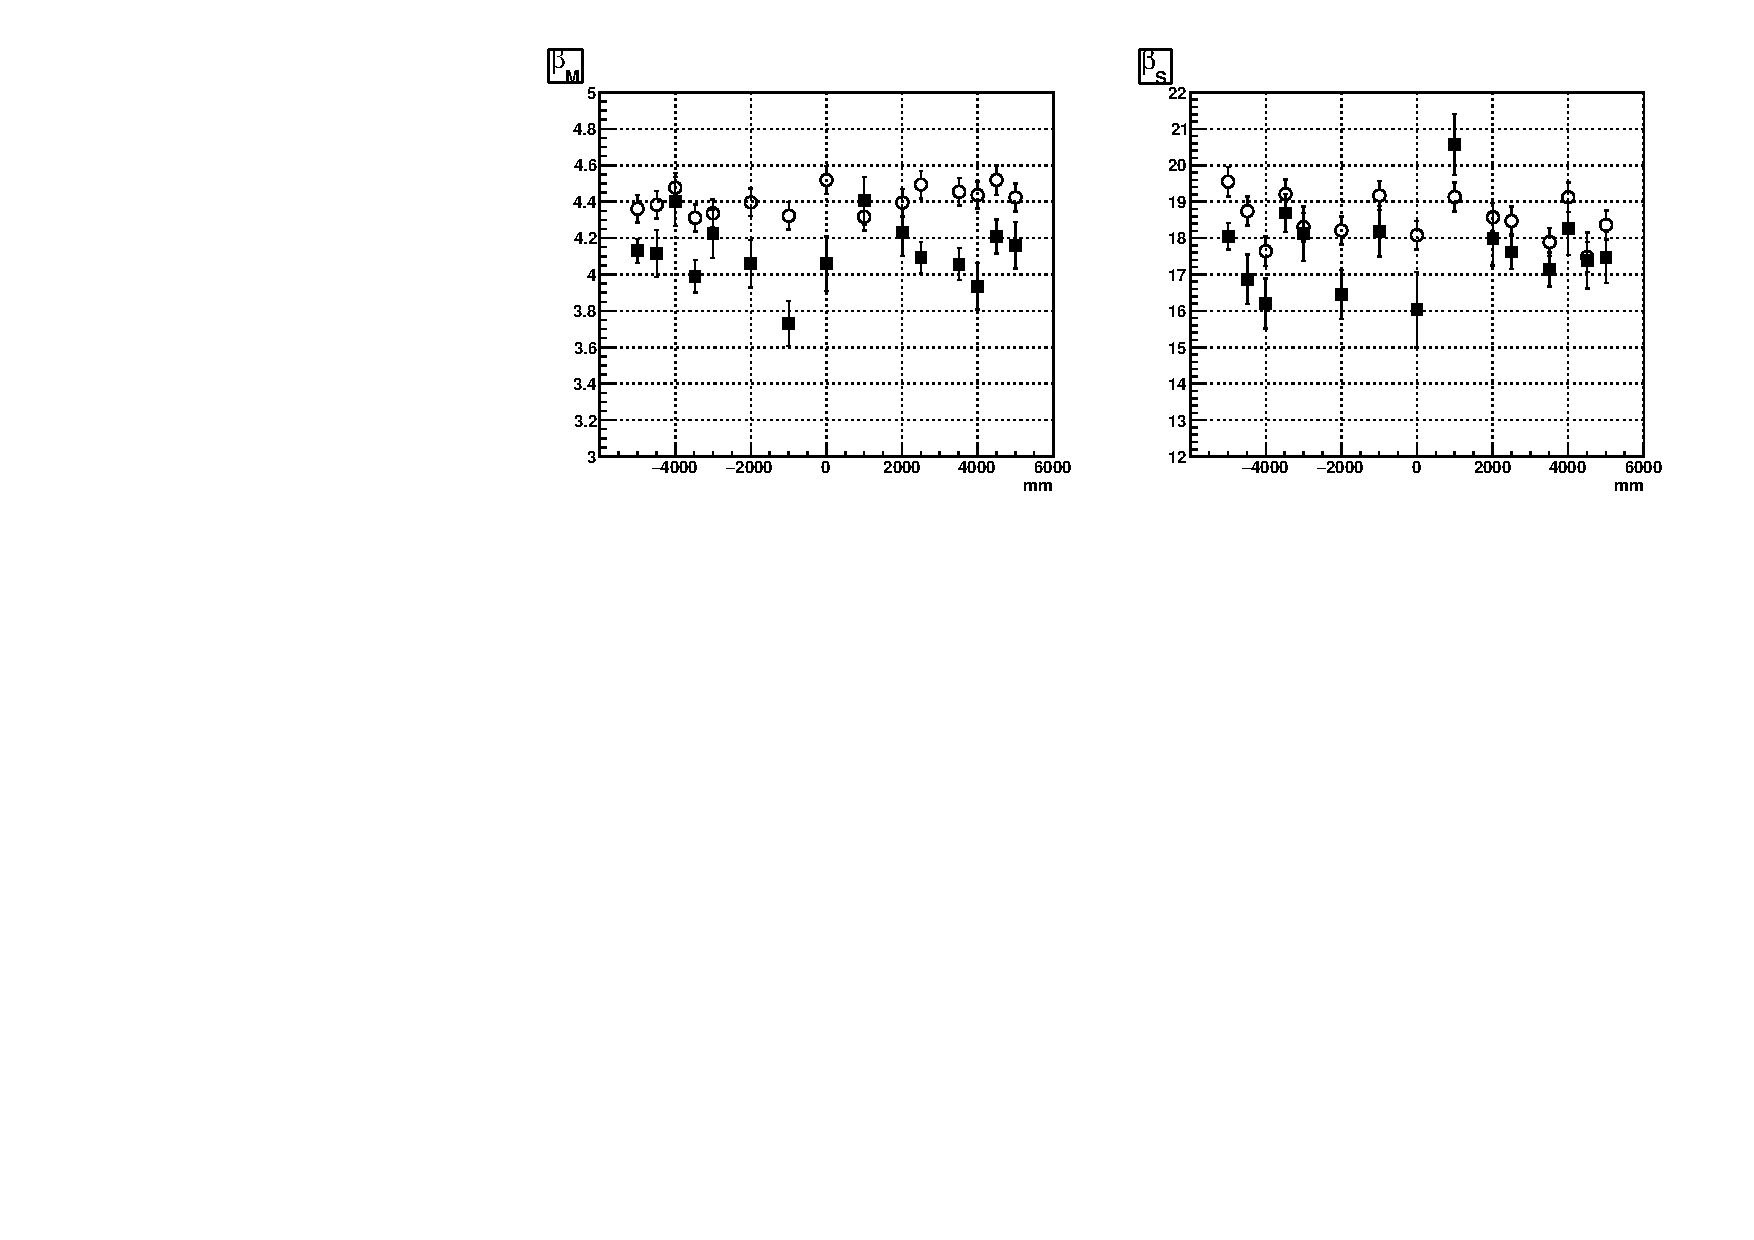
\includegraphics[width=12cm]{16NangularScan_x.pdf}}
	\subfigure[$^{16}$N $y$-scan runs.]{\label{angular:yscan}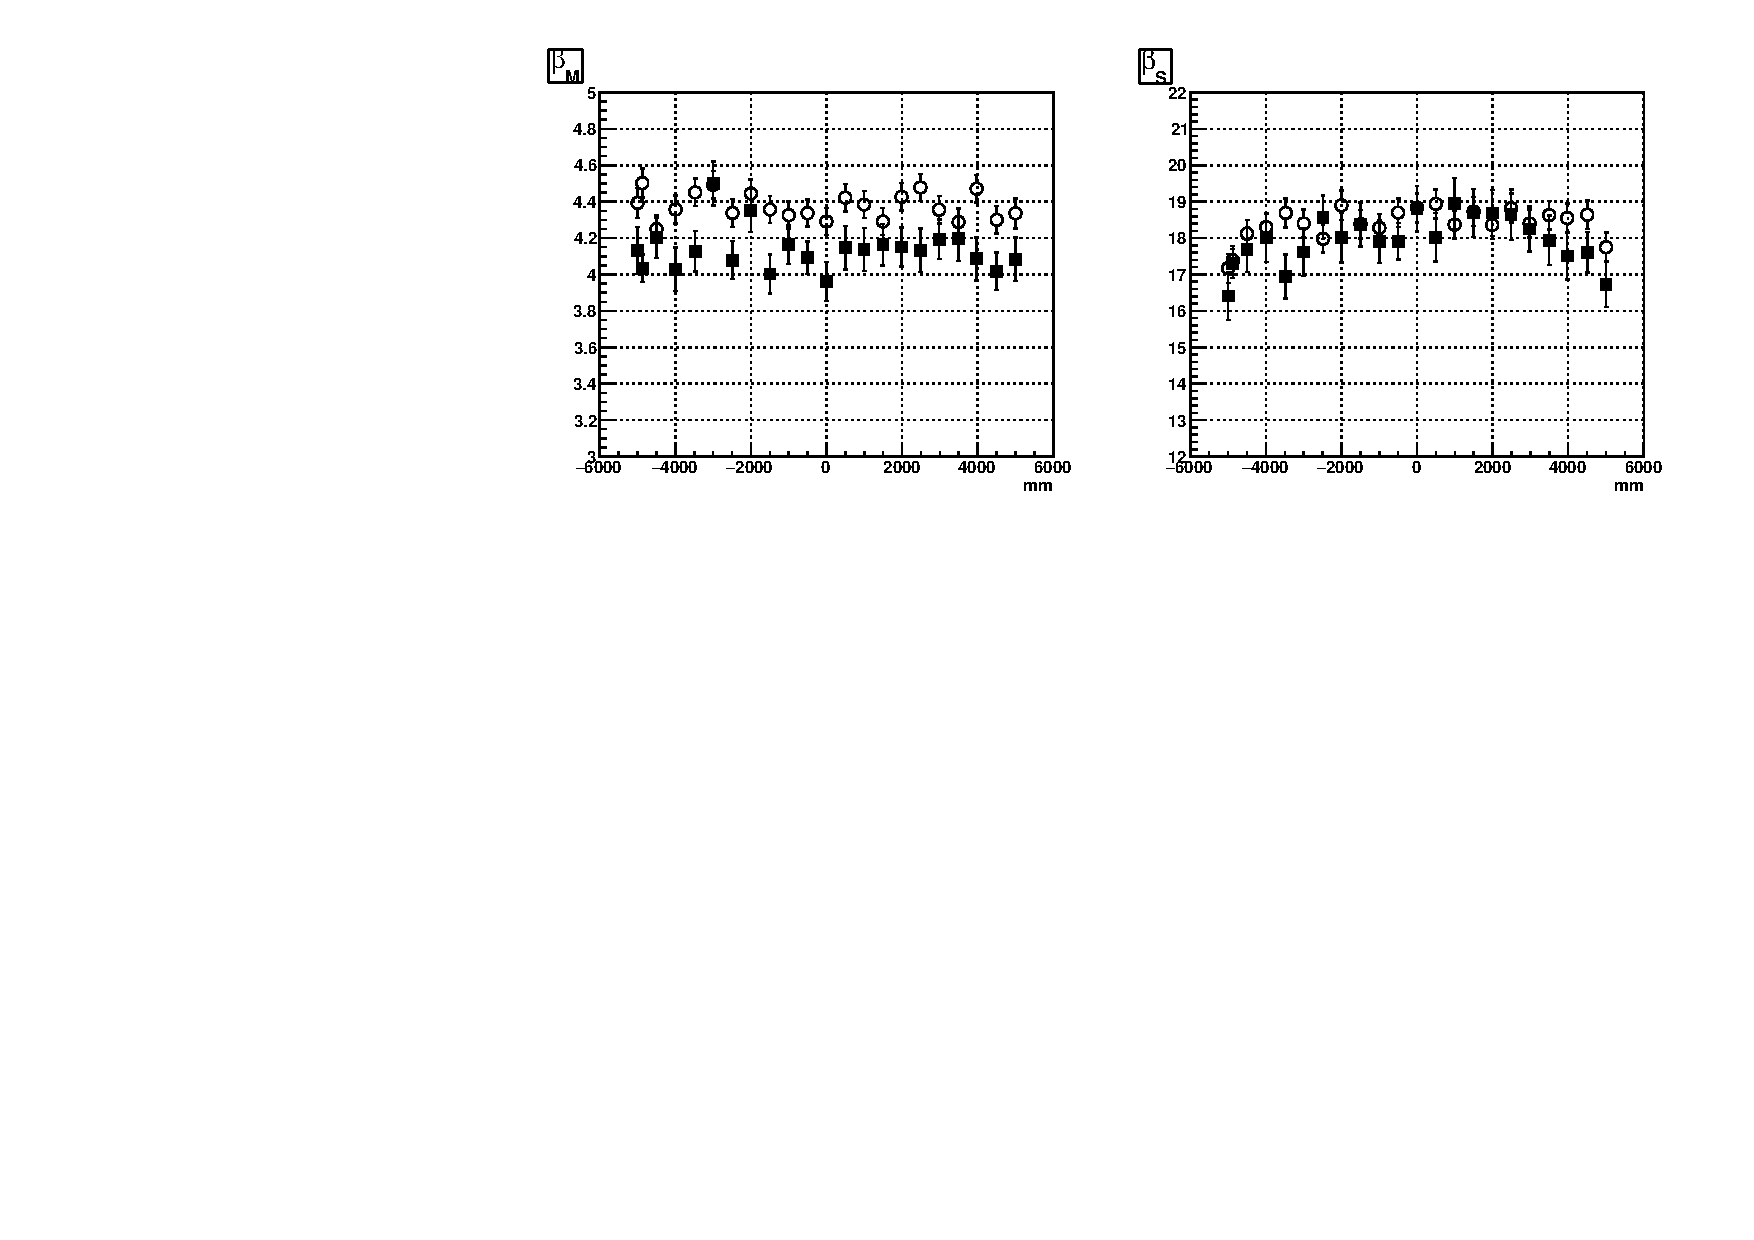
\includegraphics[width=12cm]{16NangularScan_y.pdf}}
	\subfigure[$^{16}$N $z$-scan runs.]{\label{angular:zscan}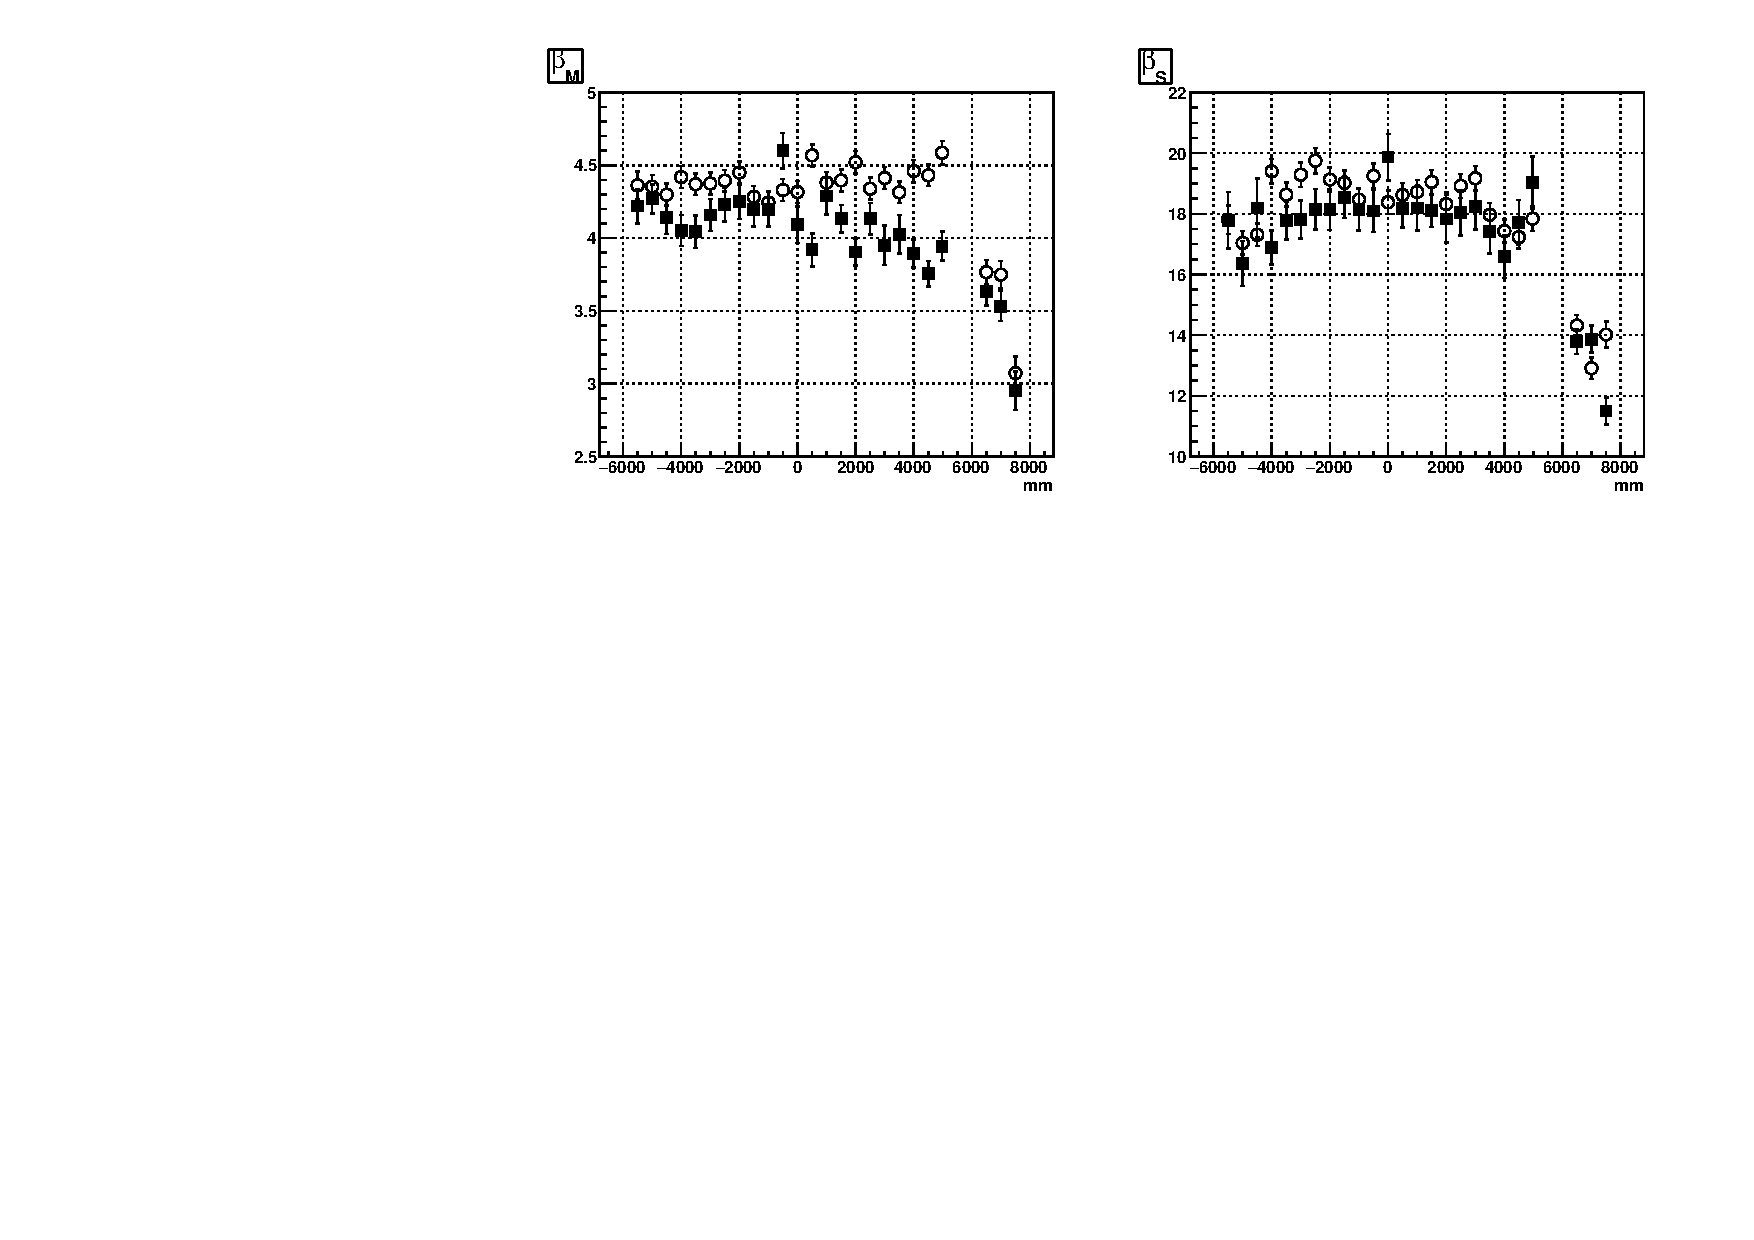
\includegraphics[width=12cm]{16NangularScan_z.pdf}}
	\caption[Fitted direction resolution parameters $\beta_M$, $\beta_S$ for the source scans.]{Fitted direction resolution parameters $\beta_M$, $\beta_S$ for the source scans on ($x, y, z$)-axes respectively. Solid squares, MC; Open circles, data.\label{angularResolScan}}
\end{figure}

The relative difference between data and MC of a fitted resolution quantity $q\pm \delta_q$ is defined as
\begin{equation}
(\Delta q)_{rel} = \frac{q_{data}-q_{MC}}{q_{MC}}\times 100\%\;,
\end{equation}
and the error of the relative difference is defined as 
\begin{equation}
\delta_{(\Delta q)_{rel}} = \sqrt{(\frac{\delta_{q_{data}}}{q_{data}})^2+(\frac{\delta_{q_{MC}}}{q_{MC}})^2}\times 100\% \; .
\end{equation}\label{eq:erors_relativeBiases}

Fig.~\ref{relative_biasesVsPositions} shows the relative differences for the internal $(x, y, z)$ scans (excluding the neck scans). Based on those scans (i.e. the internal scans barring those with the source in the neck, leaving 77 runs in total) the means and standard deviations of the relative differences are $\Delta(\beta_M)_{rel}=(-6.09\pm4.01)\%$ and $\Delta(\beta_S)_{rel}=(-3.09\pm4.39)\%$.

To be conservative, taking the largest and smallest values of the $\Delta(\beta_M)_{rel}$ and $\Delta(\beta_S)_{rel}$, the negative and positive values of the direction systematic ($\delta_\theta$) are obtained as $\delta_\theta=+0.013/-0.101$.

\begin{figure}[!htb]
	\centering
	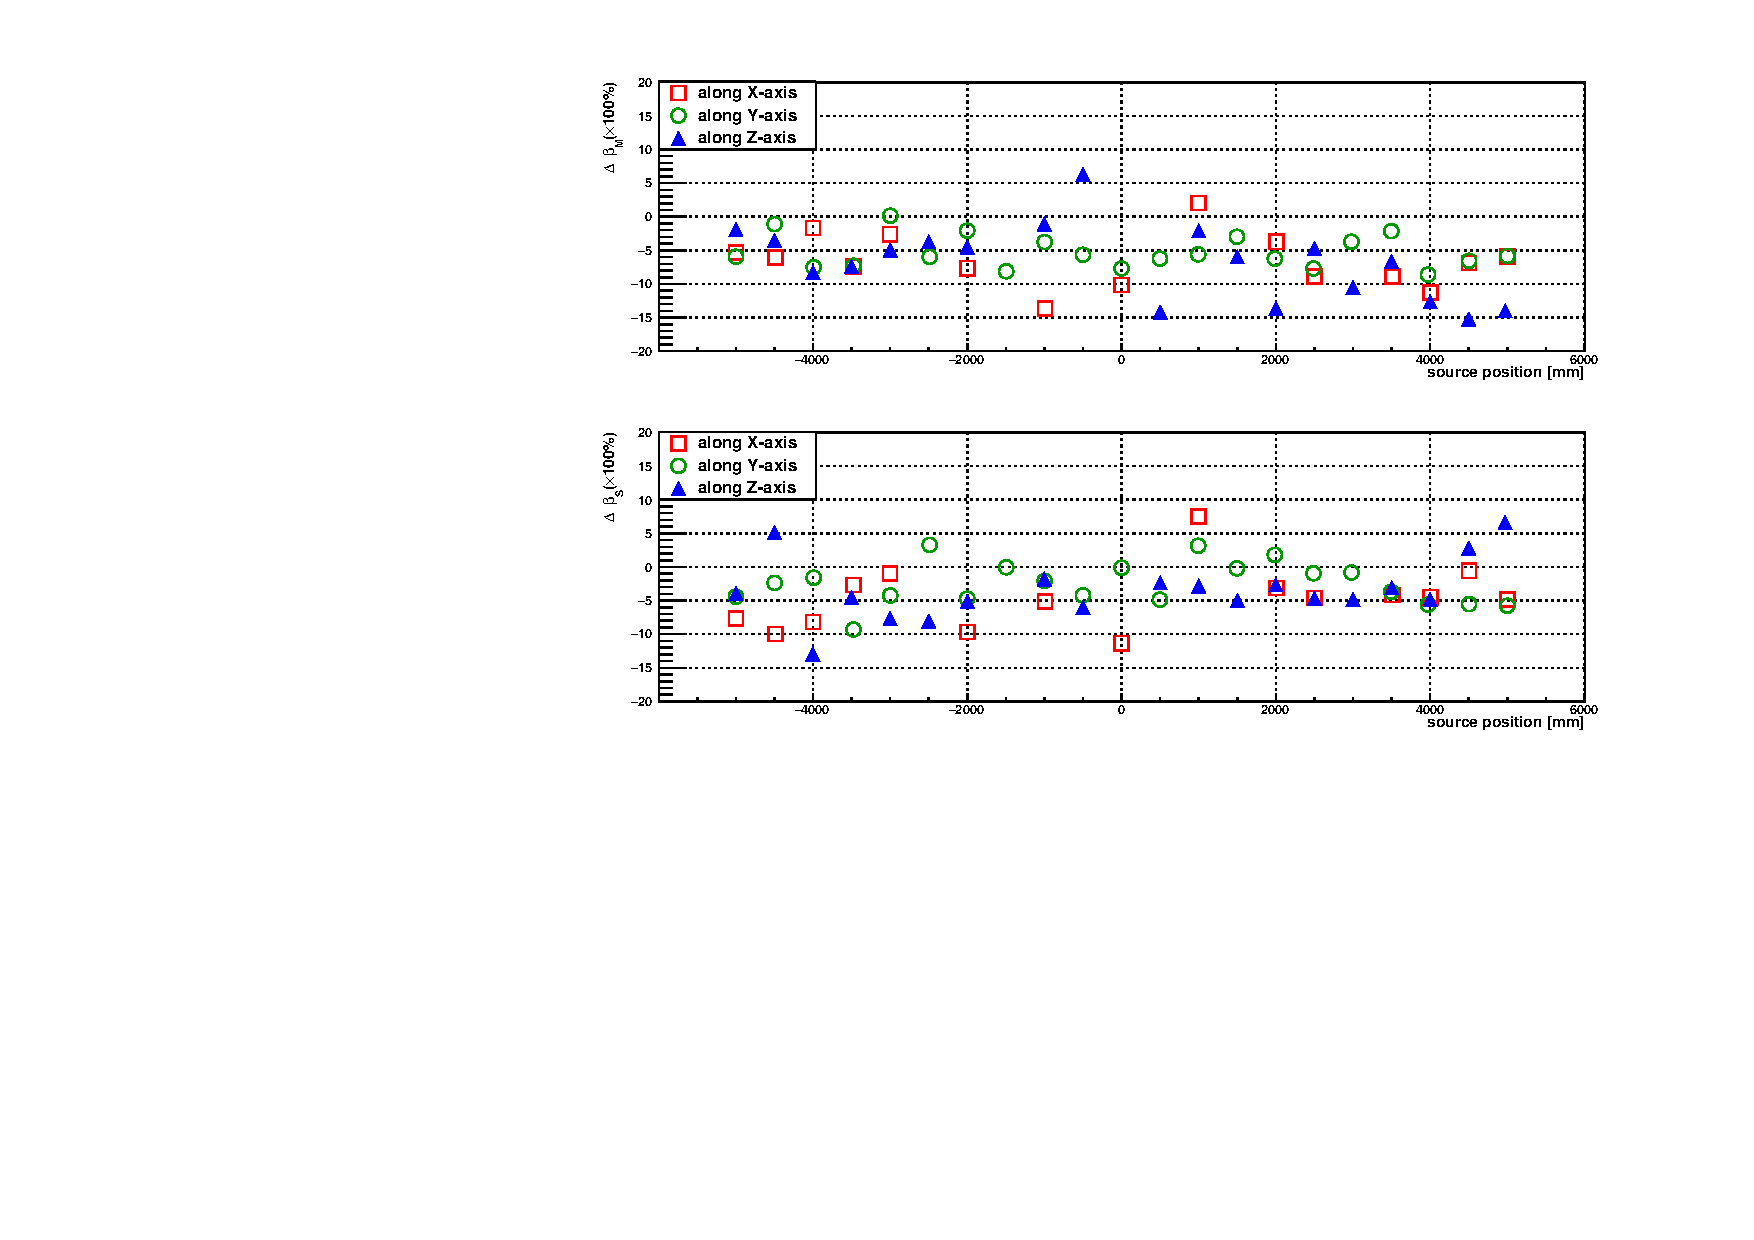
\includegraphics[width=16cm]{angularResol_scanXYZ.pdf}
	\caption[Relative differences of $\beta_M$ and $\beta_S$ as a function of the $^{16}$N source position.]{Relative differences of $\beta_M$ and $\beta_S$ as a function of the $^{16}$N source position. For simplicity, the corner scans are not shown in this figure. The red squares represent the results from the $x$-scan runs; green circles represent the $y$-scan runs and the blue triangles represent the $z$-scan runs. \label{relative_biasesVsPositions}}
\end{figure}

To propagate the uncertainties in $\beta_M$ and $\beta_S$ to the direction resolution, a first-order approximation function was derived by the SNO collaboration\cite{drouin2012three}:
\begin{equation}\label{remapTheta}
\cos\theta'=1+(\cos\theta-1)(1+\delta_{\theta}) \, .
\end{equation}

This angular remapping function was used to smear the angular distributions for systematic studies. In the next chapter, it will be applied on the angular distribution of solar neutrino data. 

\subsection{$\beta_{14}$ and its Systematic}

Since $\beta_{14}$ itself is used as the high-level cut, only the cuts $\mathrm{ITR}>0.55$ and $\mathrm{NHits}>5$ were applied on the data and MC to extract the $\beta_{14}$ distributions. Fig.~\ref{fig:N16beta14} shows the $\beta_{14}$ distributions of the central run 107055 data and MC, reconstructed by the \texttt{MPW fitter} and the official \texttt{RAT} fitter respectively. The $\beta_{14}$ is calculated based on the reconstructed position, time, and direction of an event, and the $\beta_{14}$ distributions from the \texttt{MPW} and \texttt{RAT} fitter results are consistent. However, both fitters show a discrepancy between the data and the MC, a discrepancy that may be caused by inaccurate modeling of the Cherenkov process in the Geant4 simulation\cite{dunmore2004separation,beta14discrepancy}. Fig.~\ref{fig:N16beta14MPW} compares the $\beta_{14}$ values from the data and the MC of run 107055. Both of the distributions are the MPW processed results and are fitted with Gaussian distributions over the range $-0.5 \le \beta_{14} \le 1.5$. The data shows a slightly smaller Gaussian mean value, $\mu_{data}=0.4157$, compared to $\mu_{MC}=0.4388$.

\begin{figure}[htbp]
	\centering
	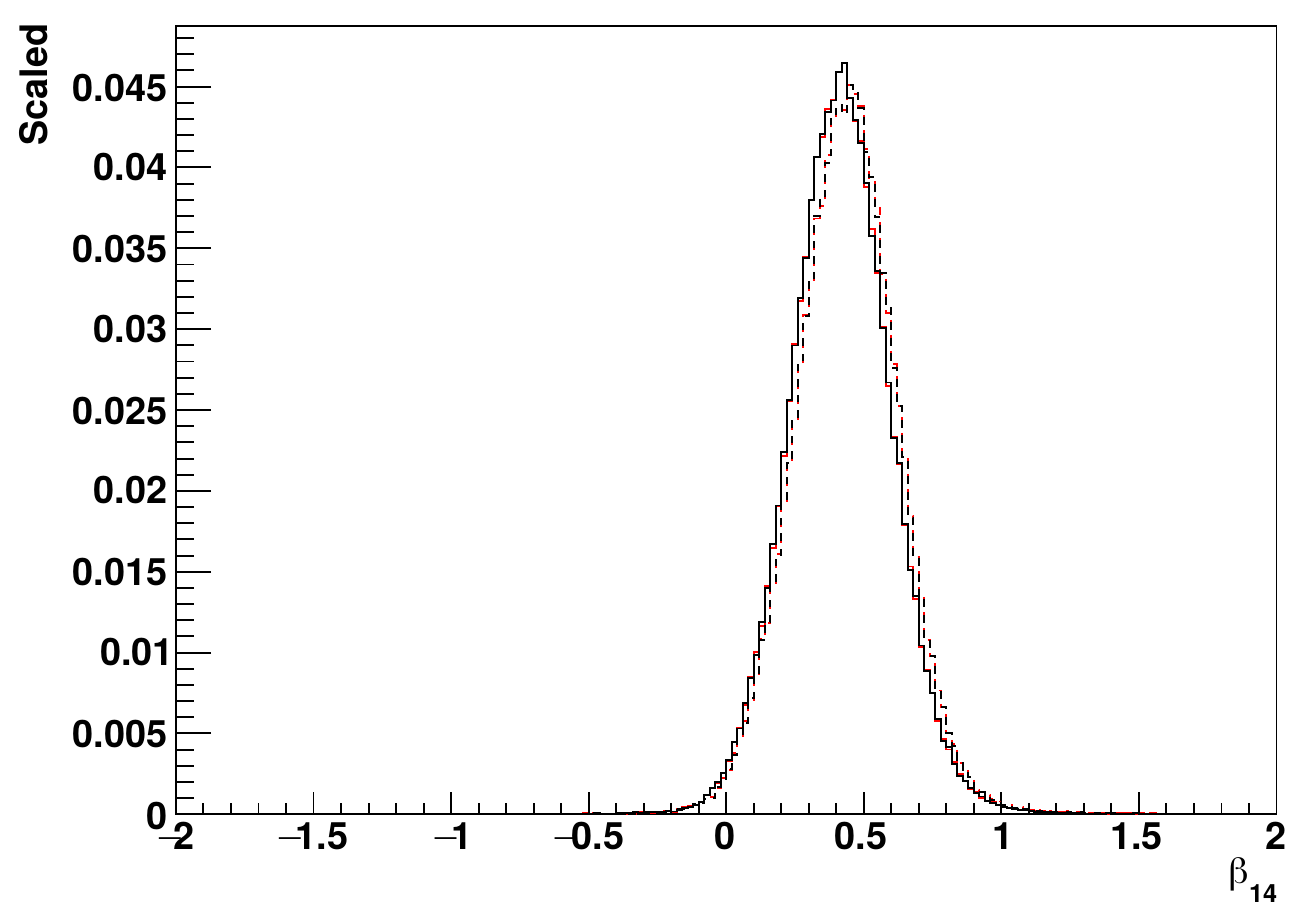
\includegraphics[width=8cm]{N16_beta14_107055.png}
	\caption[Distributions of $\beta_{14}$ for the $^{16}$N central run 107055.]{Distributions of $\beta_{14}$ for the $^{16}$N central run 107055. Dashed lines for the MC and solid lines for data; red for the \texttt{MPW fitter} processed results and black for the \texttt{RAT} results. \label{fig:N16beta14}}
\end{figure}

\begin{figure}[htbp]
	\centering
	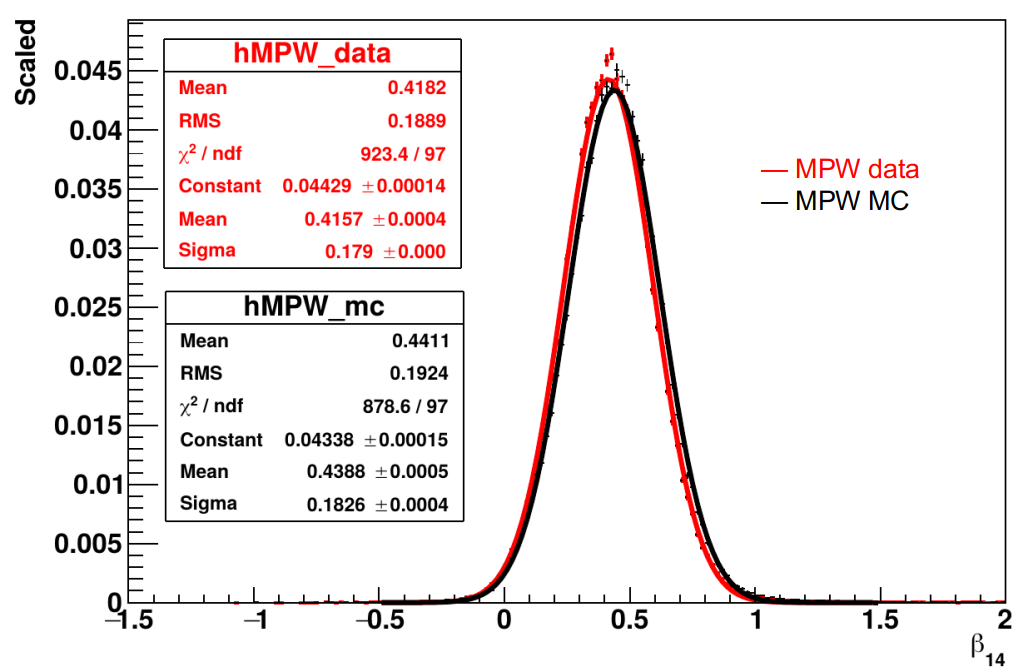
\includegraphics[width=8cm]{N16FitMPW_beta14_107055.png}
	\caption{A comparison of the $\beta_{14}$ for the data and the MC in run 107055. \label{fig:N16beta14MPW}}
\end{figure}

Fig.~\ref{beta14_XYZscans} shows the effects on $\beta_{14}$ when source position is moved along the ($x, y, z$) axes. $\Delta \beta_{14}\equiv\mu_{data}-\mu_{MC}$ was calculated for each of the 80 internal runs (i.e. including neck runs), and the mean and standard deviation of these $\Delta \beta_{14}$ values were taken as the shift in $\beta_{14}$: $-0.026\pm0.010$. Following the suggestion in Ref.~\cite{waterunidoc}, an asymmetric uncertainty was taken: the upward shift was taken as $+0.010$ while the downward shift was taken as $-0.026-0.01=-0.036$. Thus the shifts $+0.010/-0.036$ were taken as the $\beta_{14}$ systematics, and will be applied to the solar neutrino analysis in the next chapter. 

\begin{figure}[htbp]
	\centering
	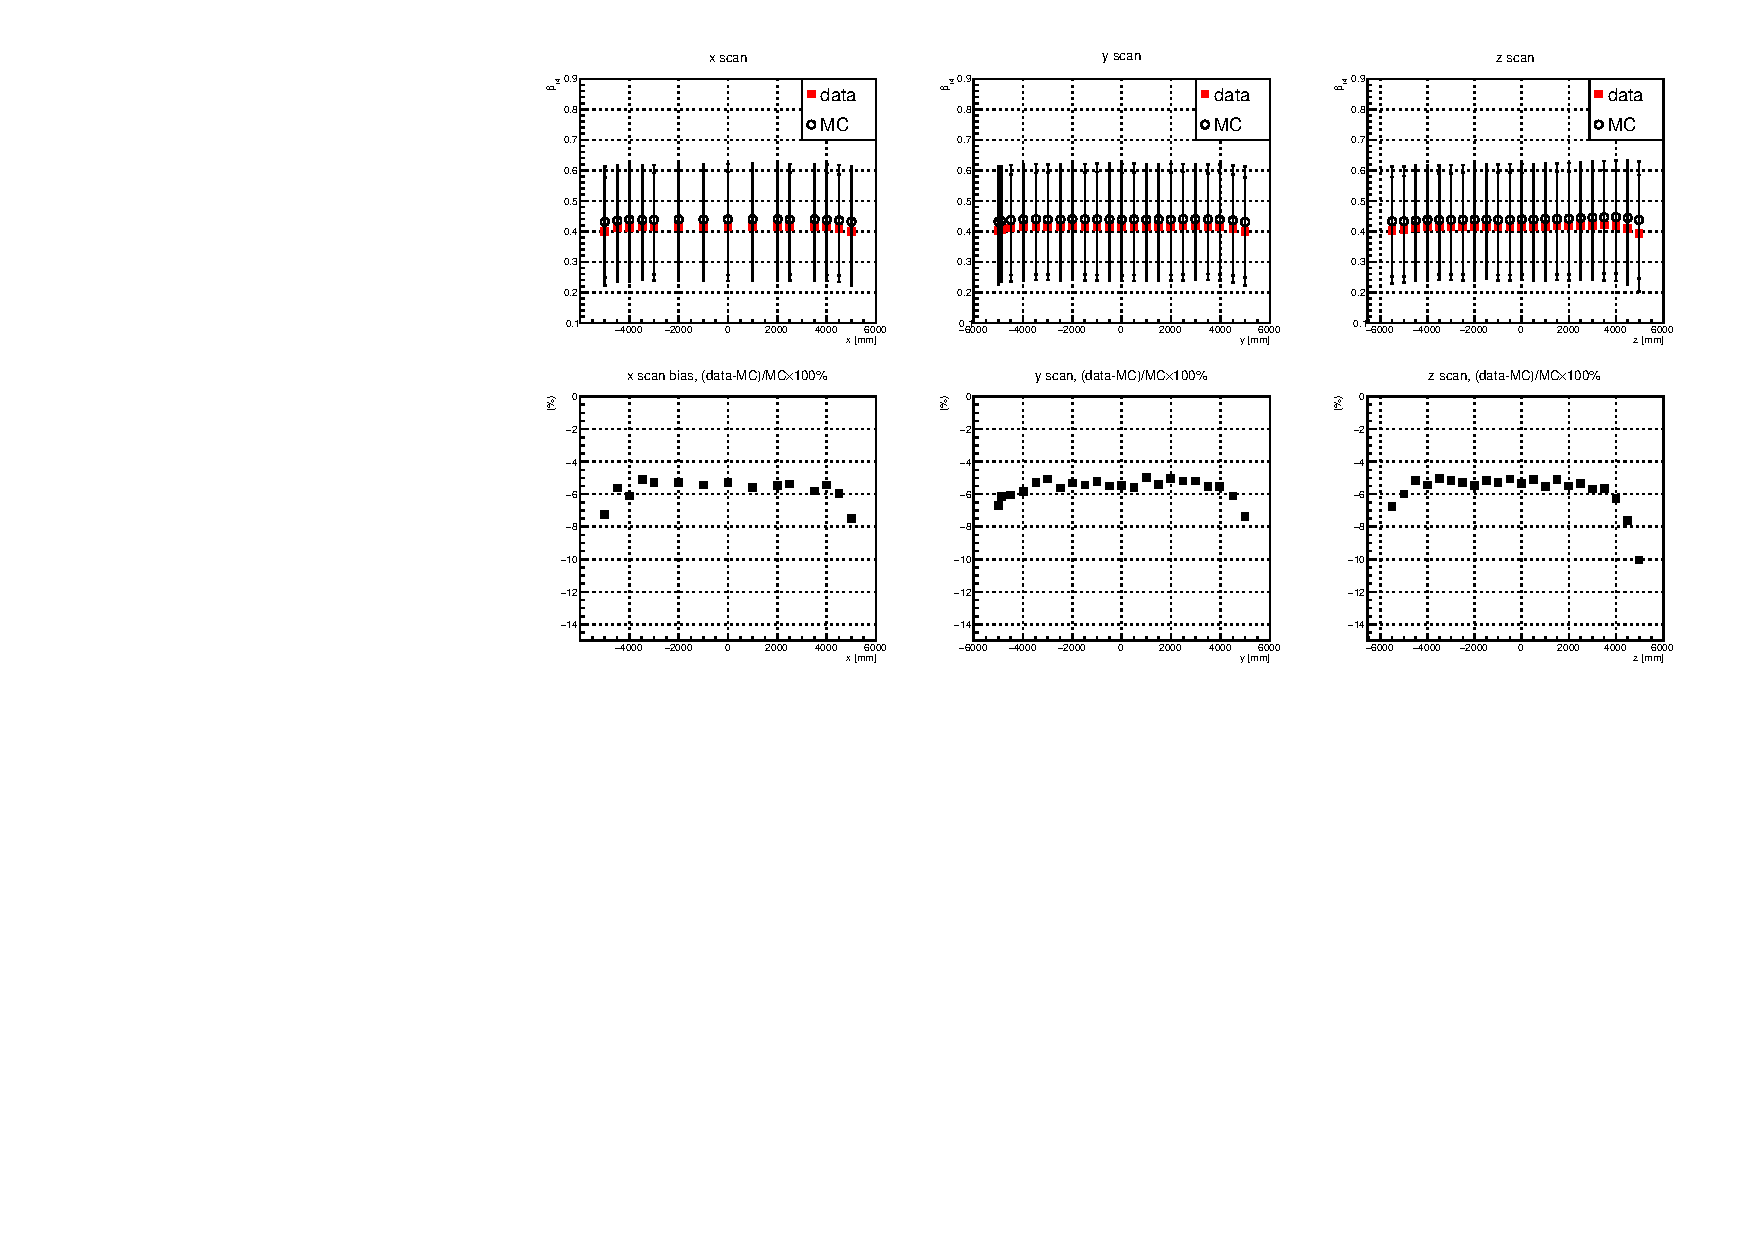
\includegraphics[width=16cm]{beta14_xyzScans.pdf}
	\caption{$\beta_{14}$ systematic along $(x, y, z$) scans.	\label{beta14_XYZscans}}
\end{figure}
%Discussions for the external scan runs.
%For external scans, the radial cuts were not applied. 

%\begin{figure}[!htb]
%	\centering
%	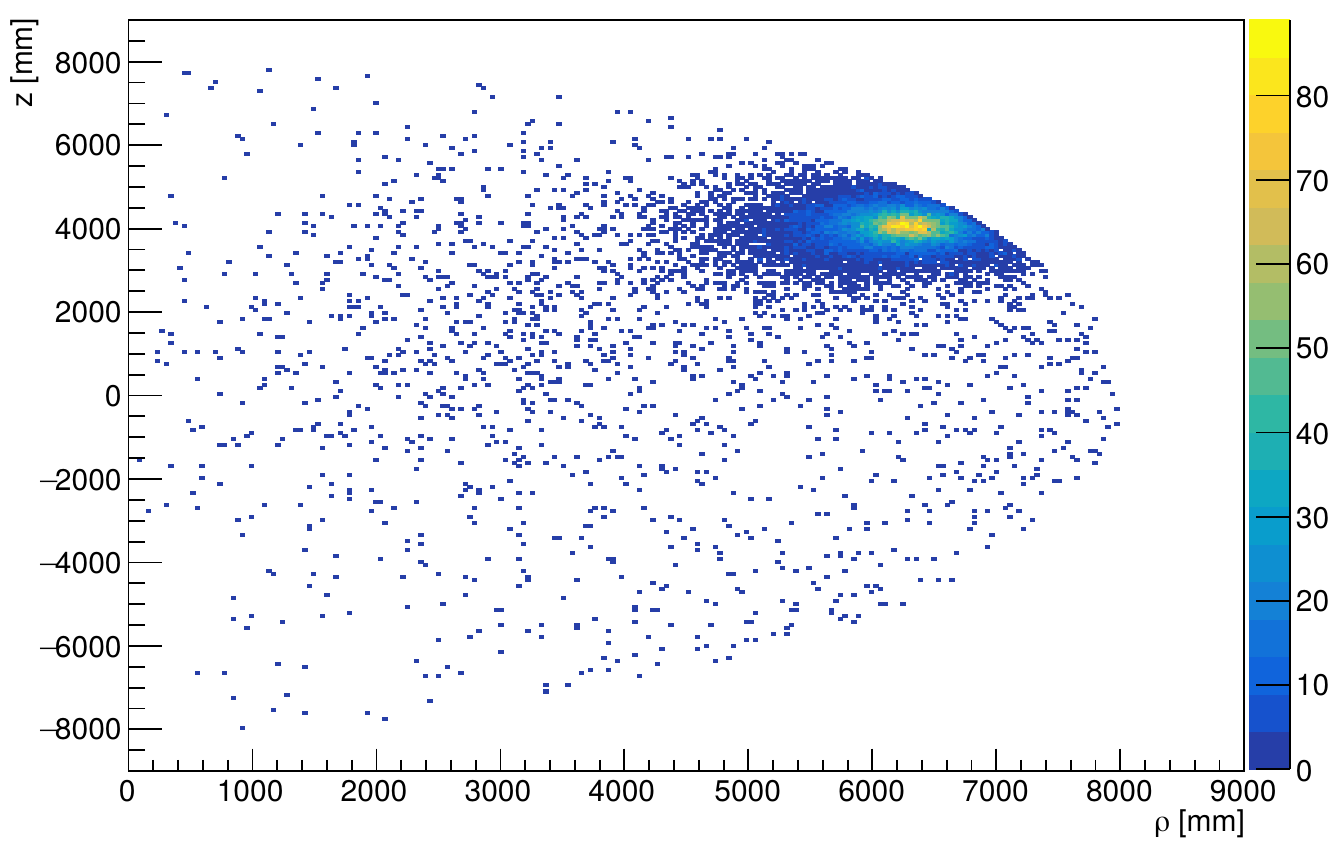
\includegraphics[width=8cm]{N16_external_111230_rhoZ.png}
%	\caption{$^{16}$N external run-111230 with a nominal position at [-5861,-2524,4001] mm; MPW results.}
%	\label{16Nexternal}
%\end{figure}

\subsection{Energy Reconstruction Evaluation}

\subsubsection{Energy Figure of Merits}\label{sect:energy_fomTest}

Three energy FoM quantities, namely $G_{test}$, $U_{test}$ and $Z_{factor}$, were introduced in Sect.~\ref{sect:energy_fom}. Here I used the MC simulations as well as the data of the $^{16}$N central run 107055 to check the effects of the cuts on the FoM quantities which can reduce the energy biases. The sacrifices of the events were also calculated.

%Then the data of the same run were used to check the ratios off by the FOM quantities. 

\begin{itemize}
	\item[$\bullet$]$U_{test}$:
	Fig.~\ref{energyFOM_Utest} shows $U_{test}$ vs. energy biases. A cut of $0.61<U_{test}<0.95$ was suggested by the collaboration, to remove events mostly caused by the source encapsulation. This cut removes 0.38\% of MC events and 0.34\% of data events.

	\begin{figure}[!htb]
		\centering
		%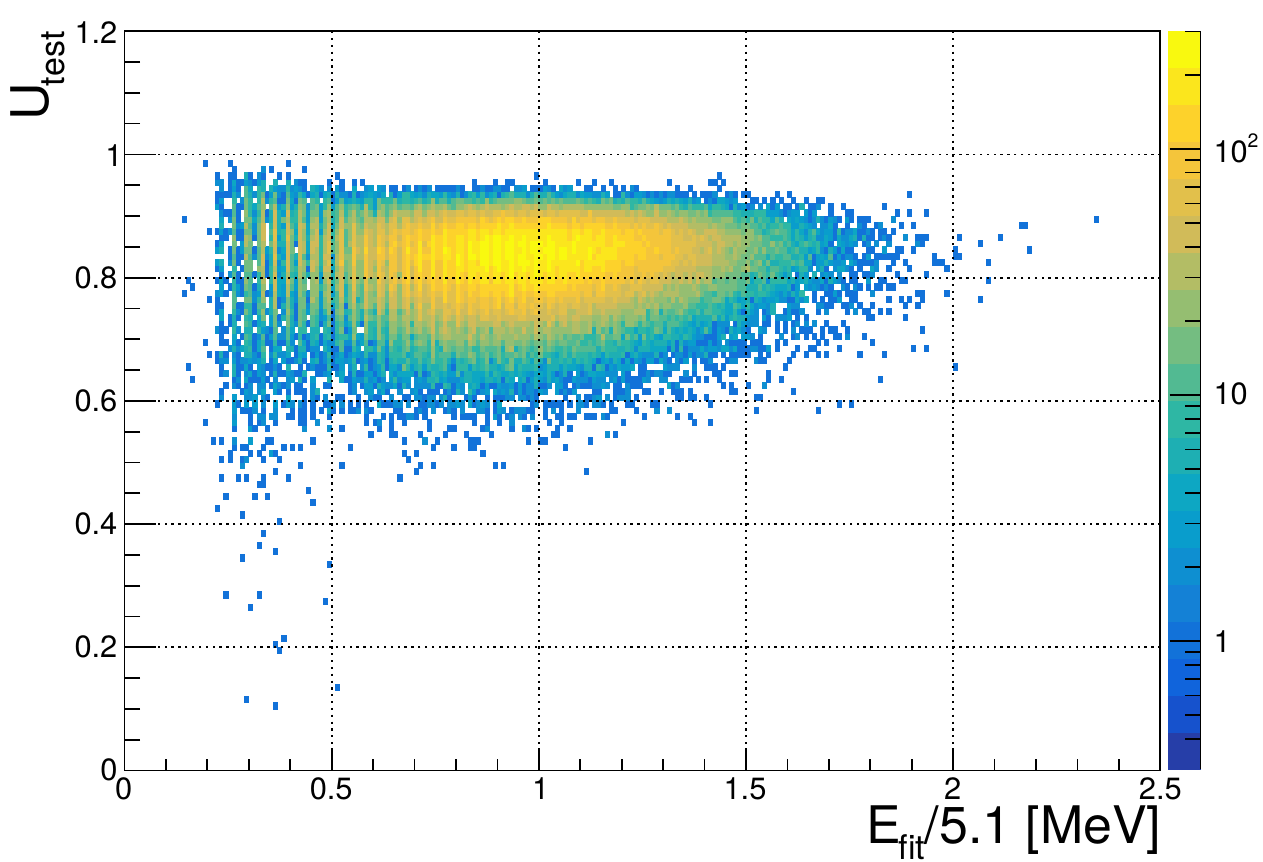
\includegraphics[width=8cm]{Utest_data_N16_107055.png}
		\subfigure[MC]{ 
			\begin{minipage}[t]{0.5\textwidth}
				\centering
				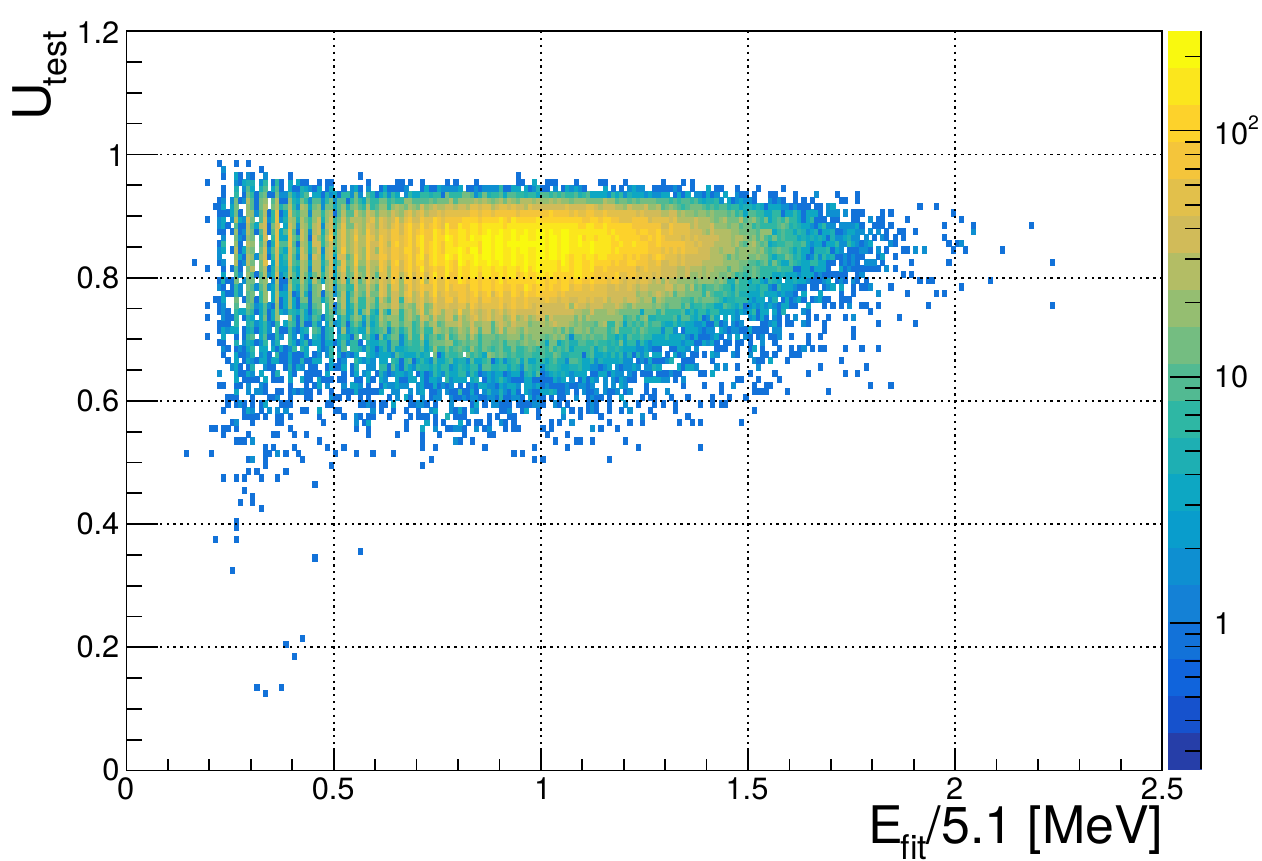
\includegraphics[width=7.5cm]{Utest_MC_N16_107055.png}
			\end{minipage}
		}
		\subfigure[data]{ 
			\begin{minipage}[t]{0.4\textwidth}
				\centering
				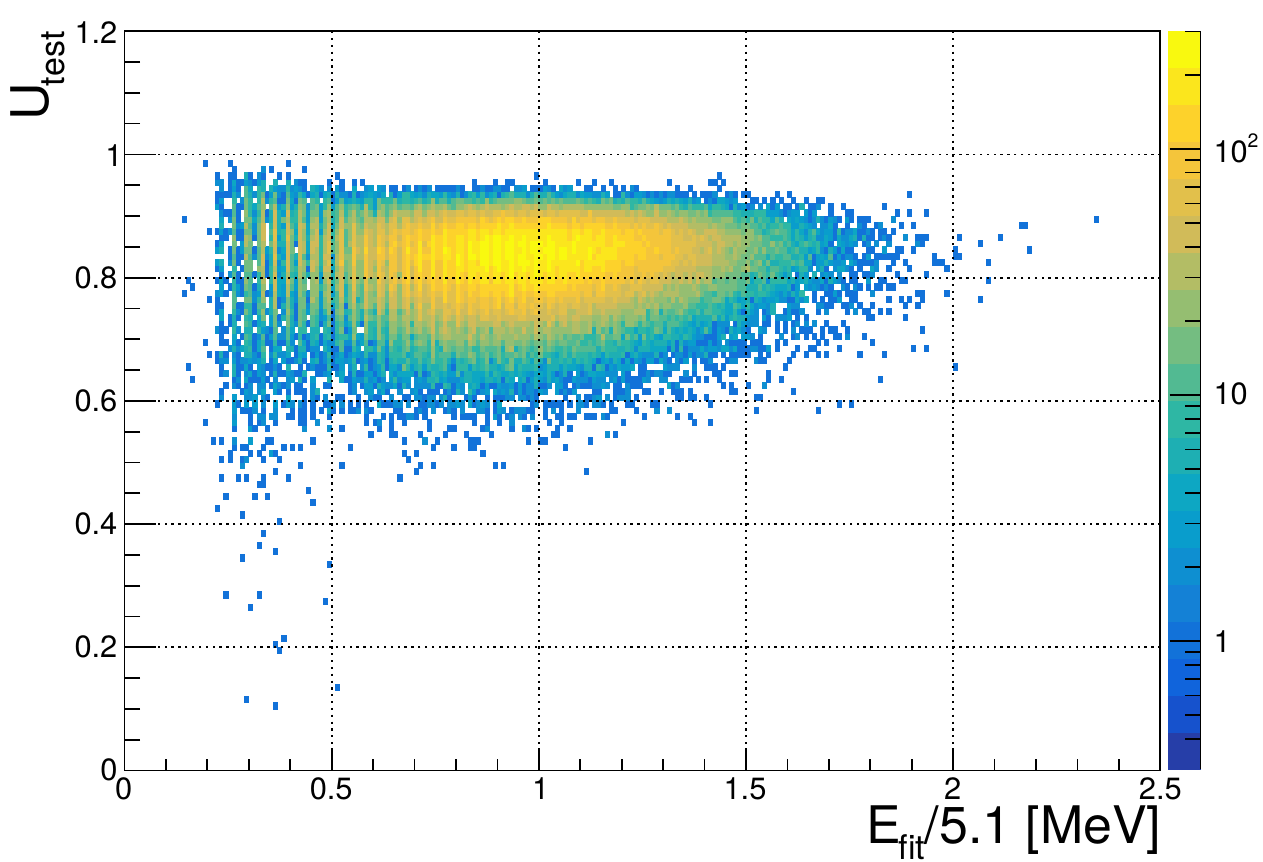
\includegraphics[width=7.5cm]{Utest_data_N16_107055.png}
			\end{minipage}
		}
		\caption{$^{16}$N central-run 107055, $U_{test}$ vs. $E_{fit}$/5.1 MeV.\label{energyFOM_Utest}}
		
	\end{figure}
	
	\item[$\bullet$] $G_{test}$: Fig.~\ref{energyFOM_Gtest} shows $G_{test}$ vs. energy biases. A cut of $0<G_{test}<1.9$ was suggested by the collaboration, which removes 0.01\% events for both MC and data.	
	
	\begin{figure}[!htb]
		\centering
		\subfigure[MC]{ 
			\begin{minipage}[t]{0.5\textwidth}
				\centering
				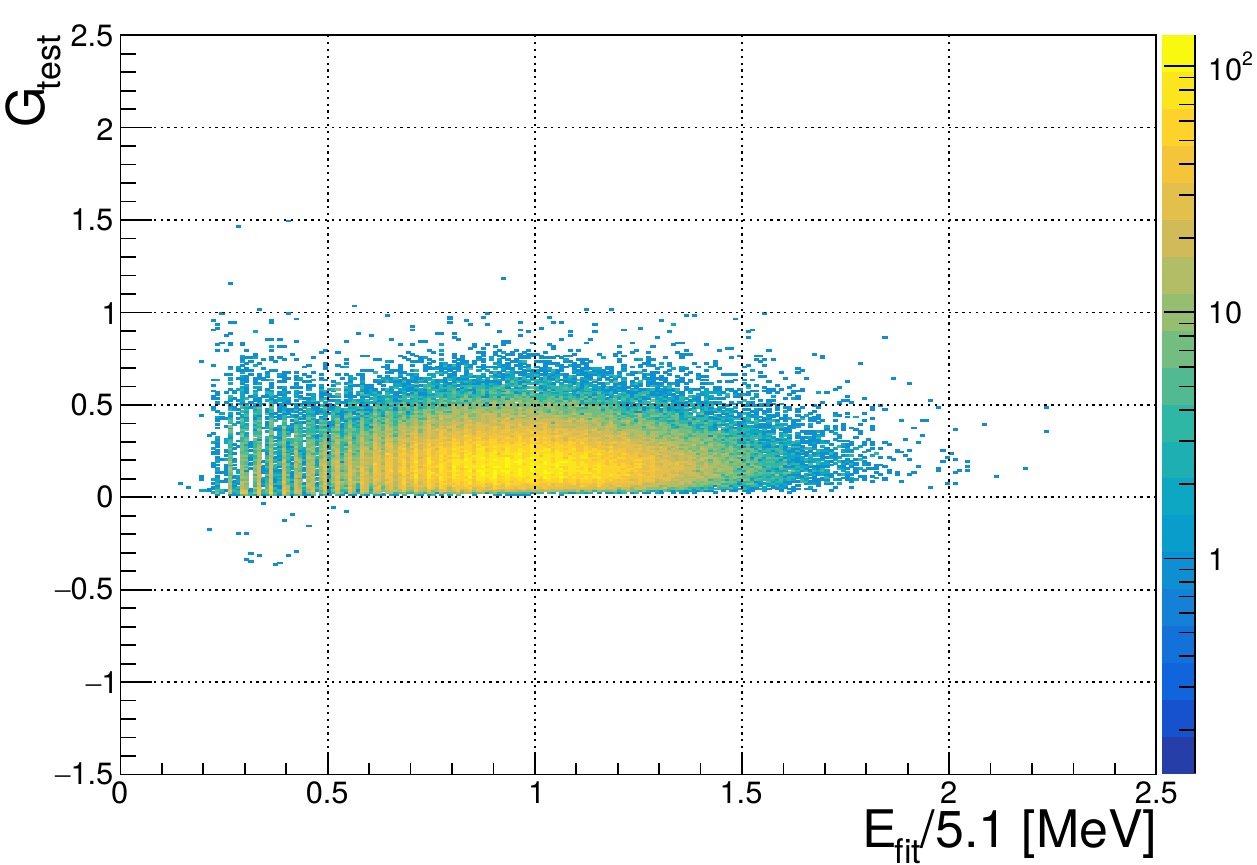
\includegraphics[width=7.5cm]{Gtest_MC_N16_107055.png}
			\end{minipage}
		}
		\subfigure[data]{ 
			\begin{minipage}[t]{0.4\textwidth}
				\centering
				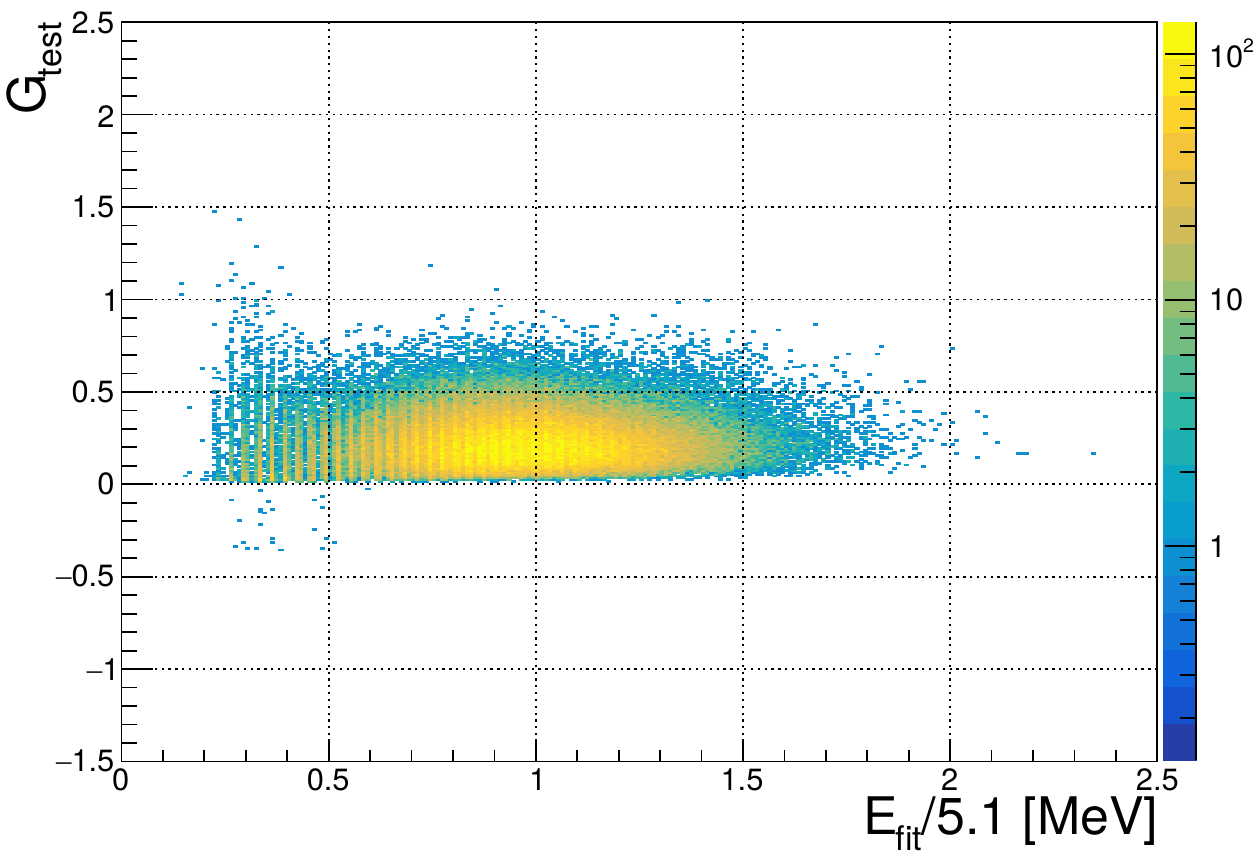
\includegraphics[width=7.5cm]{Gtest_data_N16_107055.png}
			\end{minipage}
		}
		\caption{$^{16}$N central-run 107055, $G_{test}$ vs. $E_{fit}$/5.1 MeV.\label{energyFOM_Gtest}}
	\end{figure}
	
	\item[$\bullet$]$Z_{factor}$:
	Fig.~\ref{energyFOM_Zfactor} shows $Z_{factor}$ vs. energy biases. A cut of $-11<Z_{factor}<1$ was suggested by the collaboration, which removes 0.13\% events for both MC and data.		
	\begin{figure}[!htb]
		\centering
		\subfigure[MC]{ 
			\begin{minipage}[t]{0.5\textwidth}
				\centering
				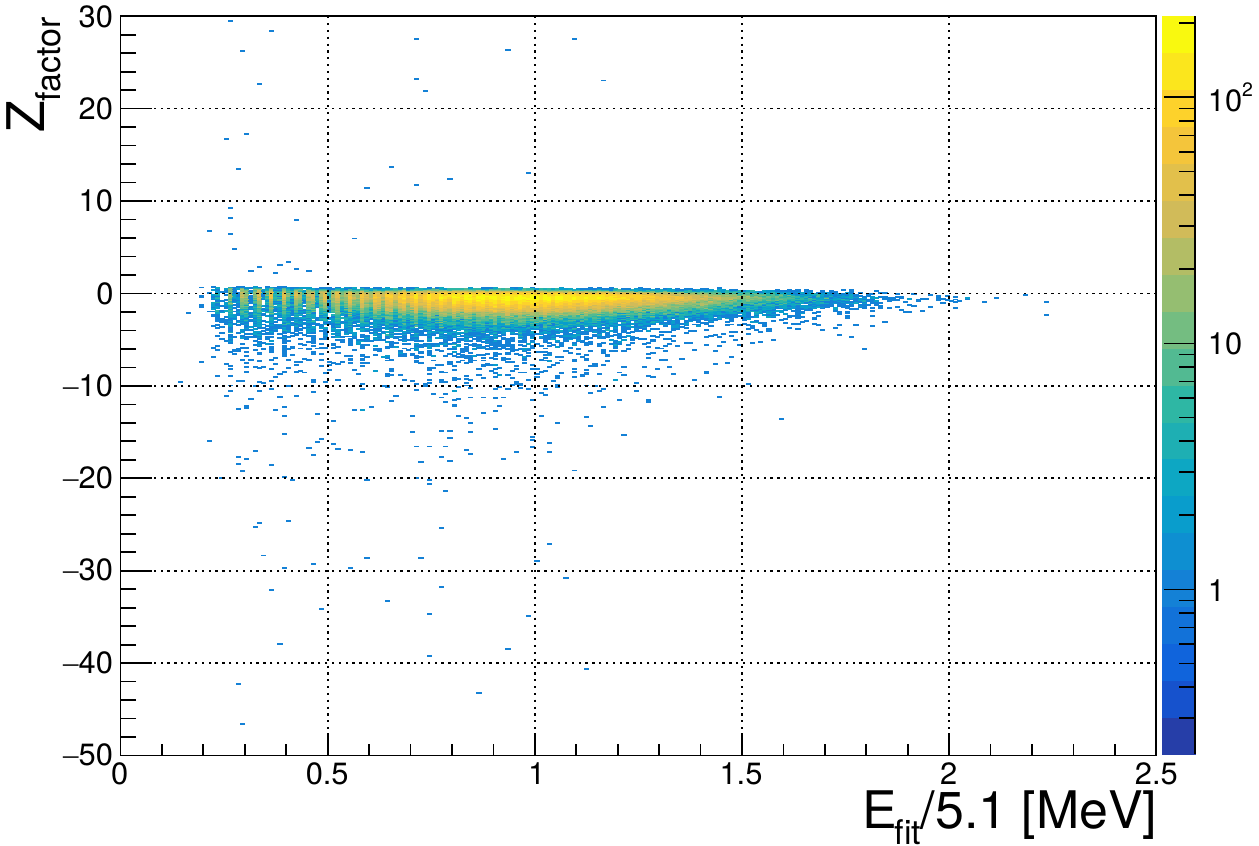
\includegraphics[width=7.5cm]{Zfactor_MC_N16_107055.png}
			\end{minipage}
		}
		\subfigure[data]{ 
			\begin{minipage}[t]{0.4\textwidth}
				\centering
				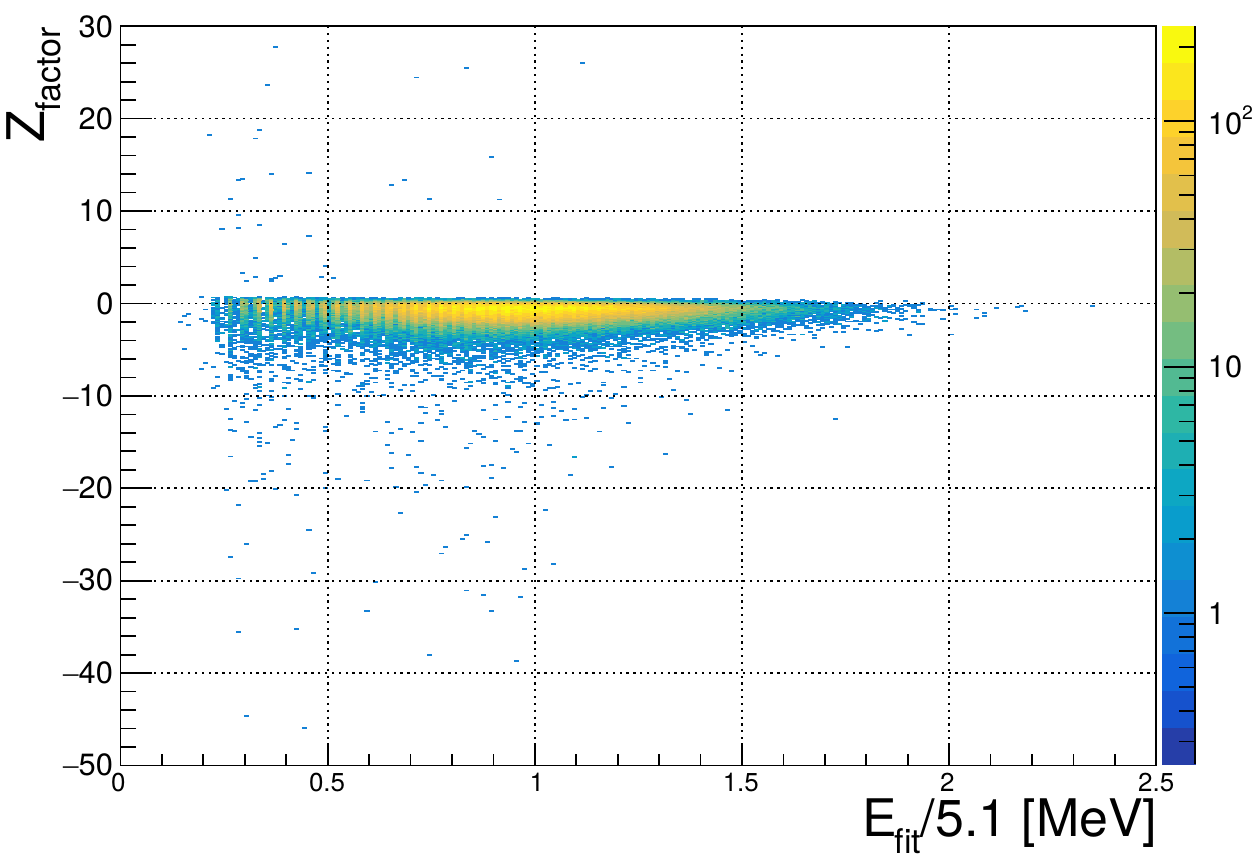
\includegraphics[width=7.5cm]{Zfactor_data_N16_107055.png}
			\end{minipage}
		}
		\caption{$^{16}$N central-run 107055, $Z_{factor}$ vs. $E_{fit}$/5.1 MeV.\label{energyFOM_Zfactor}}
		
	\end{figure}
	
	
\end{itemize}

All the cuts on the three energy FoM quantities remove 0.40\% events from MC and 0.37\% events from data. These cuts were also used in the water phase analysis in Chapter 6.

\subsubsection{Energy Resolution and Systematics}

The energy fitters for the water phase were applied to the $^{16}$N MC simulations and data. As described in Sect.~\ref{sect:energyFitter}, the energy fitters utilize the reconstructed vertex and direction of an event to convert the NHits value into the reconstructed energy. Before the energy reconstruction, a reconstruction threshold cut $\mathrm{NHits}>5$ was applied to both of the \texttt{RAT} and \texttt{MPW} fitters during the vertex and direction reconstructions. Then the energy fitters were applied to the results of the two fitters respectively. Fig.~\ref{fig:N16nhits} shows the spectra of the NHits of the $^{16}$N events in the central run 107055, comparing results from the MC and data. An $\mathrm{ITR}>0.55$ cut was also applied. The figure shows that the \texttt{MPW} fitter has more events in the $5<\mathrm{NHits}\leq 10$ region. In the region of $\mathrm{NHits}>10$, the two fitters generally match with each other, while the number of events of the MC is slightly less than the data, which is due to the biases in simulation models. 

\begin{figure}[htbp]
	\centering
	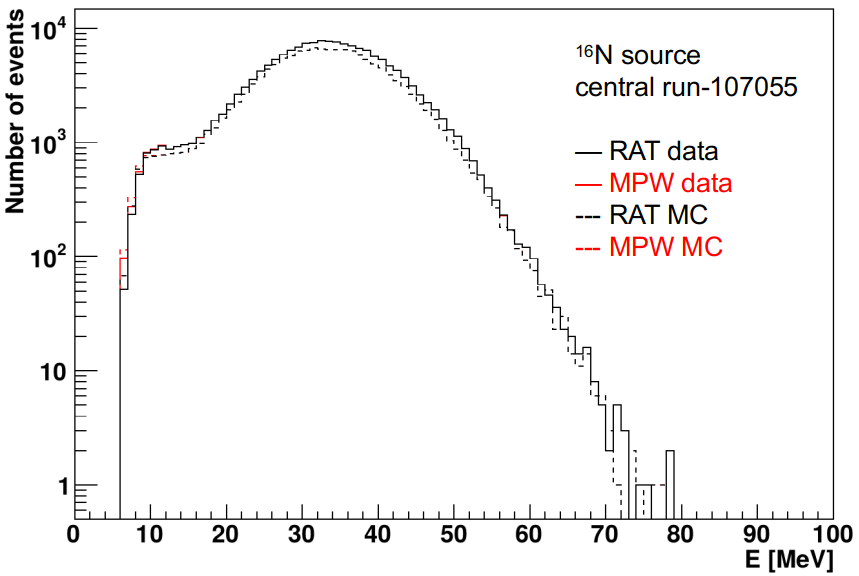
\includegraphics[width=10cm]{N16_nhits_107055.png}
	\caption[NHits spectra of the $^{16}$N central run 107055.]{NHits spectra of the $^{16}$N central run 107055. Dashed lines for the MC and solid lines for data; red for the MPW fitter results and black for the \texttt{RAT} results.\label{fig:N16nhits}}	
\end{figure}

Fig.~\ref{fig:N16energy} shows two examples for the reconstructed energy spectra of the $^{16}$N events. Cuts of $\mathrm{NHits}>5$ and $\mathrm{ITR}>0.55$ were applied. The upper plot shows the reconstructed energies of the $^{16}$N events in the central run 107055, comparing results from the MC and data. The reconstructed energies based on the results of the \texttt{RAT} and \texttt{MPW} fitters are also compared. The plot shows that the shapes of the spectra are very similar to the NHits case in Fig.~\ref{fig:N16nhits}, and the \texttt{MPW} fitter has more events around the $0.5<E<2$ MeV region. The lower plot shows the reconstructed energies for the run 106025 (the source position at (-186.0,254.0,-4999.9) mm), comparing the \texttt{MPW} results from the MC and data. The plot shows that when the source was close to the AV bottom, the performance of the energy reconstruction is still good.

\begin{figure}[htbp]
	\centering
   \subfigure[$^{16}$N run 107055]{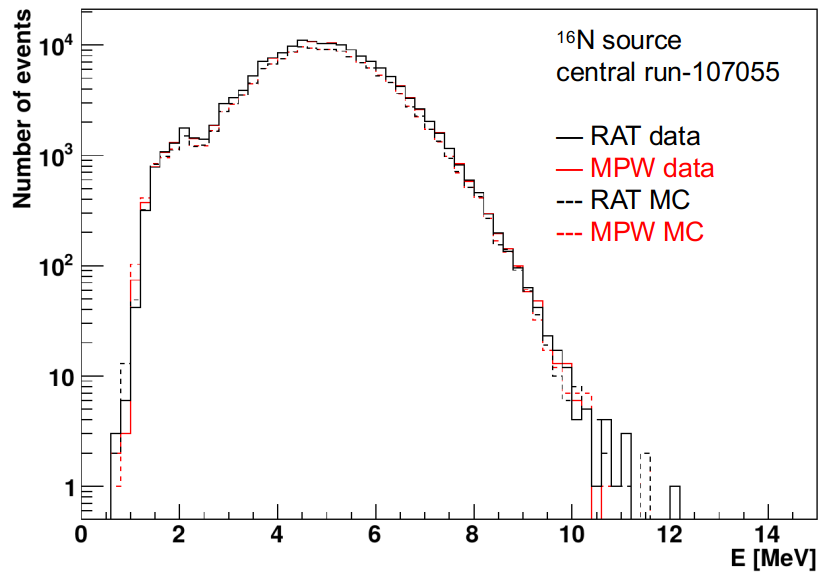
\includegraphics[width=8cm]{N16_reconE_107055.png}}
	\subfigure[$^{16}$N run 106925]{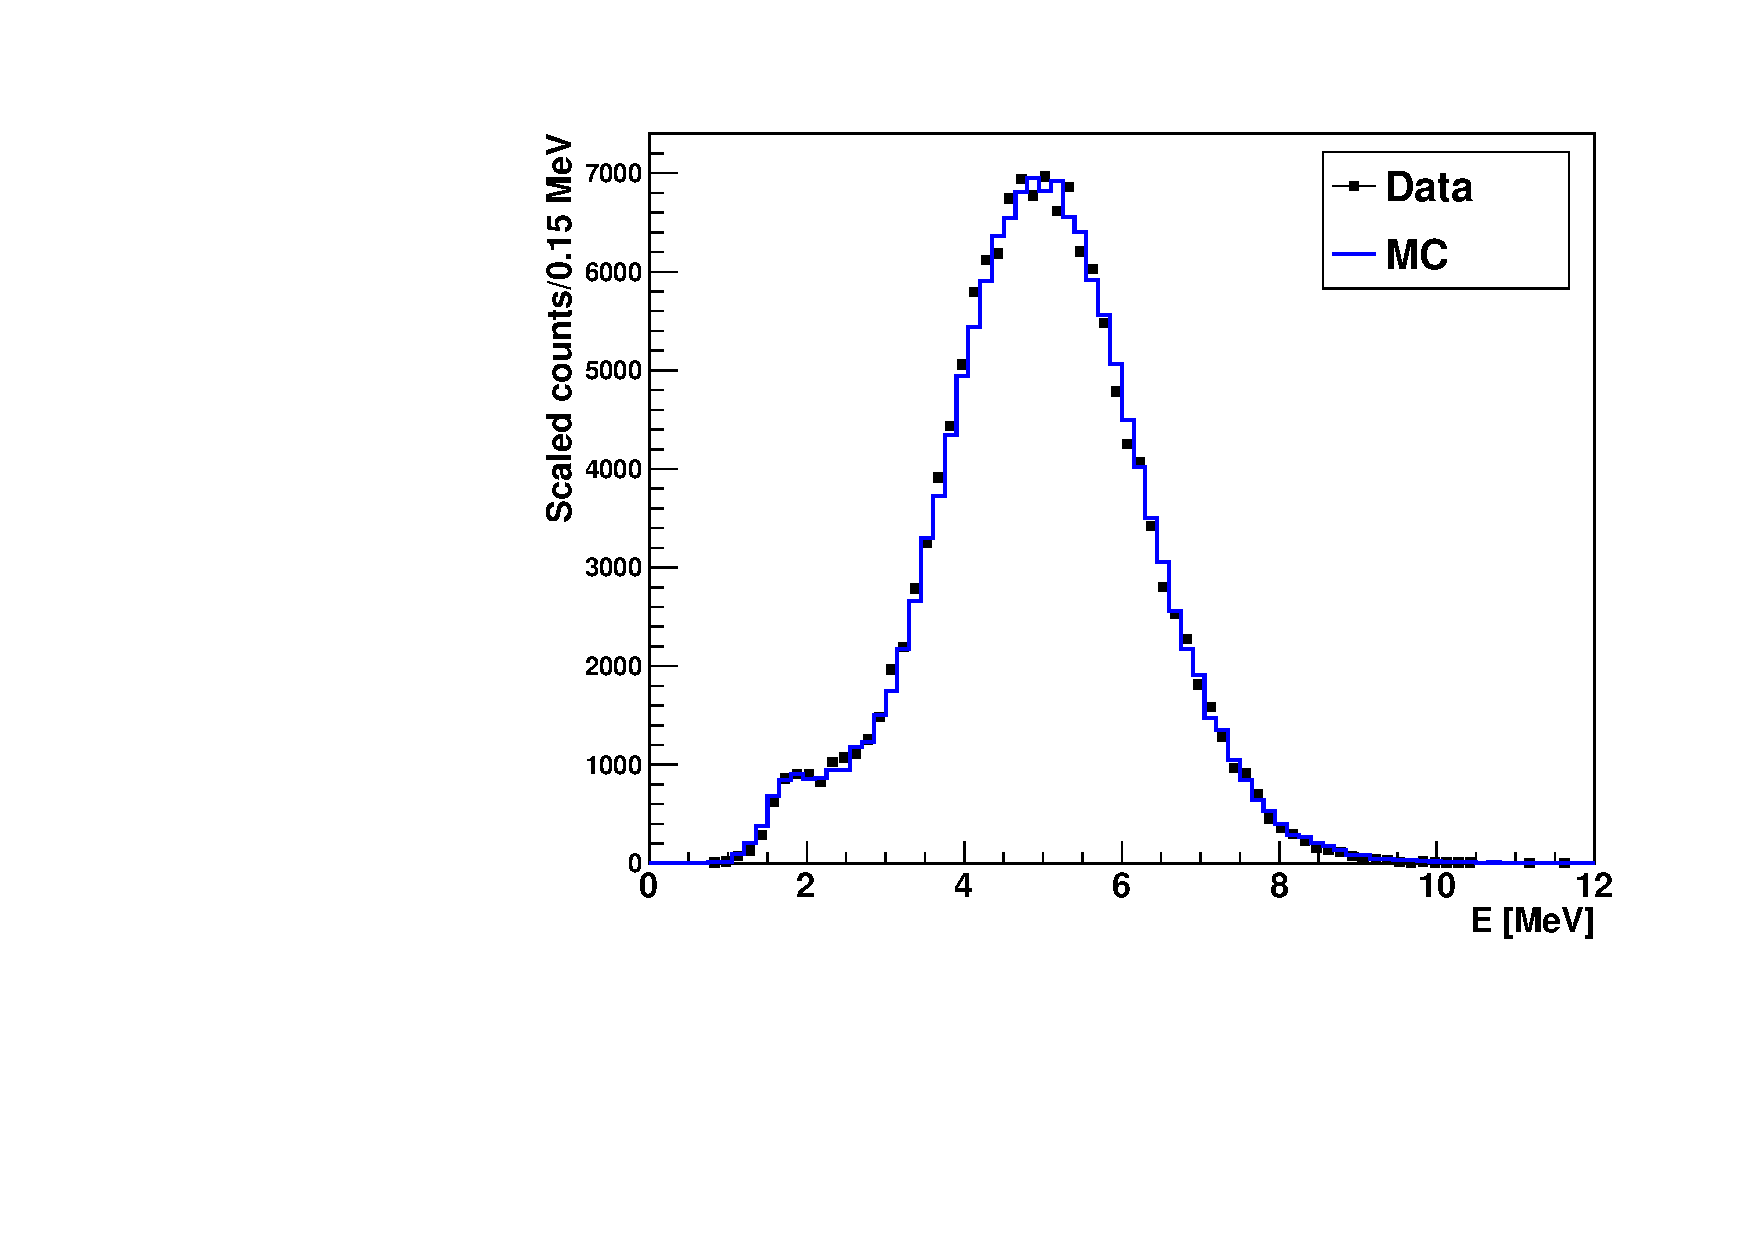
\includegraphics[width=8cm]{N16energyMPWcompare_106925.pdf}}
	\caption[Reconstructed energy spectra from the $^{16}$N central run 107055 and 106925.]{Reconstructed energy spectra from the $^{16}$N central run 107055 (upper) and 106925 (lower). For run 107055 (upper), the \texttt{MPW fitter} results and the \texttt{RAT} results are also compared. Dashed lines for the MC and solid lines for data; red for the \texttt{MPW fitter} results and black for the \texttt{RAT} results. For run 106925 (lower), the reconstructed data (black dots) are compared to the MC (blue line), both being \texttt{MPW fitter} results.\label{fig:N16energy}}
\end{figure}

\subsubsection{Energy Resolutions}
As mentioned in Sect.~\ref{sect:positionResol}, the $^{16}$N source can be considered as an electron source with a known spatial distribution. The $\gamma$-particles emitted from the source interact with the detector materials via different processes and produce electrons with various energies. Fig.~\ref{fig:N16nhitsSimu} shows the spectra of electron energies derived from the simulations of the $^{16}$N central run 107055. It shows the contributions from three processes: Compton scattering, pair production, and photoelectric absorption. Among these contributions, Compton scattering is dominant, while photoelectric absorption is negligible. The $\gamma$-particles transfer energies to electrons, while the energy reconstruction for SNO+ is based on electron equivalent energy (unit: MeVee), the source energy must be mapped to electron equivalent energy \cite{morganThesis}. 

\begin{figure}[htbp]
	\centering
	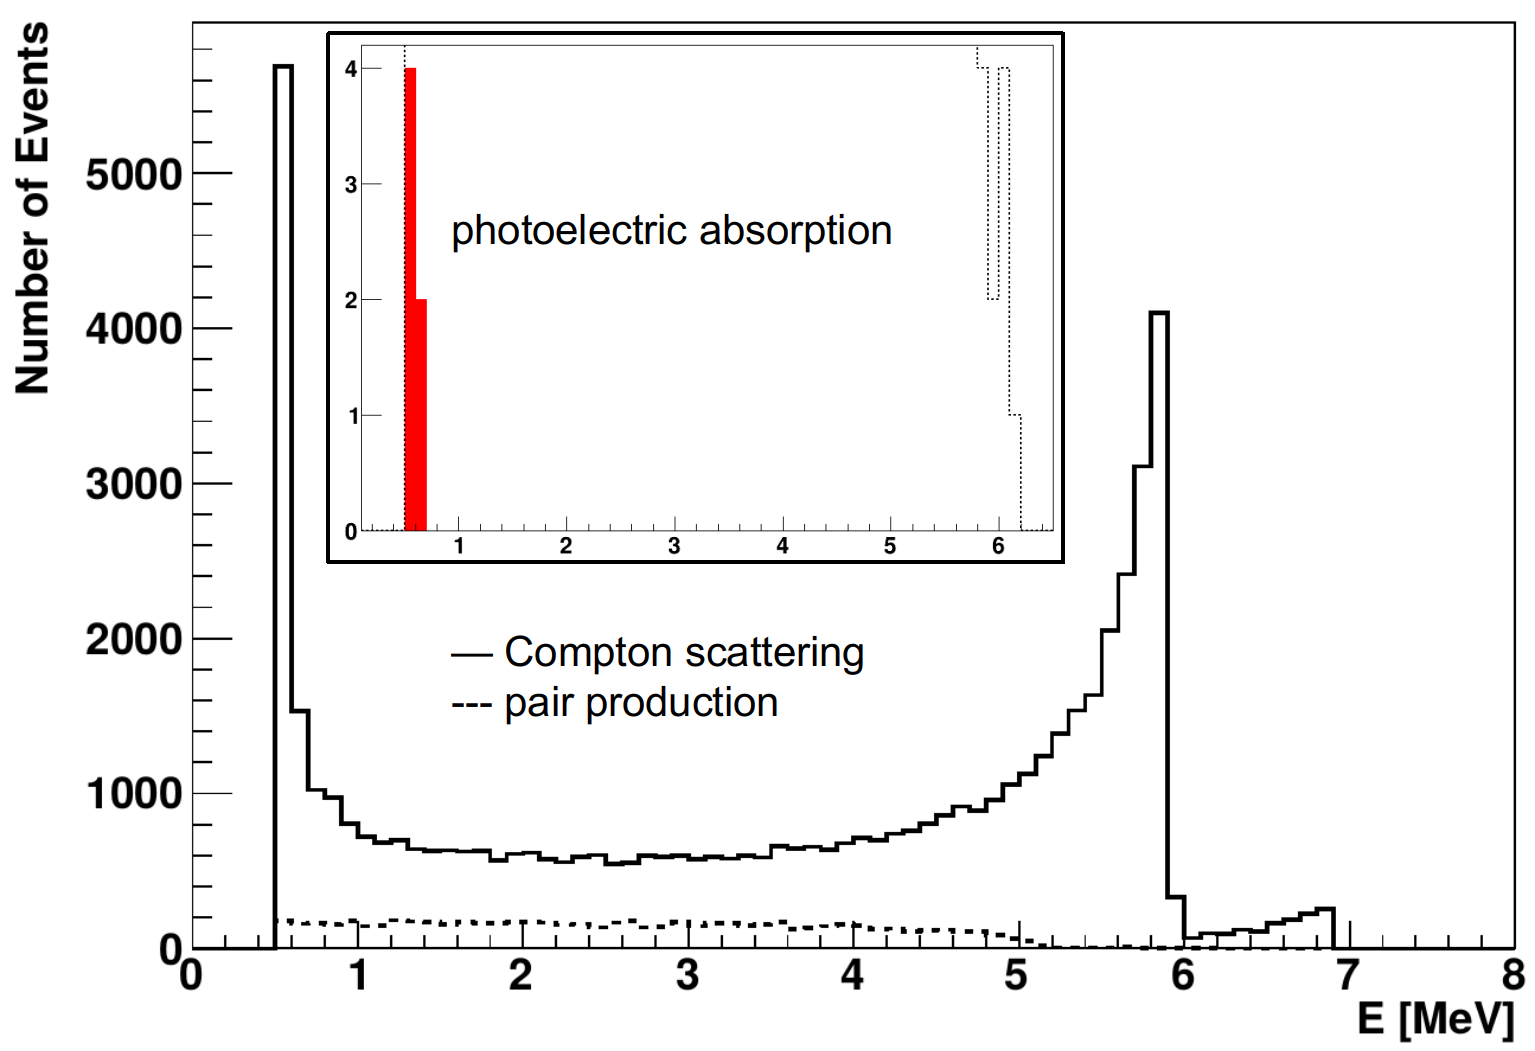
\includegraphics[width=12cm]{N16_MCenergySpectrum.png}
	\caption[Simulated electron energy spectra for different processes.]{Simulated electron energy spectra for different processes, extracted from $10^5$ MC simulations of $^{16}$N central run 107055. Contributions from three processes: Compton scattering, pair production, and photoelectric absorption are shown.\label{fig:N16nhitsSimu}}
\end{figure}

Following the methods described in Refs.~\cite{morganThesis,waterunidoc}, a map that relates the number of Cherenkov photons to the electron energy is created by simulating electron events with different energies at the detector center, as shown in the upper plot of Fig.~\ref{N16energyMap}. By looking up the map and applying linear interpolation, the number of the photons created from the $^{16}$N source can be converted into an effective or apparent electron energy spectrum ($P_\mathrm{source}(T_e)$)\cite{waterunidoc}. Fig.~\ref{N16energyMap} (b) shows the effective electron spectrum of $^{16}$N central run 107055.

%%The apparent energy spectrum $P_{source(Te) is generated with RAT and relates the 16N $\gamma$ energy to apparent energy by considering Cherenkov photon production, Compton scattering, pair production, and energy
%%deposition in the source container.

%%the source energy must be mapped to electron-equivalent energy

\begin{figure}[htbp]
	\centering
    \subfigure[]{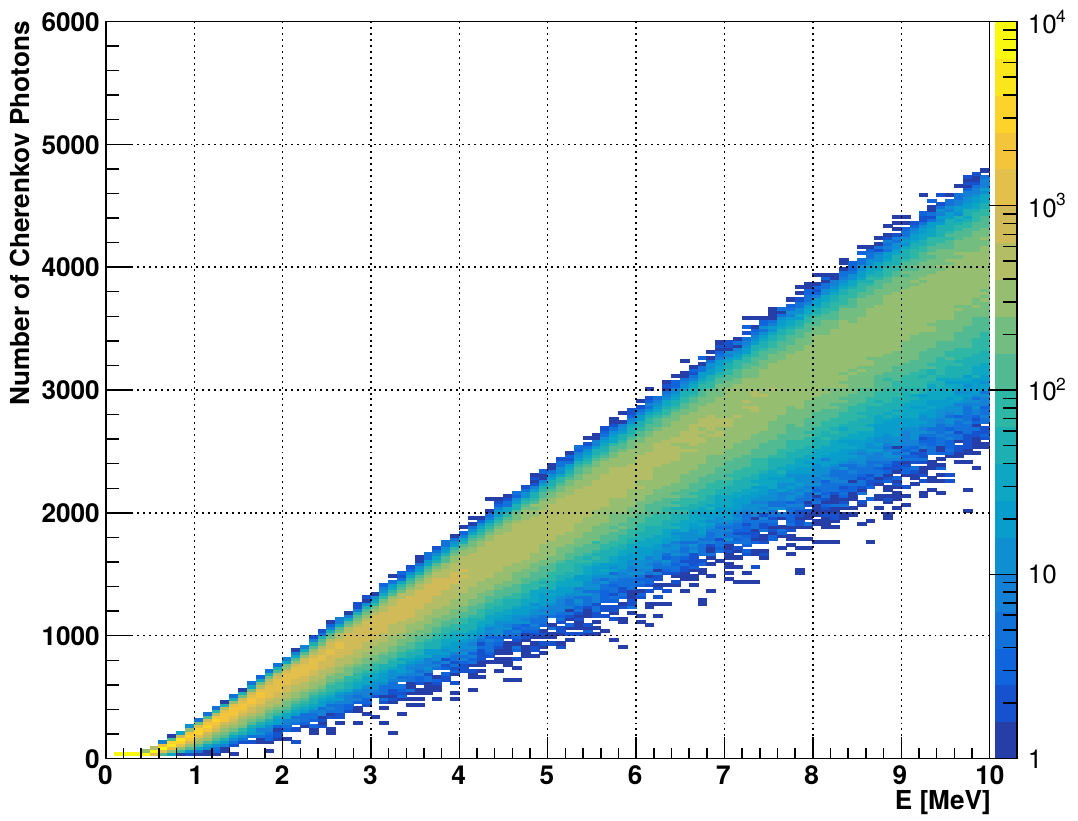
\includegraphics[width=8cm]{2dmap_EvsNphoton.png}}
	\subfigure[]{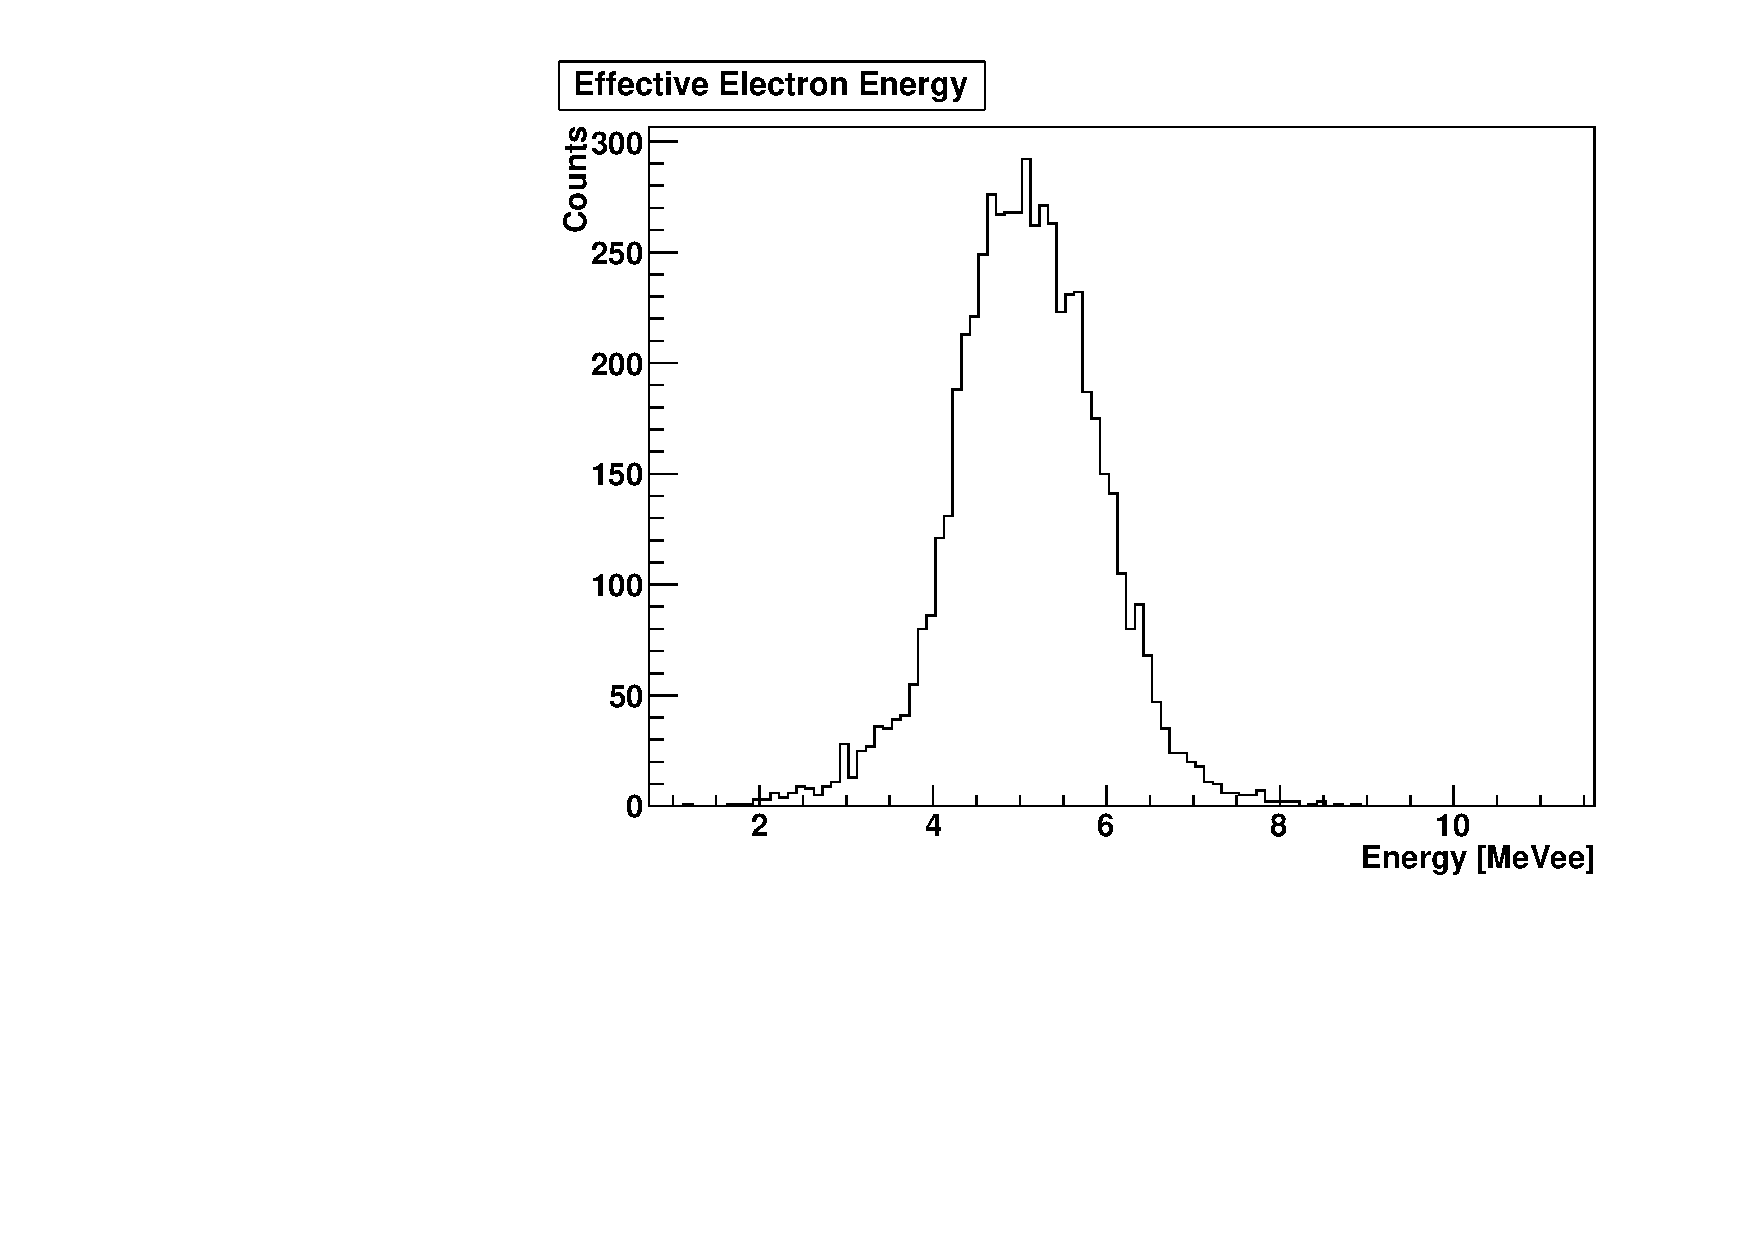
\includegraphics[width=8cm]{N16_run107055_apparentEnergy.pdf}}
	\caption[Converting number of photons to effective electron spectrum.]{Converting number of photons to effective electron spectrum. (a): A 2D map of Electron energy vs number of Cherenkov photons. (b):	Effective electron spectrum of $^{16}$N central run 107055.\label{N16energyMap}}
\end{figure}

To obtain the energy reconstruction resolutions, the reconstructed energy spectrum $P(T_{eff})$ is fitted with the energy resolution function defined as \cite{waterunidoc}:

\begin{equation}
P(T_{eff})=N\int P_\mathrm{source}(T_e)\frac{1}{\sqrt{2\pi}\sigma_E} \; \exp \left[ -\frac{[(1+\delta_E)T_{eff}-T_e]^2}{2\sigma_E^2} \, \right] \, ,
\end{equation}
where the predicted apparent energy spectrum, $P_\mathrm{source}(T_e)$, is convolved with a Gaussian resolution function. In the Gaussian function, $\sigma_E$ is the detector resolution and $\sigma_E = b\sqrt {T_{eff}}$, where $b$ is the energy resolution parameter and $\delta_E$ is the energy scale parameter. $P_\mathrm{source}(T_e)$ is the apparent energy spectrum.

Before fitting the reconstructed energy spectrum with the energy resolution function, the following cuts were applied (on both the data and MC): 

\begin{itemize}
\item the position FoM cut $scaleLogL>10$ and the energy FoM cuts mentioned in the previous sections, i.e. $0<G_{test}<1.9$, $U_{test}<0.95$ and $-11<Z_{factor}<1$;

\item cuts $\mathrm{NHit}>5$, $\mathrm{ITR}>0.55$ and $-0.12<\beta_{14}<0.95$, used to remove instrumental backgrounds;

\item a conditional distance cut, $|\vec{X}_{fit}-\vec{X}_{src}|>700~$mm was suggested by Refs.~\cite{leta,waterunidoc} to remove shadow effects when the events are close to the source container. The conditional cut is applied as follows: an event reconstructed within the $700~ \mathrm{mm}$ proximity to the source is retained only if its direction $\vec{u}_{fit}$ is within 45$^\circ$ of the vector from the source to its vertex, i.e., if $\sqrt2/2<\vec{u}_{true}\cdot \vec{u}_{fit}<1$.

\end{itemize}

Fig.~\ref{fig:EvsBeta14} shows the relationship between the reconstructed energies ($E_{fit}$) and $\beta_{14}$ values, comparing the \texttt{MPW} and \texttt{RAT} results from the MC and data respectively. 

\begin{figure}[htbp]
	\centering
	\subfigure[\texttt{RAT} data]{ 
		\begin{minipage}[t]{0.4\textwidth}
			\centering
			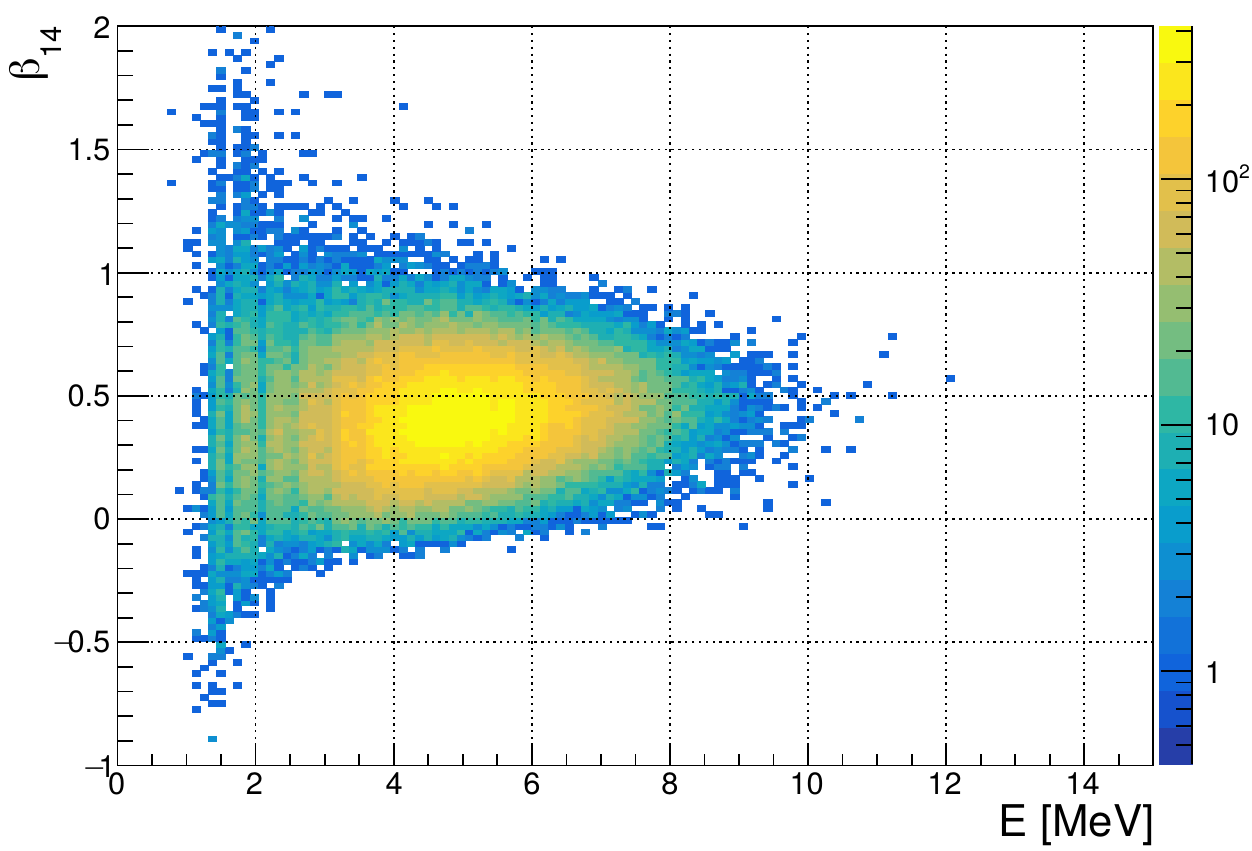
\includegraphics[width=6cm]{N16_rat_data_EvsBeta14.png}
		\end{minipage}
	}
	\subfigure[\texttt{RAT} MC]{ 
		\begin{minipage}[b]{0.4\textwidth}
			\centering
			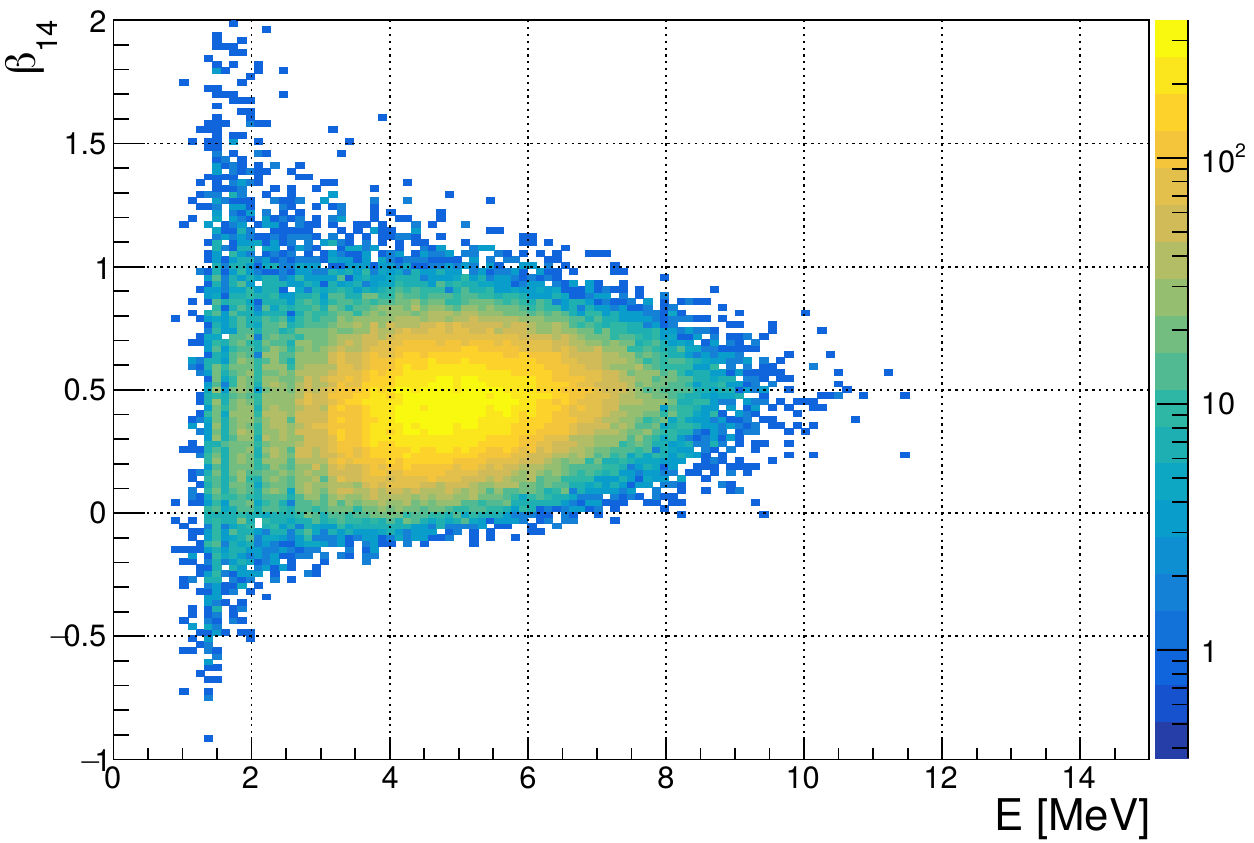
\includegraphics[width=6cm]{N16_rat_mc_EvsBeta14.png}
		\end{minipage}
	}
	\subfigure[\texttt{MPW} data]{ 
		\begin{minipage}[t]{0.4\textwidth}
			\centering
			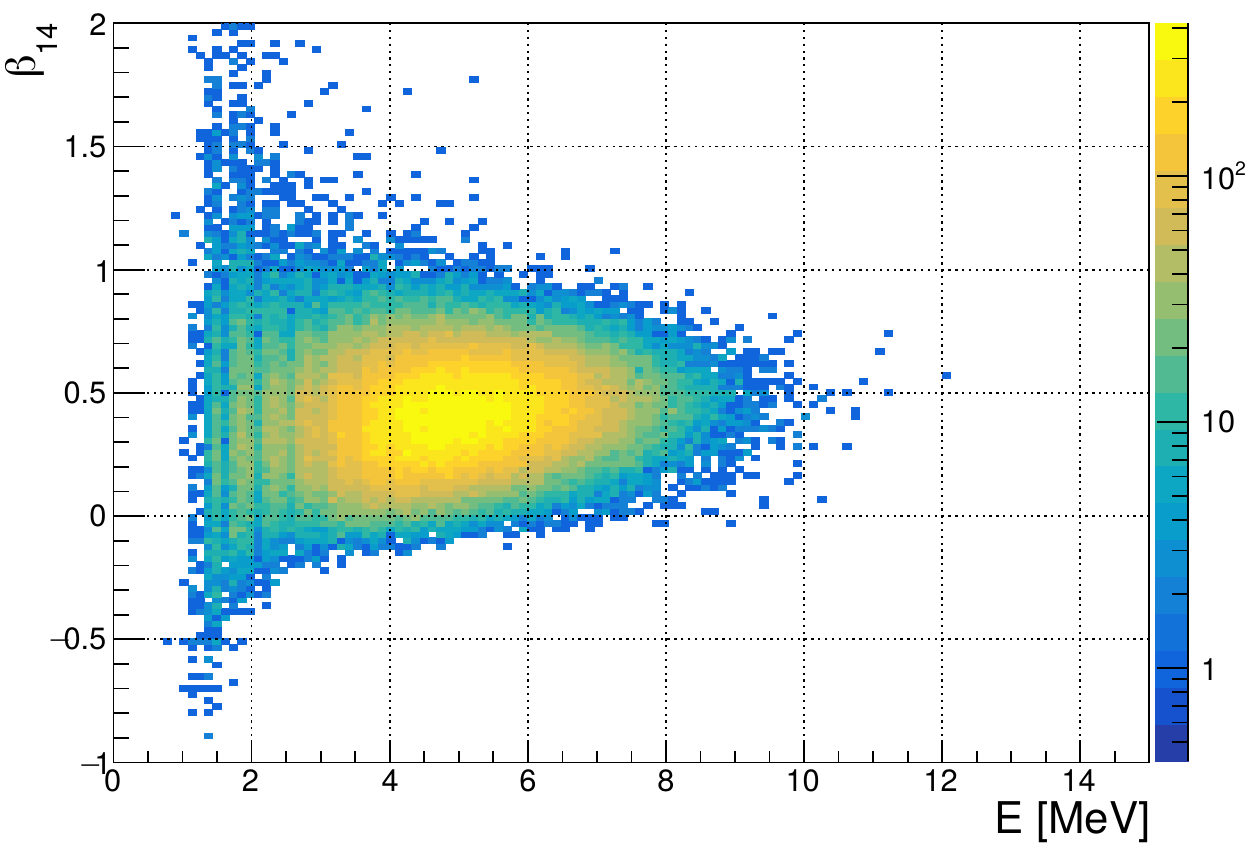
\includegraphics[width=6cm]{N16_MPW_data_EvsBeta14.png}
		\end{minipage}
	}
	\subfigure[\texttt{MPW} MC]{ 
		\begin{minipage}[t]{0.4\textwidth}
			\centering
			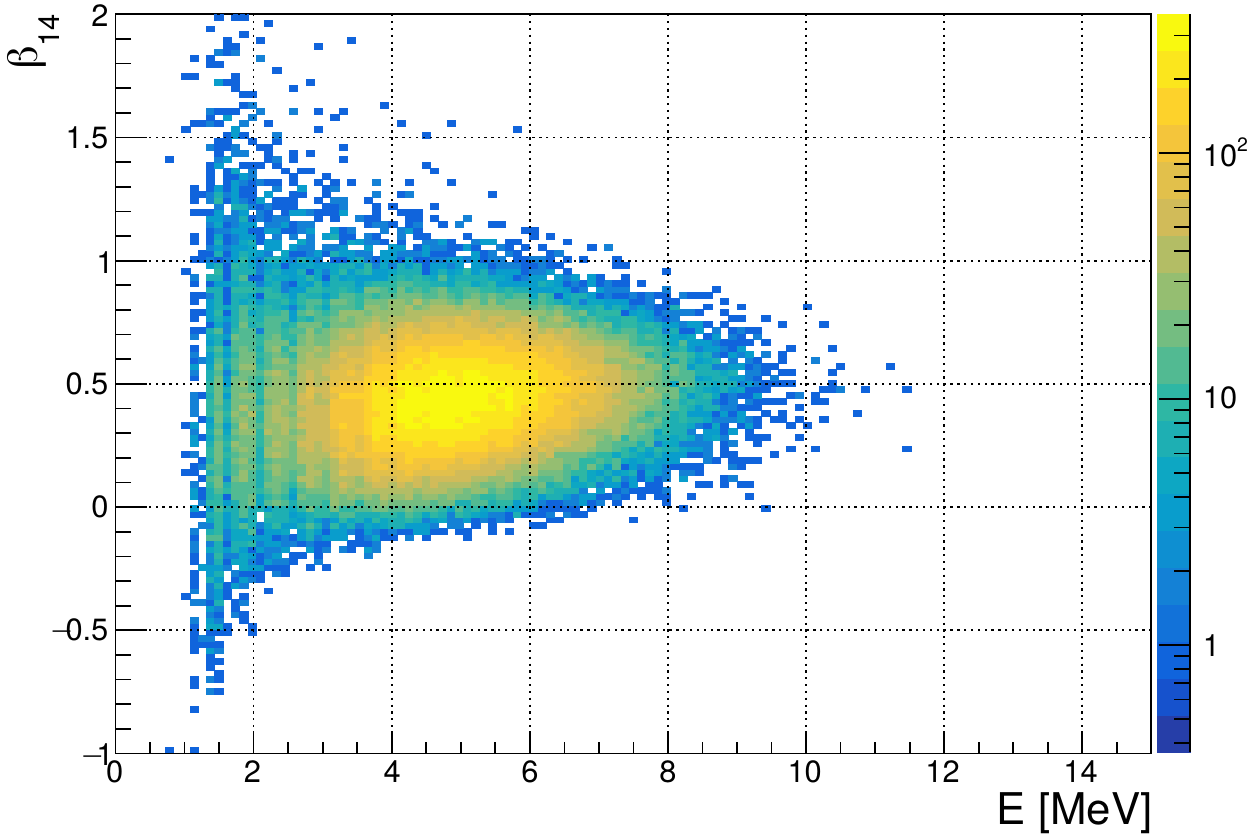
\includegraphics[width=6cm]{N16_MPW_mc_EvsBeta14.png}
		\end{minipage}
	}
	\caption[$E_{fit}$ vs $\beta_{14}$ for the data and MC.]{$E_{fit}$ vs $\beta_{14}$ for the data and MC. Both the \texttt{RAT} (a, b) and the \texttt{MPW} (c, d) results are shown.\label{fig:EvsBeta14}}
\end{figure}

A fit range of [3.5, 6.0]~MeV was suggested by Ref.~\cite{waterunidoc} to avoid including poorly reconstructed events due to the trigger inefficiency. Fig.~\ref{fittedEnergyResol} shows the energy resolution function fitted with the reconstructed energy spectrum of the $^{16}$N central run-107055 data, after applying the cuts mentioned above.
\begin{figure}
	\centering
	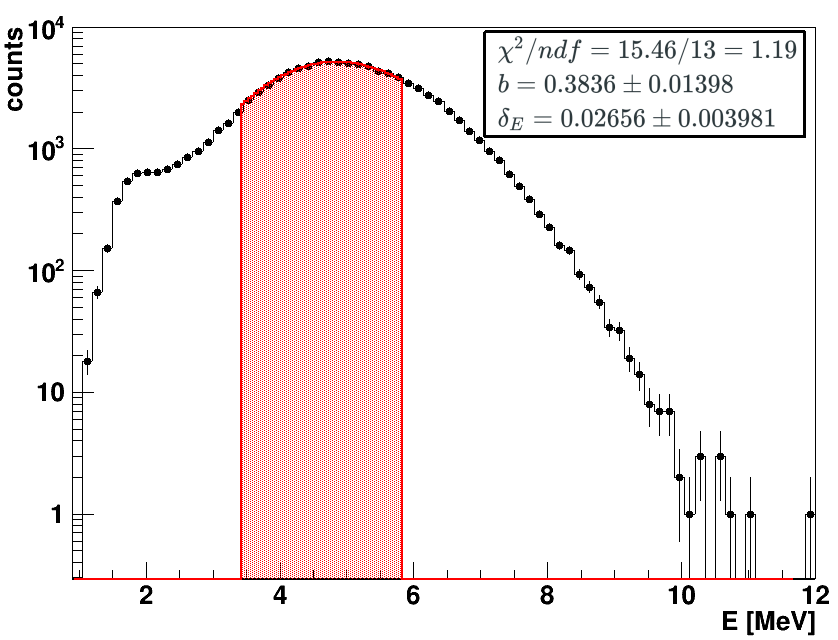
\includegraphics[width=8cm]{N16data_energy_fitted_107055.png}
	\caption[The reconstructed energy spectrum fitted with resolution function.]{The reconstructed energy spectrum of central run 107055 data, fitted with the resolution function (red).\label{fittedEnergyResol}}
\end{figure}

For all the internal scans, Fig.~\ref{fig:EscaleVsR} and Fig.~\ref{fig:EresolVsR} show the energy scale ($\delta_E$) and energy resolution ($b$) as a function of the source manipulator's radial position. Both the data and MC are shown.
\begin{figure}
	\centering
    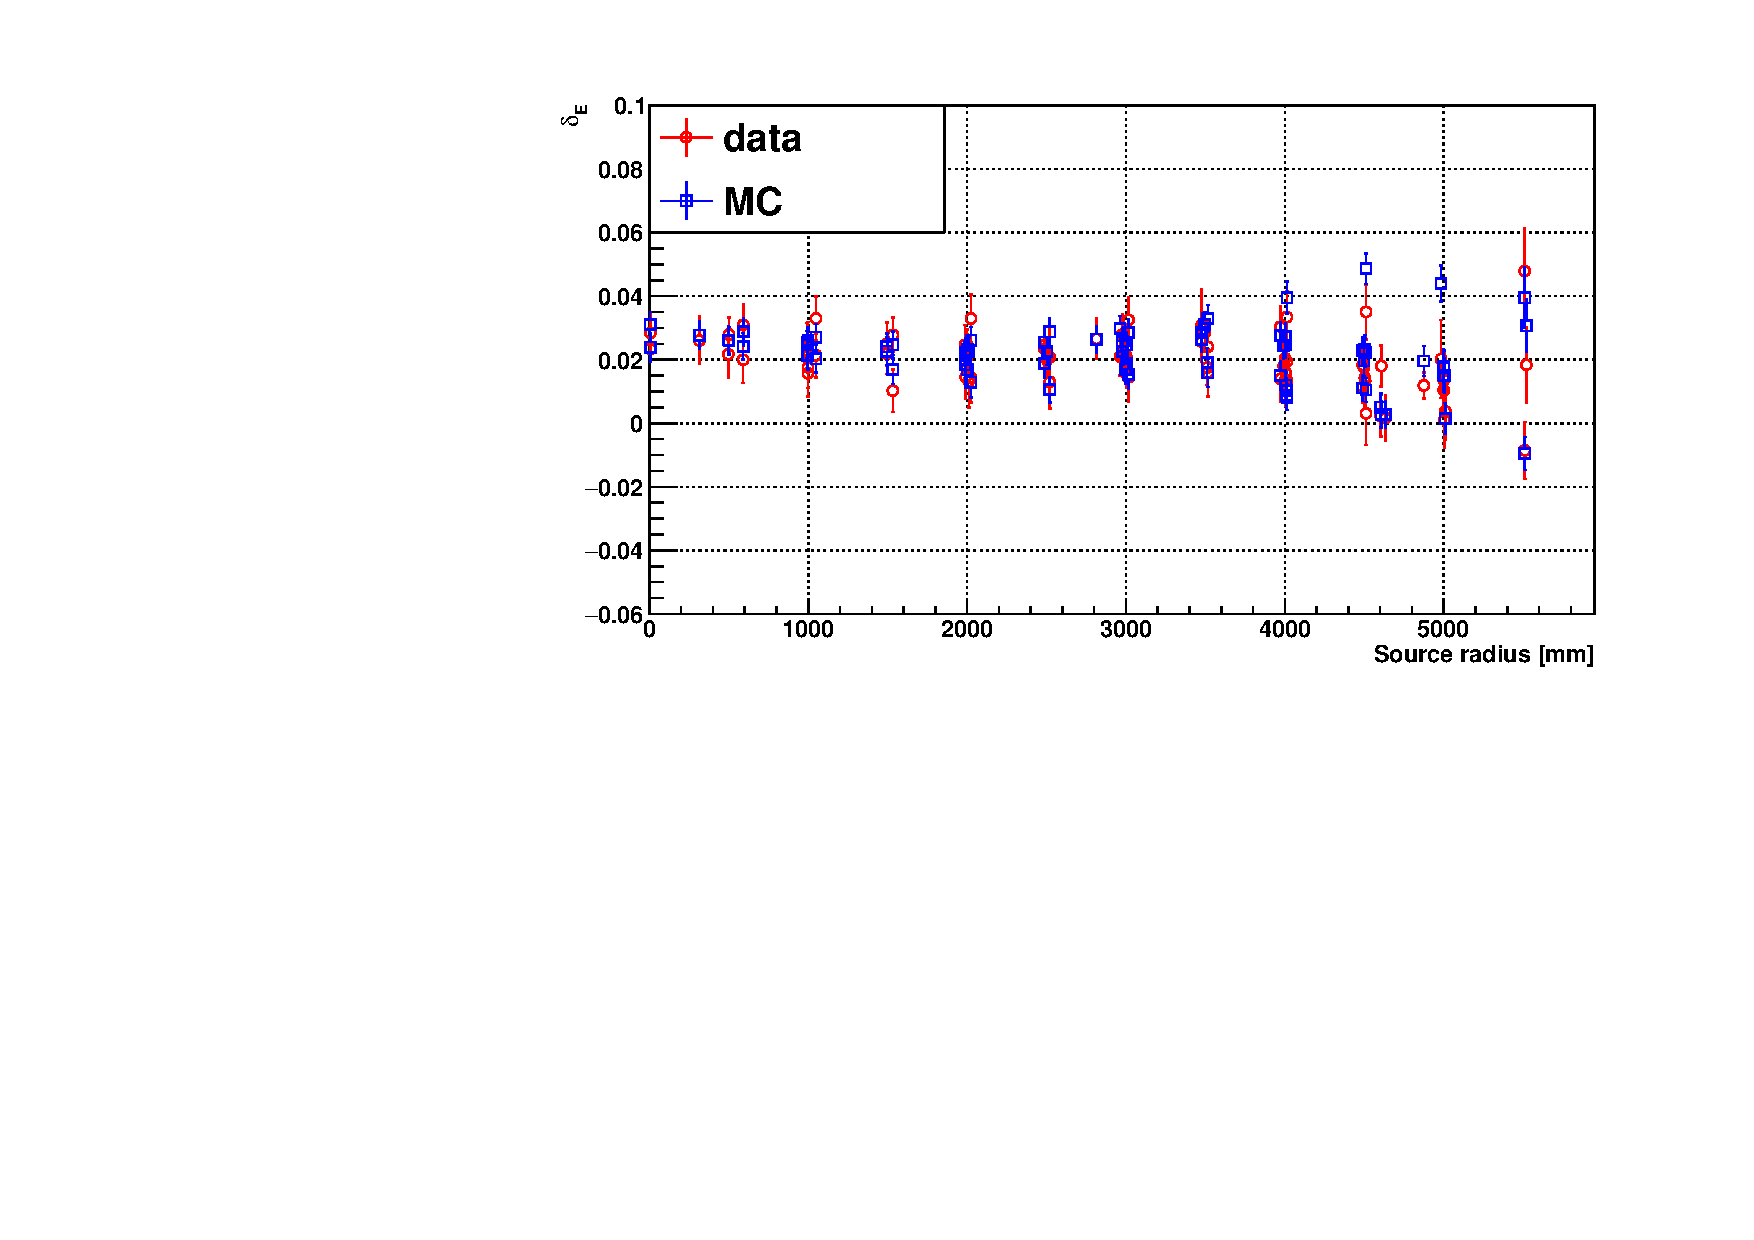
\includegraphics[width=12cm]{EscaleVsSrcRadius.pdf}
	\caption[Fitted energy scales as a function of the source manipulator's radial position.]{Fitted energy scales ($\delta_E$) as a function of the source manipulator's radial position. Red circles for data and blue squares for the MC.	\label{fig:EscaleVsR}}
\end{figure}

\begin{figure}
	\centering
	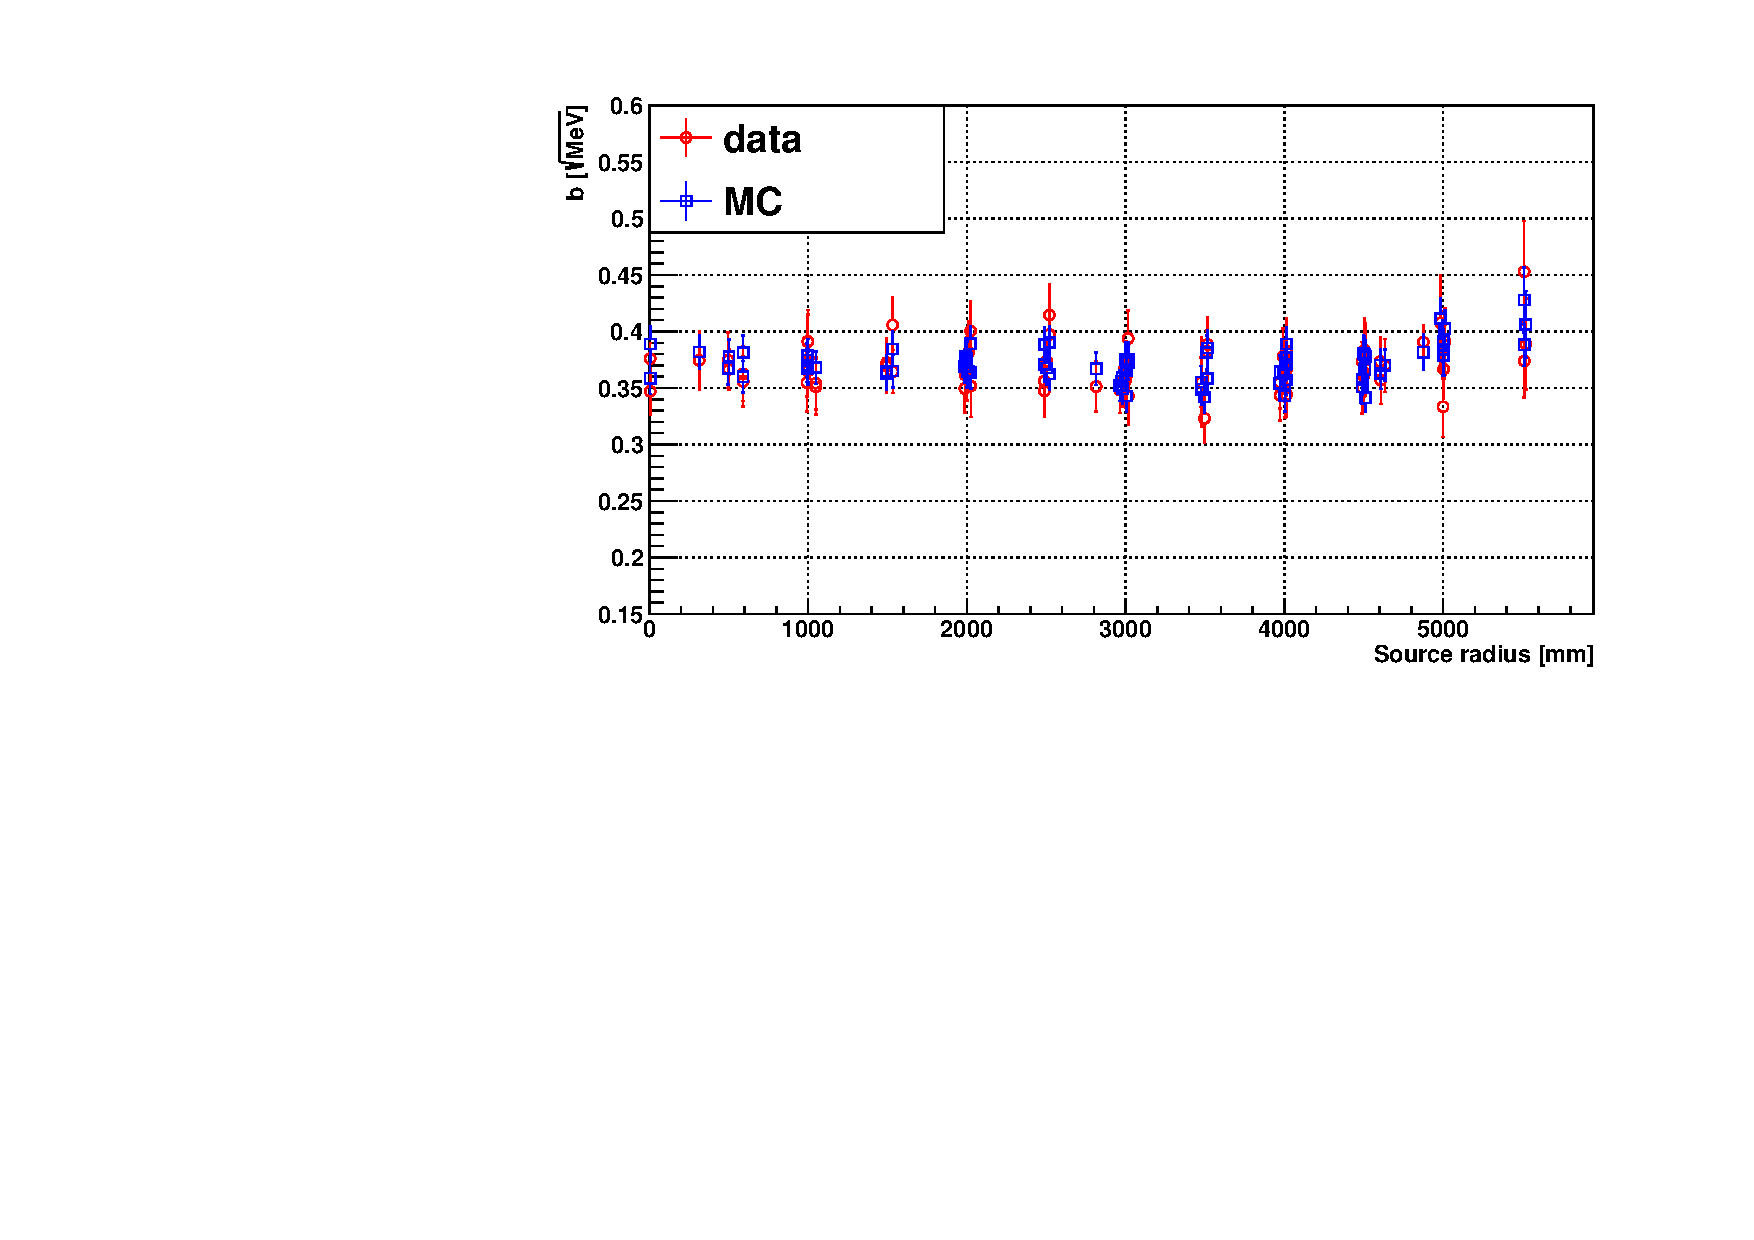
\includegraphics[width=12cm]{EresolVsSrcRadius.pdf}
	\caption[Fitted energy resolutions ($b$) as a function of the source manipulator's radial position.]{Fitted energy resolutions ($b$) as a function of the source manipulator's radial position. Red circles for data and blue squares for the MC.	\label{fig:EresolVsR}}
\end{figure}

\subsubsection{Energy Uncertainties}\label{sect:eneryUncertianties}

By comparing the differences between data and MC, the uncertainties of the energy scale $\delta_E$ and resolution $b$ are calculated as:
\begin{equation}
\Delta^2_{\delta}= (\delta_{data}-\delta_{MC})^2+\mathrm{Error}^2_{\delta,data}+\mathrm{Error}^2_{\delta,MC}\; ,
\end{equation}
where $\delta=b$ or $\delta_E$, and $\Delta_b=\sqrt{\Delta^2_{b}}$ since the resolution is always positive; while $\Delta_{\delta_E}=\pm\sqrt{\Delta^2_{\delta_E}}$. The fit errors in data and MC were also included in the uncertainties. Taking the $^{16}$N scan runs within $r<6~$m, the averaged uncertainties are: $\overline{\Delta_{\delta_E}}=0.0107$ and $\overline{\Delta_{b}}=0.0369$. For the $^{16}$N scan runs within $r<5.5~\mathrm{m}$, which is the fiducial volume of the solar neutrino analysis mentioned in Chapter 6, $\overline{\Delta_{\delta_E}}=0.0100$ and $\overline{\Delta_{b}}=0.0320$.

To apply the energy scale systematics, the reconstructed energy $E_{fit}$ is smeared by $E'_{fit}=(1\pm\Delta_{\delta_E}) \; E_{fit}$, where the ``$+$" sign is for scaling up the energy while ``$-$" is for scaling down. Fig.~\ref{fig:EscaleSmear} shows the effects of smearing the energy scales on the reconstructed energy spectrum of the $^{16}$N central run 107055. It is obvious that scaling up the $E_{fit}$ widens the $E_{fit}$ spectrum while scaling down the $E_{fit}$ narrows the spectrum. 

\begin{figure}
	\centering
	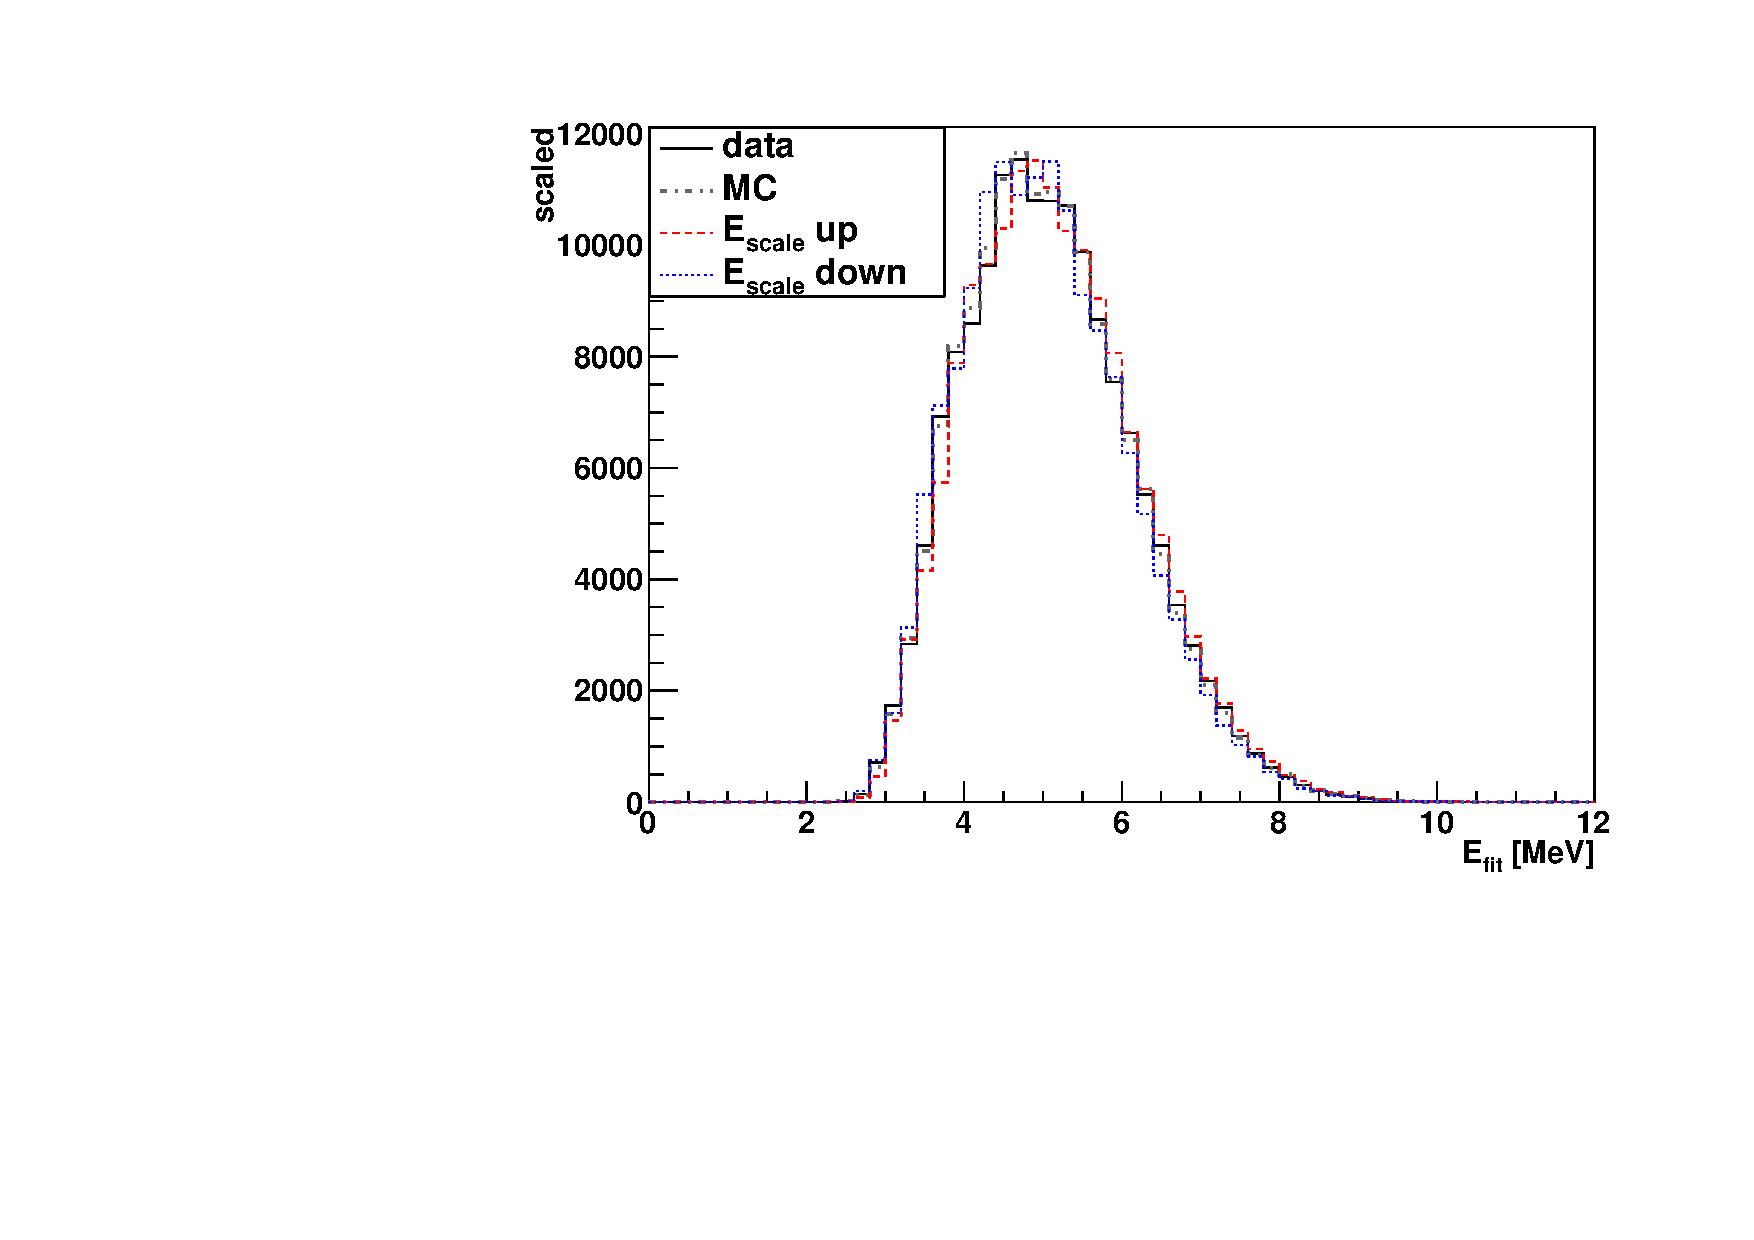
\includegraphics[width=10cm]{SmearedEscale_N16.pdf}
	\caption[Smeared reconstructed energy spectrum of $^{16}$N central run 107055.]{Smeared reconstructed energy spectrum of $^{16}$N central run 107055. The solid black line is for data and the gray dash-dot line is for unsmeared MC; the red dash line is for scaling up the $E_{fit}$ in MC; the blue dot line is for scaling down the $E_{fit}$ in MC. Histograms are normalized to the total counts of the data.\label{fig:EscaleSmear}}
\end{figure}

To apply the energy resolution systematics, the spectrum of the reconstructed energy $E_{fit}$ is convolved with an additional Gaussian resolution function $\mathrm{Gaus}(0,\sigma_\mathrm{smear})$, where $\sigma_\mathrm{smear}=\sqrt{E_{fit}} \; \sqrt{(1+\Delta_{b})^2-1}$. To smear the $E_{fit}$ event by event, $E_\mathrm{smear}$ is randomly sampled from $\mathrm{Gaus}(0,\sigma_\mathrm{smear})$, and then $E'_{fit}=E_{fit}+E_\mathrm{smear}$. Fig.~\ref{fig:EresolSmear} shows the effects of smearing the energy resolution on the $E_{fit}$ spectrum of the $^{16}$N central run 107055. It is obvious that smearing with the additional resolution coming from the uncertainties in $b$ widens the $E_{fit}$ spectrum. Because there is no unfolding procedure to improve or narrow the energy resolution, this energy resolution systematic is one-sided\cite{marzec2019measurement}. Therefore, in the analysis in Chapter 6, I simply took symmetric uncertainties with different signs.
\begin{figure}
	\centering
	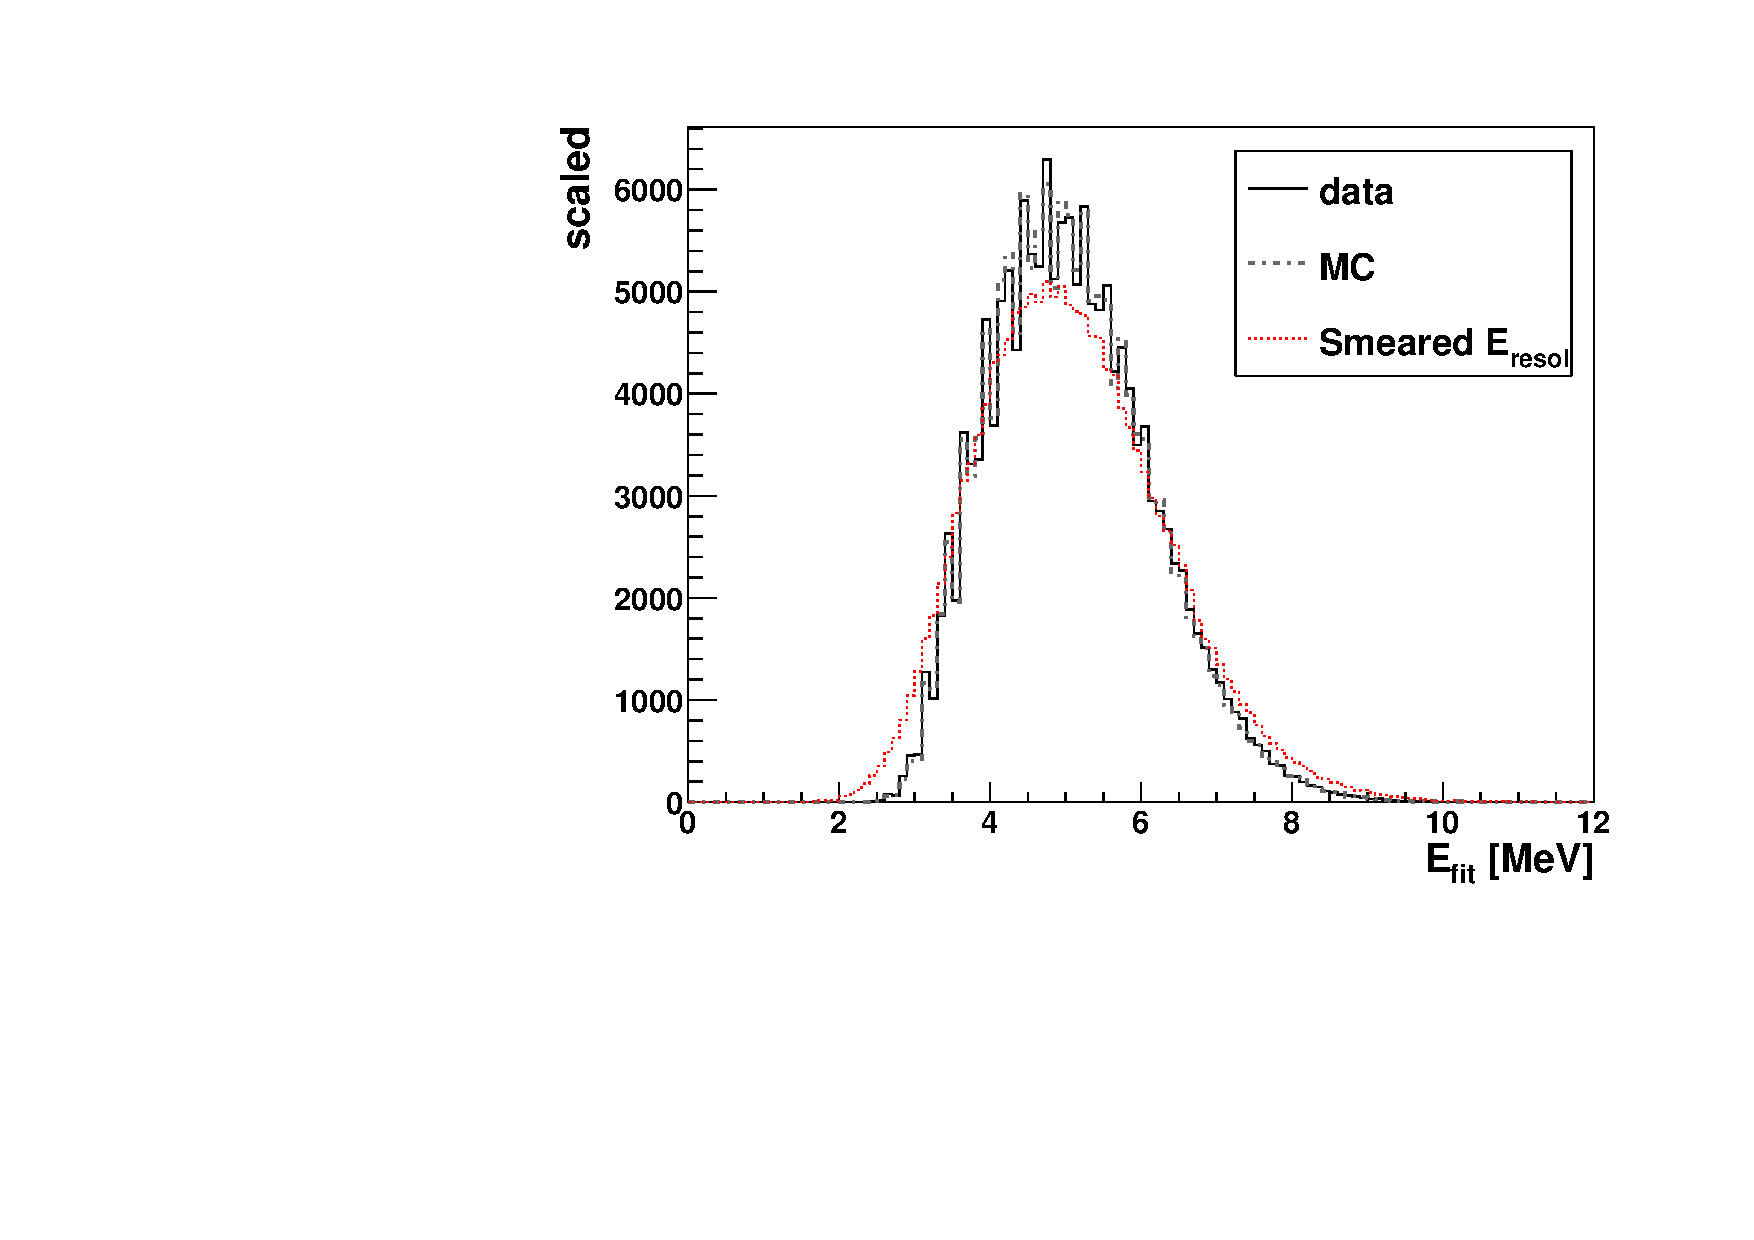
\includegraphics[width=10cm]{SmearedEresol_N16_new.pdf}
	\caption[Smeared reconstructed energy spectrum of $^{16}$N central run 107055.]{Smeared reconstructed energy spectrum of $^{16}$N central run 107055. The red dash line is for smearing the $E_{fit}$ with $\mathrm{Gaus}(E_{fit},\sigma)$. Histograms are normalized to the total counts of the data.\label{fig:EresolSmear}}
\end{figure}
